\documentclass[]{book}
\usepackage{lmodern}
\usepackage{amssymb,amsmath}
\usepackage{ifxetex,ifluatex}
\usepackage{fixltx2e} % provides \textsubscript
\ifnum 0\ifxetex 1\fi\ifluatex 1\fi=0 % if pdftex
  \usepackage[T1]{fontenc}
  \usepackage[utf8]{inputenc}
\else % if luatex or xelatex
  \ifxetex
    \usepackage{mathspec}
  \else
    \usepackage{fontspec}
  \fi
  \defaultfontfeatures{Ligatures=TeX,Scale=MatchLowercase}
\fi
% use upquote if available, for straight quotes in verbatim environments
\IfFileExists{upquote.sty}{\usepackage{upquote}}{}
% use microtype if available
\IfFileExists{microtype.sty}{%
\usepackage{microtype}
\UseMicrotypeSet[protrusion]{basicmath} % disable protrusion for tt fonts
}{}
\usepackage[margin=1in]{geometry}
\usepackage{hyperref}
\hypersetup{unicode=true,
            pdftitle={JABSTB: Statistical Design and Analysis of Experiments with R},
            pdfauthor={TJ Murphy PhD, Department of Pharmacology, School of Medicine, Emory University, Atlanta, GA biostats538@gmail.com},
            pdfborder={0 0 0},
            breaklinks=true}
\urlstyle{same}  % don't use monospace font for urls
\usepackage{natbib}
\bibliographystyle{apalike}
\usepackage{color}
\usepackage{fancyvrb}
\newcommand{\VerbBar}{|}
\newcommand{\VERB}{\Verb[commandchars=\\\{\}]}
\DefineVerbatimEnvironment{Highlighting}{Verbatim}{commandchars=\\\{\}}
% Add ',fontsize=\small' for more characters per line
\usepackage{framed}
\definecolor{shadecolor}{RGB}{248,248,248}
\newenvironment{Shaded}{\begin{snugshade}}{\end{snugshade}}
\newcommand{\AlertTok}[1]{\textcolor[rgb]{0.94,0.16,0.16}{#1}}
\newcommand{\AnnotationTok}[1]{\textcolor[rgb]{0.56,0.35,0.01}{\textbf{\textit{#1}}}}
\newcommand{\AttributeTok}[1]{\textcolor[rgb]{0.77,0.63,0.00}{#1}}
\newcommand{\BaseNTok}[1]{\textcolor[rgb]{0.00,0.00,0.81}{#1}}
\newcommand{\BuiltInTok}[1]{#1}
\newcommand{\CharTok}[1]{\textcolor[rgb]{0.31,0.60,0.02}{#1}}
\newcommand{\CommentTok}[1]{\textcolor[rgb]{0.56,0.35,0.01}{\textit{#1}}}
\newcommand{\CommentVarTok}[1]{\textcolor[rgb]{0.56,0.35,0.01}{\textbf{\textit{#1}}}}
\newcommand{\ConstantTok}[1]{\textcolor[rgb]{0.00,0.00,0.00}{#1}}
\newcommand{\ControlFlowTok}[1]{\textcolor[rgb]{0.13,0.29,0.53}{\textbf{#1}}}
\newcommand{\DataTypeTok}[1]{\textcolor[rgb]{0.13,0.29,0.53}{#1}}
\newcommand{\DecValTok}[1]{\textcolor[rgb]{0.00,0.00,0.81}{#1}}
\newcommand{\DocumentationTok}[1]{\textcolor[rgb]{0.56,0.35,0.01}{\textbf{\textit{#1}}}}
\newcommand{\ErrorTok}[1]{\textcolor[rgb]{0.64,0.00,0.00}{\textbf{#1}}}
\newcommand{\ExtensionTok}[1]{#1}
\newcommand{\FloatTok}[1]{\textcolor[rgb]{0.00,0.00,0.81}{#1}}
\newcommand{\FunctionTok}[1]{\textcolor[rgb]{0.00,0.00,0.00}{#1}}
\newcommand{\ImportTok}[1]{#1}
\newcommand{\InformationTok}[1]{\textcolor[rgb]{0.56,0.35,0.01}{\textbf{\textit{#1}}}}
\newcommand{\KeywordTok}[1]{\textcolor[rgb]{0.13,0.29,0.53}{\textbf{#1}}}
\newcommand{\NormalTok}[1]{#1}
\newcommand{\OperatorTok}[1]{\textcolor[rgb]{0.81,0.36,0.00}{\textbf{#1}}}
\newcommand{\OtherTok}[1]{\textcolor[rgb]{0.56,0.35,0.01}{#1}}
\newcommand{\PreprocessorTok}[1]{\textcolor[rgb]{0.56,0.35,0.01}{\textit{#1}}}
\newcommand{\RegionMarkerTok}[1]{#1}
\newcommand{\SpecialCharTok}[1]{\textcolor[rgb]{0.00,0.00,0.00}{#1}}
\newcommand{\SpecialStringTok}[1]{\textcolor[rgb]{0.31,0.60,0.02}{#1}}
\newcommand{\StringTok}[1]{\textcolor[rgb]{0.31,0.60,0.02}{#1}}
\newcommand{\VariableTok}[1]{\textcolor[rgb]{0.00,0.00,0.00}{#1}}
\newcommand{\VerbatimStringTok}[1]{\textcolor[rgb]{0.31,0.60,0.02}{#1}}
\newcommand{\WarningTok}[1]{\textcolor[rgb]{0.56,0.35,0.01}{\textbf{\textit{#1}}}}
\usepackage{longtable,booktabs}
\usepackage{graphicx,grffile}
\makeatletter
\def\maxwidth{\ifdim\Gin@nat@width>\linewidth\linewidth\else\Gin@nat@width\fi}
\def\maxheight{\ifdim\Gin@nat@height>\textheight\textheight\else\Gin@nat@height\fi}
\makeatother
% Scale images if necessary, so that they will not overflow the page
% margins by default, and it is still possible to overwrite the defaults
% using explicit options in \includegraphics[width, height, ...]{}
\setkeys{Gin}{width=\maxwidth,height=\maxheight,keepaspectratio}
\IfFileExists{parskip.sty}{%
\usepackage{parskip}
}{% else
\setlength{\parindent}{0pt}
\setlength{\parskip}{6pt plus 2pt minus 1pt}
}
\setlength{\emergencystretch}{3em}  % prevent overfull lines
\providecommand{\tightlist}{%
  \setlength{\itemsep}{0pt}\setlength{\parskip}{0pt}}
\setcounter{secnumdepth}{5}
% Redefines (sub)paragraphs to behave more like sections
\ifx\paragraph\undefined\else
\let\oldparagraph\paragraph
\renewcommand{\paragraph}[1]{\oldparagraph{#1}\mbox{}}
\fi
\ifx\subparagraph\undefined\else
\let\oldsubparagraph\subparagraph
\renewcommand{\subparagraph}[1]{\oldsubparagraph{#1}\mbox{}}
\fi

%%% Use protect on footnotes to avoid problems with footnotes in titles
\let\rmarkdownfootnote\footnote%
\def\footnote{\protect\rmarkdownfootnote}

%%% Change title format to be more compact
\usepackage{titling}

% Create subtitle command for use in maketitle
\newcommand{\subtitle}[1]{
  \posttitle{
    \begin{center}\large#1\end{center}
    }
}

\setlength{\droptitle}{-2em}

  \title{JABSTB: Statistical Design and Analysis of Experiments with R}
    \pretitle{\vspace{\droptitle}\centering\huge}
  \posttitle{\par}
    \author{TJ Murphy PhD, Department of Pharmacology, School of Medicine, Emory University, Atlanta, GA \href{mailto:biostats538@gmail.com}{\nolinkurl{biostats538@gmail.com}}}
    \preauthor{\centering\large\emph}
  \postauthor{\par}
      \predate{\centering\large\emph}
  \postdate{\par}
    \date{2018-12-30}

\usepackage{booktabs}

\begin{document}
\maketitle

{
\setcounter{tocdepth}{1}
\tableofcontents
}
\hypertarget{preface}{%
\chapter*{Preface}\label{preface}}
\addcontentsline{toc}{chapter}{Preface}

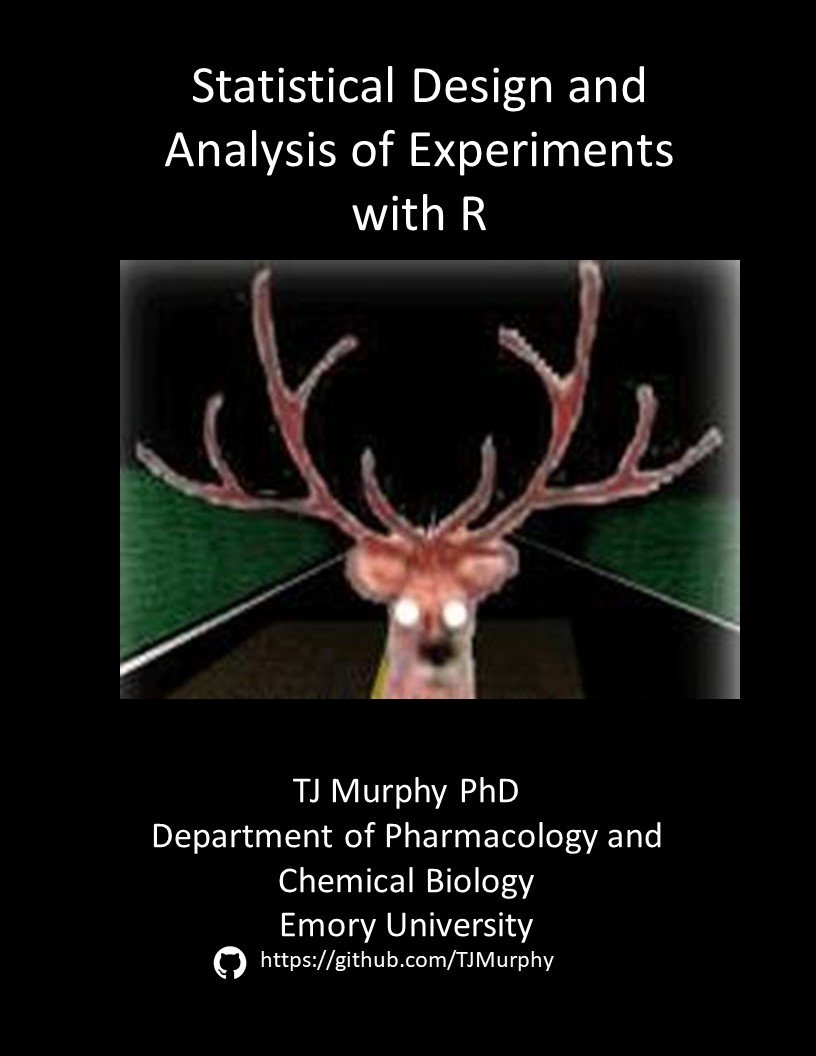
\includegraphics[width=11.33in]{images/book_cover}

This book is a resource for students enrolled in my biostats course.

The students are primarily in one of Emory's biomedical and biological sciences PhD programs. There are the ocassional Emory honors program undergrads, students from Emory's public health school, and usually a few Georgia Tech graduate students, also.

When you teach stats you have to choose software and maybe a textbook. I'd been wrestling with the decision to switch my course over to R for a few years, but never really found the right stats book that covers the subject the way I like to emphasize.

When I finally took the plunge I needed to prepare a bunch of handouts with coding examples for the various types of analyses I'd been teaching. Then I decided to write some intro handouts.

Before you know it, you have a ``book''. This is that. JABSTB.

Not included in this book are additional materials for the course (eg, take home and group exercises, slide decks, data sets, my extensive collection of stats cartoons, etc).

The scope of the book is to provide a) some background on statistical fundamentals that are most relevant to the biomedical researcher who is testing ideas by generating data (sampling, error, statistical hypotheses, experimental design) and then, b) provide examples for running and interpreting various statistical functions.

These are meant to be starting points. What's really nice about R is its adaptability. Copy and paste my examples into your R script or R markdown file, understand how they work by trying to break them, and then get to work modifying them for your own purposes.

Most chapters have code that require R packages beyond those that come in the base R installation. Those are listed at the head of each chapter.

Each chapter has a corresponding RMarkdown document. If you wish to grab those documents instead of using this material as HTML, go grab it on Github. Simply fork, clone or download them from the \href{https://github.com/TJMurphy/jabstb}{Github jabstb repo}. You'll just need the Rmd files.

All of the other files are there for publishing this up as bookdown. By the way, I've optimized these Rmd's to make good HTML pages. I have not even checked to see if they work as PDFs.

This book is a living document. It is subject to a lot of on-the-fly revision. Stuff will be added and eliminated over time.

As I write these words, in Dec 2018, my main disclaimer is that it is definitely an MVP.

If you find errors, have any suggestions, or would otherwise like to contribute, I welcome your help. Please submit a pull request and/or contact me by email. I welcome your additions.

Copyright 2018 © TJ Murphy MIT license.

\hypertarget{author}{%
\chapter{About the author}\label{author}}

A few years ago I adopted this course from Frank Gordon, a colleague who had retired. Like Frank, I'm a biomedical scientist who happens to have high level of interest in statistical methods.

I learned this material as a graduate student at Mizzou. There I took several stats courses as electives. The ones that impacted me the most were taught by the late Gary Krause, then a professor and statistician in Mizzou's agricultural college.

The light turned on for me during Gary's \emph{Experimenal Design} course. That's when the fog of mathematical statistics cleared enough so I could finally ``get'' the pragmatic value of statistics for the researcher.

What became most clear is that experimental design is a statistical framework for conducting unbiased research. That concept permeates my course and this book.

I was working on my PhD in pharmacology within the medical school. But most of my classmates in Gary's courses were working on a PhD in one of the agriculture programs, usually in some area of agronomy or in animal science.

The problem my classmates shared, which was not one that really affected me, is having one growing or mating season by which to run a fully replicated experiment.

One shot.


\includegraphics[width=12.21in]{images/my_shot}

That one shot changes everything.

Planning was a priority for them. They needed to map out their experimental design in advance. Once the experiment began, any new wrinkles or oversights would have to wait until the next growing season. They didn't have the luxury of running out to the field to plant another row of the crop, or to arrange additional breeding groups.

Planning was based upon statistical design principles, often in consultation with Gary. Statistics were \emph{a priori} planning and \emph{post-hoc} tests. At the end of the season the samples were harvested. After all the biochemistry was completed at their lab benches, the final statistical analysis was performed according to the planned approach.

In contrast, it is fair to say that most biomedical scientists fail to incorporate statistical design into their plans. That failure opens up a whole can of worms that can generally be characterized as doing statistics in ways it was never meant to be done.

All too common is the biomedical researchers who takes a more ``fly by the seat of their pants'' approach to running experiments and collecting data. In this approach, bunches of near and partial replicates are munged together before looking at the results and making a decision about what statistical analysis would be most appropriate to confirm their inclined interpretation.

Unfortunately, that approach is riddled with biases, and sometimes other negative consequences that are even more challenging.

Experimental statistics was invented by the founders as a means of instilling some structure into the planning, discovery and inference process so that unbiased interpretations can be made.

The focus of this course is in teaching statistics as experimental design. The ideal learner will finish the course knowing how to map out the statistical plan for an experiment in advance and appreciate why this is so important to reduce bias.

That same learner will also know how to analyze, interpret, visualize, and write up the results for a wide array of experimental designs. Most of which she will forget immediately.

And since I emphasize pre-planning, this book is full of simulations. That's the really great advantage of using R to teach biostats, in my view.

I'm not a mathematician so I only offer enough theoretical and mathematical statistics to provide a glimpse of how how things work ``under the hood''. When I do, it is mostly for stuff I think is helpful to interpret statistical output, or illustrate why a test works in a specific way. I very much believe there is an important place for mathematical statistics, I just don't believe I'm the person who should be teaching it.

Scientists have a lot of overt biases and are the last to realize it. Data frequently has a lot of hidden biases we fail to see. That's why operating within a statistical design framework is so important.

For the biomedical PhD student hoping to graduate while still young, a statistical design framework also offers potential to keep things rolling downhill for you. Statistical thinking should help you avoid the time-sucking rabbit holes that are associated with sloppy, inconclusive or uninterpretable experiments and prolonged time to degrees.

\hypertarget{history}{%
\chapter{A Brief History of Experimental Design}\label{history}}

Researchers in the pre-statistics days lacked the statistical framework that today's researchers take for granted. Our ancestor scientists were remarkably adept at the scientific method, in making observations, and in collecting data with great care. However, they struggled with designing experiments, in summarizing the data, and in drawing unbiased inference from it.

The statistical approach to experimental design we use today was first enumerated about a century ago, largely by Sir RA Fisher. His story is interesting in part because it is just so classically accidental.

\begin{figure}
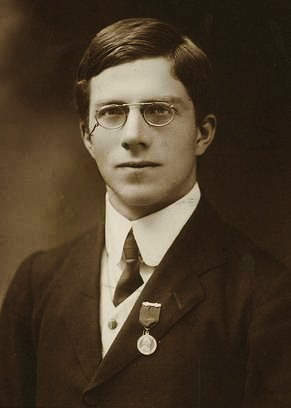
\includegraphics[width=4.04in]{images/ra_fisher} \caption{RA Fisher in 1913, from the [Adelaide Digital Archive](https://digital.library.adelaide.edu.au/dspace/handle/2440/3860)}\label{fig:unnamed-chunk-4}
\end{figure}

At the outset of his career Fisher did not foresee authoring the foundational principles of experimental design and statistics practiced by most of us today. He took that trajectory by accident.

For about five years after graduating from Cambridge, Fisher worked as a census bureaucrat and part time math teacher.

He was smitten by Darwin's theory of evolution, which was the hot discovery of the day, of course. Fisher's side hustle was to work on mathematical problems related to evolutionary genetics. Today, we would probably recognize him as a hobbyist quantitative geneticist or perhaps even as one of the first bioinformaticians. That's certainly where his career ambitions seem laid. He never lost an interest in evolution and would go on to become, unfortunately, a prominent eugenicist. The take-away from that, alone, is that statistics is not a fool-proof antibias framework.

Still, one big contribution he made during this early stage was no small feat. He defined variance as the square of the standard deviation. He proposed that variance is useful as a descriptive statistic for the variability within a population. Further developed, it would soon become the foundation of the multigroup exprimental designs that called ANOVA, the analysis of variance, which are widely used today.

In 1919 Fisher was hired as a temporary statistician by Sir John Russell, the new director of the Rothamsted Experimental Research center in England.

After decades of underfunding Rothamsted had become a bit rundown. Russell, an agricultural chemist who today we would probably categorize as a biochemist, was hired to beef up postwar (WWI) agricultural research in the UK. Upon arrival he realized the station had a large repository of data. Fully expecting to create even more under his leadership. Russell believed bringing a mathematician on board could help him make sense of this data repository.

Thus, Russell hired Fisher to take a temporary position. Today, we would recognize Fisher in his Rothamsted role as a freelance data scientist charged with conjuring meaning from reams of the station's data, some of which represented serial experiments that had been running for decades.

As he dug in Fisher saw a lot of flaws in the Rothamsted dataset. He had difficulty making sense of much of it. Mostly because the experiments were, in his view, so poorly designed the results were uninterpretable. If that sounds familiar then I've achieved my objective for mentioning it.

Here's when the paradigm shifted. Fisher began to think about the process by which experimental data \textbf{should} be collected. Almost immediately after digging into his Rothamsted work he invented concepts like confounding, randomization, replication, blocking, the latin square and other factorial designs. As I mentioned above, his invention of the \textbf{analysis of variance} extended his prior work on variance. The procedure of maximum likelihood estimation soon followed, as well.

It was a truly remarkable period. In 1925 Fisher published a small book, \href{https://psychclassics.yorku.ca/Fisher/Methods/}{\emph{Statistical Methods for Research Workers}}. In 1934 he published its extension, \href{https://www.phil.vt.edu/dmayo/PhilStatistics/b\%20Fisher\%20design\%20of\%20experiments.pdf}{\emph{Design of Experiments}}. In these works lay the foundations of how researchers today approach their experiments. His statistical procedures, developed with agricultural science in mind, would soon cross oceans\ldots{}and then disciplines.

Today, experiments that we would recognize as statistically rigorous are those in which Fisher's early principles operate as procedures. We know today that randomization and pre-planned levels of replication are essential for doing unbiased research. The block ANOVA designs he mapped out then are among the most common experimental designs that we see in the biological and biomedical literature today.

There's much more to this history, including many additional players and plenty of controversy that remains unsettled to this day. I emphasize Fisher mostly because his experimental design and analysis procedures remain the standard for prospective experiments today.

\hypertarget{bigpic}{%
\chapter{The Big Picture}\label{bigpic}}

\emph{To call in the statistician after the experiment is done may be no more than asking him to perform a post-mortem examination: he may be able to say what the experiment died of. \textasciitilde{} Sir Ronald Aylmer Fisher}

\begin{Shaded}
\begin{Highlighting}[]
\KeywordTok{library}\NormalTok{(tidyverse)}
\KeywordTok{library}\NormalTok{(Hmisc)}
\end{Highlighting}
\end{Shaded}

Let's start by listing out some key characteristics that most biomedical experiments share in common.

They\ldots{}

\begin{itemize}
\tightlist
\item
  tend to involve the use of relatively small sample sizes.
\item
  are usually highly exploratory in nature.
\item
  generate data that are either discrete counts or measurements of continuous scalars.
\item
  are structured by a small group of fairly common experimental designs.
\item
  are usually interpreted in a binary way; as having ``worked'', or not.
\item
  test hypotheses (though too often these are unstated).
\item
  aspire for rigor, replicability and reproducibility.
\item
  aspire to be unbiased.
\end{itemize}

The stakes of our work can be pretty high. These include the higher ideals such as the validation of novel scientific paradigms, the steady advancement of knowledge, and opening the door to create impactful solutions, particularly in the realm of human diseases and suffering.

But no less motivating are the issues more related to the professional practice of science. These include ego, the completely natural impulse to seek out validation for an idea, publication and/or commercialization, time to degree, career viability, scientific reputations, and coveted research/investment funds.

The point is that the process of scientific discovery is driven both by ideals and by biases. This is nothing new.

The one big concept that I hope you embrace is that the statistical design and analysis of experiments serves as a working framework within which the biomedical researcher can conduct reasonably unbiased work. The statistical approaches covered in this course, it turns out, were invented long ago with all of these drivers in mind.

\hypertarget{what-are-experimental-statistics}{%
\section{What are experimental statistics?}\label{what-are-experimental-statistics}}

Experimental statistics are used

\begin{itemize}
\tightlist
\item
  to summarize data into simpler descriptive models.
\item
  as procedures to draw inferences from samples.
\item
  as procedures that guide the design of experiments.
\item
  to serve as framework for conducting unbiased research.
\end{itemize}

Chances are you thought biostats was just one or two of those bullets, and probably not the latter two.

\hypertarget{descriptive-modeling}{%
\subsection{Descriptive modeling}\label{descriptive-modeling}}

Statistical models are ways of simplifying or summarizing data so that they can be more readily described and interpreted.

For example, if we have a sample in which blood glucose levels are measured in each of many subjects, clarity demands we explain those results in terms of summary statistics. Thus, we use parameters like the sample mean and standard deviation, or median and ranges or percentiles. The alternative is unthinkable today (but common long ago), which is to discuss each replicate individually.

To emphasize that sample parameters differ from population parameters, the standard in statistical notation is to use roman characters to indicate samples and greek characters to indicate the population. For example,

\begin{longtable}[]{@{}rrr@{}}
\toprule
parameter & sample & population\tabularnewline
\midrule
\endhead
mean & \(\bar y\) & \(\mu\)\tabularnewline
standard deviation & \(s\) & \(\sigma\)\tabularnewline
variance & \(s^2\) & \(\sigma^2\)\tabularnewline
\bottomrule
\end{longtable}

Thus, the sample mean, \(\bar y\) is an estimate of the population mean, \(\mu\).

Statistical tests also have a descriptive element in that they convey information about the experimental design. If you say, ``I'm working up a two-tailed paired t-test,'' say no more. From that alone I know something about your hypothesis, how your replicates are handled, the number of predictor groups, and the type of data you're measuring.

Regression models also describe data. For example, here is the well-known Michaelis-Menten model that describes product formation as a function of substrate concentration.\\
\[[P]=\frac{[S][Vmax]}{[S]+Km}\]

That's a model we might fit to certain kinds of enzyme kinetic data, because we use it to estimate scientifically meaningful parameters, like \(V_{max}\) and \(K_m\).

In fact, mathematical statistics is actually just modeling. Modeling is the process of simplifying data into something more coherent.

Take a simple example of two groups shown here. Each group has been fit to a simple model: that for the mean and standard deviation. Clearly, that model fits the control group much better than it fits the treatment group.

\begin{figure}

{\centering 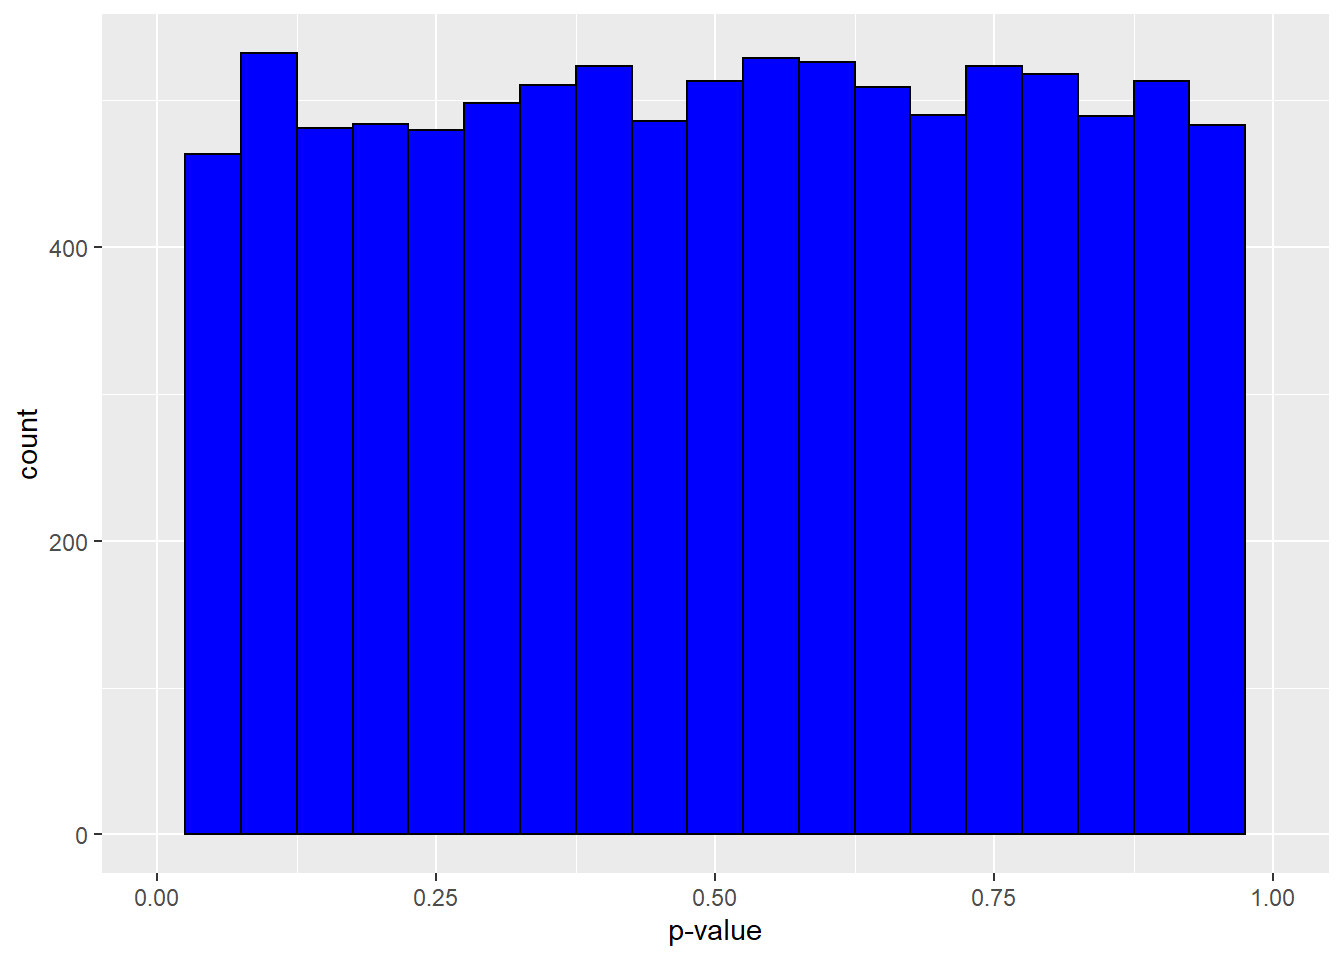
\includegraphics{jabstb_files/figure-latex/unnamed-chunk-6-1} 

}

\caption{Is the mean for each these groups a good descriptive model?}\label{fig:unnamed-chunk-6}
\end{figure}

Why do I say that? The treatment group data are much more skewed. Most of the data values are greater than the mean of the group. Sure, a mean can be calculated for that group, but it serves as a fairly crappy summary. Perhaps some other model (or group of statistical parameters) would better convey how these data behave?

This is to point out that learning statistics is about learning to make judgments about which models are best for describing a given data set.

\hypertarget{statistical-inference}{%
\subsection{Statistical inference}\label{statistical-inference}}

There are two main types of inference researchers make.

One type is to infer whether an experiment ``worked'' or not\ldots{}the so-called ``significance test''. This familiar process involves calculating a test statistic from the data (eg, t-test, F-tests, etc) and then applying a threshold rule to its value. If the test passes the rule, we conclude the experiment worked. I cover this type of inference in much more detail in the p-value chapter \ref{pvalues}, and we'll talk about it over and again throughout the course.

A second type of inference is to extrapolate from a sample some \textbf{estimate} for the values of the variables within the population that was sampled.

Both descriptive and statistical inference are subject to error. By random chance alone our sample could be way off the mark, even with perfectly calibrated instrumentation.

The real difficulty with inference is we can never know for certain whether we are right or wrong.

They are called random variables for a reason. It pays to have a very healthy respect for the role played by random chance in determining the values of our parameter estimates. If we were to completely redo a fully replicated experiment once more, we would almost certainly arrive at different numbers. In a well behaved system, they'd likely be in the same ballpark as those of the first experiment. But they would still differ.

To illustrate, copy and paste the code chunk below. It replicates a random triplicate sample six times, taking six means. Unlike in real life, the population parameters are known (because I coded them in): \(\mu=2\) and \(\sigma=0.4\). You can run that chunk tens of thousands of times and never get a ``sample'' with one mean that has a value of exactly 2, even though that's the true mean of the population that was sampled.

\begin{Shaded}
\begin{Highlighting}[]
\NormalTok{x <-}\StringTok{ }\KeywordTok{replicate}\NormalTok{(}\DecValTok{6}\NormalTok{, }\KeywordTok{rnorm}\NormalTok{(}\DecValTok{3}\NormalTok{, }\DecValTok{2}\NormalTok{, }\FloatTok{0.4}\NormalTok{))}
\KeywordTok{apply}\NormalTok{(x, }\DecValTok{2}\NormalTok{, mean)}
\end{Highlighting}
\end{Shaded}

\begin{verbatim}
## [1] 2.055037 1.770020 2.174044 1.855520 1.997851 2.437189
\end{verbatim}

\hypertarget{experimental-design}{%
\subsection{Experimental design}\label{experimental-design}}

Experimental planning that involves dealing with statistical issues is referred here as experimental design.

This involves stating a testable statistical hypothesis and establishing a series of decision rules in advance of data collection. These rules range from subject selection and arrangement, predetermination of sample size using \emph{a priori} power analysis, setting some data exclusion criteria, defining error tolerance, specifying how the data will be transformed and analyzed, declaring a primary outcome, on up to what statistical analysis will be performed on the data.

Experimental design is very common in \href{https://clinicaltrials.gov/ct2/home}{prospective clinical research}. Unfortunately, very few basic biomedical scientists practice anything remotely like this. Most biomedical researchers begin experiments with only vague ideas about the statistical analysis, which is usually settled on after the fact. Much of the published work today is therefore retrospective, rather than prospective. Yet, most researchers tend to use statistics that are largely intended for prospective designs. That's a problem.

\hypertarget{statistics-as-an-anti-bias-framework}{%
\subsection{Statistics as an anti-bias framework}\label{statistics-as-an-anti-bias-framework}}

If you are ever asked (for example, in an examination) what purpose is served by a given statistical procedure, and you're not exactly sure, you would be wise to simply offer that it exists to prevent bias. That may not be the answer the grader was hunting for, but it is almost surely correct.

The main purpose of ``doing'' statistical design and analysis of experiments is to control for bias. Humans are intrinsically prone to bias and scientists are as human as anybody else. Holding or working on a PhD degree doesn't provide us a magic woo-woo cloak to protect us from our biases.

Therefore, whether we choose to admit it or not, bias infects everything we do as scientists. This happens in subtle and in not so subtle ways. We work hard on our brilliant ideas and, sometimes, desperately wishing to see them realized, we open the door to all manner of bias.

Here are some of the more important biases.

\#\#\#\#Cognitive biases

From a statistical point of view biases can be classified into two major groupings. The first are \href{https://en.wikipedia.org/wiki/List_of_cognitive_biases}{Cognitive biases}. These are how we think (or fail to think) about our experiments and our data.

These frequently cause us to make assumptions that we would not if we only knew better or were wired differently. If you ever find yourself declaring, ``how could this not work!'' you are in the throes of a pretty deep cognitive bias. In bench research, cognitive biases can prevent us from building adequate controls into experiments or lead us to draw the wrong interpretation of results, or prevent us from spotting confounding variables or recognizing telling glitches in the data as meaningful.

\#\#\#\#Systematic biases

The second are systematic biases. Systematic biases are inherent to our experimental protocols, the equipment and materials we use, the timing and order by which tasks are done, the subjects we select and, yes (metaphorically), even whether the data are collected left-handed or right-handed, and how data is handled or transformed.

Systematic biases can yield the full gamut of unintended outcomes, ranging between nuisance artifacts to false negatives or false positives. For example, poorly calibrated equipment will bias data towards taking inaccurate values. Working forever on an observed phenomenon using only one strain of mouse or cell line may blind us from realizing it might be a phenomenon that only occurs in that strain of mouse or cell line.

\#\#\#\#Scientific misconduct

More malicious biases exist, too. These include \href{https://grants.nih.gov/policy/research_integrity/index.htm}{forbidden practices such as data fabrication and falsification}. This is obviously a problem of integrity. Very few scientists working today are immune from the high stakes issues that pose threats to our sense of integrity.

In the big picture, particularly for the biomedical PhD student, I like to call bias the event horizon of rabbit holes. A rabbit hole is that place in a scientific career where it is easy to get lost for a long, long time. You want to avoid them.

The application of statistical principles to experimental design provides some structure to avoid making many of the mistakes that are associated with these biases. Following a well-considered, statistically designed protocol enforces some integrity onto the process of experimentation. Most scientists find a statistical framework quite livable.

If you give it some thought, the only thing worse than a negative result from a statistically rigorous experiment is a negative result from a statistically weak experiment. With the former at least you know you've given it your best shot. That is hard to conclude when the latter occurs.

\hypertarget{sampling}{%
\chapter{Statistical Sampling}\label{sampling}}

\emph{An experiment is no more reliable than is its sample. -TJ Murphy}

A statistically valid sample is comprised of independent replicates of the experimental unit, which are generated using some random process.

To unpack this let's think about each of the following terms:

\begin{itemize}
\tightlist
\item
  What are experimental units?
\item
  What do we mean by independent replicates?
\item
  What is a random process?
\item
  When is statistical validity even important?
\end{itemize}

\hypertarget{experimental-units}{%
\section{Experimental units}\label{experimental-units}}

\textbf{The experimental unit is the source of the measurement. An experimental unit can generate one or many measurement values.}

I prefer the concept of an experimental unit to the concept of subject, though they often mean the same thing. I've found the word subject carries more ambiguity, especially for people first learning sampling and sample size concepts.

In some experimental designs (eg, unpaired or completely randomized) each experimental unit generates a single measurement value. Here there is a one-to-one correspondence exists between the number of experimental units and the number of measurement values within a data set.

In other designs (eg, paired or matched or repeated/related measure), a single experimental unit can generate more than one measurement values for the same variable. Such data sets have more values than experimental units.

Here are some guidelines for deciding what is the experimental unit in an experiment, with full recognition that sometimes there are gray areas. Ultimately the researcher has to use scientific judgment to recognize or define the experimental unit.

\hypertarget{a-simple-test-to-define-the-experimental-unit}{%
\subsection{A simple test to define the experimental unit}\label{a-simple-test-to-define-the-experimental-unit}}

When defining an experimental unit I recommend using a simple test:

\textbf{Are these measurements intrinsically-linked?}

If two or more measurement values are intrinsically-linked then they would comprise paired or matched or related measures from a single experimental unit.

So how could you judge whether two or more measurements are intrinsically-linked? For the most part, this happens when the source of those measurements doesn't differ.

Here are a few examples:

\emph{A before and after design.} A mouse is scored on how well it performs a behavioral test at baseline, before a treatment. After that same mouse receives a treatment it is run through the behavioral test once more to get a second score. Those two scores are intrinsically-linked because they were taken from the same mouse. All that differs between the scores is the absence or presence of the treatment, the effect of which the researcher is trying to measure.

We would also say those two scores are matched, paired or related/repeated measures. A single mouse from which two scores are derived is an independent replicate of the experimental unit.

\emph{Twinning.} Take for example a study involving human identical twins. In these studies identical twin pairs are modeled as a single experimental unit due to their high level of instrinsic relatedness. There are two human subjects but they are modeled statistically as a single experimental unit. The two measurements would be analyzed using a statistical method configured for paired or matched or repeated/related measures.

One of the pair receives a control condition while the other receives a treatment condition. A measurement is taken from each person. There are two measurements in total, and two people, but only a single experimental unit. Given that the twins are so identical we could reasonably conclude these two measurements are intrinsically-linked. We can model the pair as one.

The two measurements would be analyzed using a statistical method configured for paired or matched or repeated/related measures.

\emph{Unpaired or completely randomized} In contrast, imagine a study using the same control and treatment conditions using unrelated humans (or some other outbred animal species) as subjects. Each subject is assigned either a treatment or a control, and only a single measurement is taken from them. Since the subjects are each very different from each other, we could not conclude that measurements taken from them are intrinsically-linked. Each person stands alone as an experimental unit. The data would be analyzed using an unpaired, unmatched or completely randomized test.

\textbf{Intrinsically-linked measurements are very common in bench work. In fact they are too often overlooked for what they are and mistakenly analyzed as unmatched. Experiments involving batches of biological material, cultured cells and/or littermates of inbred animal strains routinely involve intrinsically-linked measurements. As a general rule, these should always be designed and analyzed using matched/paired/related measures procedures.}

\emph{Cell cultures} Cell cultures are remarkably homogeneous. The typical continuous cell line is a monoculture passaged across many doubling generations.

Imagine a test conducted on a 6 well multi-well cell culture plate. Each well receives a different level of some treatment condition, such as a dosing or time-course study.

All of the wells were laid down at the same time from a common batch of cells. Each well is very highly related to all of the other wells. The intrinsic differences between wells would be relatively minor and mostly due to technical variation. There's no real inherent biological variation from well-to-well other than that attributable to the level of treatment the well receives.

As a result, all of the measurements taken from a plate of wells are intrinsically-linked to each other. The experimental unit is the plate. They should be designed and analyzed using matched/paired/related measure statistical procedures.

Furthermore, any other plates laid down at the same time from the same source of cells are virtually identical clones of each other. If we were to expose the wells in all of those plates to various treatments followed by taking some measurement, then it is pretty easy to argue that all of those measurements taken on that passage of cells are intrinsically-linked. None of the wells are independent of any of the other wells, irrespective of the plate. Together, all of the plates represent a single experimental unit.

\emph{Inbred mice} In many regards, the high level of relatedness within inbred mouse strains doesn't differ from human identical twins, or from cultured cells, for that matter.

A given strain of these animals are inbred to genetic homogeneity across several generations. For all intents and purposes all mice derived from a given strain are immortalized clones of each other. Two mice from the same litter are identical twins. Indeed, two mice from different litters from the same strain are identical twins.

Due to their clonal identity all measurements taken from any of these highly related subjects are intrinsically-linked.

Just as for cell culture, protocols must be contrived to break up the homogeneity. A common approach is to treat the litter as the experimental unit and take measures from littermates as intrinsically-linked.

\emph{Split tissue} Imagine two slices of an organ (or two drops of blood) taken from a single animal. Although the two slices (or drops of blood) are obviously different from each other, any measurements derived from each are intrinsically-linked. The experimental unit would be the animal from which that biological material is derived.

\emph{Batches} Finally, imagine a batch of a purified protein or other biochemical material. The batch was isolated from a single source and prepared through a single process. The material in the batch is highly homogeneous, irrespective of whether it is stored away in aliquots. Any measurement taken from that batch are highly related to any other measurement. They are intrinsically-linked. The batch would be the experimental unit.

\#\#\#Blocking

We have to contrive protocols to break up experimental units that have high inherent homogeneity. The statistical jargon used for this is blocking, such that blocks are essentially grouping factors that are not scientifically interesting.

Going back to culture plates. Let's say we prepared three plates on Friday. An assay performed on one plate on Monday would represent one experimental unit of intrinsically-linked measures. An assay repeated on Tuesday on a second plate would represent a second experimental unit. Wednesday's assay on the third plate is also its own experimental unit.

Here the blocking factor is the day of the week. Assuming we created fresh batches of reagents each day, there would be some day-to-day variation that wouldn't exist if we assayed all threee plates at once on a single day. But we're not particularly interested in that daily variation, either.

More conservatively, cell line passage number can be used as a blocking factor to delineate experimental units. Each passage number would represent an experimental unit and the overall replicated experiment would be said to be blocked on passage number.

Defining the experimental unit and any blocking factors requires scientific judgement. That can be difficult to do when dealing with highly homogenous material. What should be avoided is creating a design that limits random chance too severely. To measure on Monday all three plates that were laid down on Friday will probably yield tighter results than if they were blocked over the course of the week.

This has to be thought through carefully by the researcher in each and every case. Reasonable people can disagree what whether one approach is superior to some other. Therefore, what is important is to make defensible decisions. To do that, you need to think through this problem carefully. When in doubt, I suggest leaning towards giving random chance a fair shot at explaining the result you're observing.

For example, you can make the case that measurements from two cell culture plates that were laid down on the same day but are collected on different days are not intrinsically-linked. That's a harder case to make if they are collected on the same day.

You will almost certainly have to make the case that measurements taken from two mice on different days or if they are from different litters are not intrinsically-linked.

Before going there, we need to chat about what we mean by independent replication.

\hypertarget{independent-replicates}{%
\section{Independent Replicates}\label{independent-replicates}}

That we should strive for biological observations that are repeatable seems self evident.

An experiment is comprised of independent replicates of treatment conditions on experimental units. The total number of independent replicates comprises an experiment's sample size.

A primary goal in designing an experiment is to assess independent replicates that are not biased to the biological response of a more narrowly defined group of experimental units.

A replicate is therefore independent when a repeat is on an experimental unit that differs materially from a previous experimental unit. A material difference could involve a true biological replicate. Measurements taken from two unrelated human subjects have a material difference. In bench biological work with fairly homogenous systems (eg, cell lines and inbred animals) a material difference will usually need to be some separation among replicates in time and space in applying the experimental treatments.

\hypertarget{a-simple-test-for-independence}{%
\subsection{A simple test for independence}\label{a-simple-test-for-independence}}

\textbf{How willing am I to certify this is a truly repeatable phenomenon when replicated in this way?}

A new scientific discovery would be some kind of repeatable phenomenon.

\hypertarget{some-replication-examples}{%
\subsection{Some replication examples}\label{some-replication-examples}}

If we are performing an experiment using pairs of human twins, each pair that is studied stands as an independent replicate. Because the pair is the experimental unit, a study involving 5 pairs will have five, rather than ten, independent replicates.

If we conduct an experiment using unrelated human volunteers, or someother out bred animals, each person or animal from whom a measurement is recorded is considered an independent replicate. Their biological uniqueness defines their independence.

We wander into gray areas pretty quickly when thinking about the independence of experimental units in studies involving cultured cells, batches of biological material, and inbred mice. Working with these systems it is difficult to achieve the gold standard of true biological independence. The focus instead should be on repeatability\ldots{}.``Working with new batches of reagents and different days do I get the same response?''

Imagine a 6 well plate of cultured cells. No well differs biologically from any other. If each well received a repeat of the same treatment at the same time we shouldn't consider any measurements from that plate independent from others. Otherwise, the sample would be biased to that plate of cells measured at that particular time with a given set of reagents under those particular conditions. It is too biased to that moment. What if we screwed up the reagents and don't know it?

Rather than being independent, it is best to consider the 6 measurements drawn from the plate as technical replicates or pseudo replicates. The data from the 6 wells should be averaged or totaled somehow to improve the estimate of what happened on that plate that day.

A better approach with cultured cells is to use passage numbers to delineate independence. Thus, a 6 well plates from any one passage are independent experimental units relative to all other passages.

Obviously, given the homogeneity of cells in culture, it's unlikely there is much biological variation even by these criteria. But to achieve true biological independence would require re-establishing the cell line each time an independent replicate was needed. That's rarely feasible.

Inbred mice pose much the same problem. Scientific judgment is needed to decide when 2 mice from the same strain are independent of each other.

One mark of delineation is the litter. Each litter would be independent of other litters. Outcomes of two (or more) littermates could be considered matched or related-measures and thus one experimental unit.

\hypertarget{random-process}{%
\section{Random process}\label{random-process}}

You can probably sense intuitively how randomization can guard against a number of biases, both systematic and cognitive. Systematic artifacts become randomly distributed amongst the sample replicates, whereas you are less tempted to treated a replicate as preferred if you don't know what is its treatment level.

Mathematical statistics offers another important reason for randomization. In classical statistics the effect size of some treatment is assumed to be fixed. Our estimate of that real value is the problem. Thus, when we measure a value for some replicate, that value is comprised of a combination of these fixed effects and unexplained effects.

The variation we observe in our outcome variables, the reason it is a random variable, arises from these unexplained effects. These can be particularly prominent in biological systems. Randomization procedures assures those random effects are truly random. Otherwise we might mistake them for the fixed effects that are of more interest us! This concept will be discussed more formally in the section on general linear models.

Suffice to say for pragmatic purposes that random sampling is crucial for limiting intentional and unintentional researcher biases.

Either the experimental units should be selected at random, or the experimental units should be assigned treatments at random, and/or the outcome data should be evaluated at random (eg, blind). Sometimes, doing a combination of these would be even better.

Usually, the researcher supervises this randomization using some kind of random number generator. R's \texttt{sample()} function gets that job done for most situations.

Let's design an experiment that involves two treatments and a total of 12 independent experimental units. Thus, 6 experimental units will each receive either of the two treatments. Let's say that my experimental units each have an ID, in this case, a unique letter from the alphabet. Using \texttt{sample(1:12)} we randomly assign a numeric value to each ID. This numeric value will be the order by which the experimental unit, relative to the other experimental units, is subjected to the experimental treatment. ID's that are assigned even random numbers get one of the two treatments, and odd numbered ID's get the other treatment.

What we've done here is randomize both the order of replication and the assignment of treatment. That's a well-shuffled deck. You can see how this approach can be readily adapted to different numbers of treatment levels and sample sizes.

\begin{Shaded}
\begin{Highlighting}[]
\KeywordTok{set.seed}\NormalTok{(}\DecValTok{1234}\NormalTok{)}
\NormalTok{ID <-}\StringTok{ }\NormalTok{letters[}\DecValTok{1}\OperatorTok{:}\DecValTok{12}\NormalTok{]}
\NormalTok{order <-}\StringTok{ }\KeywordTok{sample}\NormalTok{(}\DecValTok{1}\OperatorTok{:}\DecValTok{12}\NormalTok{, }\DataTypeTok{replace=}\NormalTok{F)}
\NormalTok{plan <-}\StringTok{ }\KeywordTok{data.frame}\NormalTok{(ID, order)}
\NormalTok{plan}
\end{Highlighting}
\end{Shaded}

\begin{verbatim}
##    ID order
## 1   a     2
## 2   b     7
## 3   c    11
## 4   d     6
## 5   e    10
## 6   f     5
## 7   g     1
## 8   h    12
## 9   i     3
## 10  j     8
## 11  k     4
## 12  l     9
\end{verbatim}

\hypertarget{statistically-valid-samples}{%
\section{Statistically valid samples}\label{statistically-valid-samples}}

For any statistical test to be valid, each replicate within a sample must satisfy the following two criteria:

\begin{itemize}
\tightlist
\item
  The replicate should be generated by some random process.
\item
  The replicate must be independent of all other replicates.
\end{itemize}

Why? Statistical tests are one of the last stages of a hypothesis testing process. All of these tests operate, formally, on the premise that at least these two conditions are true.

When these conditions have not been met the researcher is collecting data without testing a hypothesis. To run a statsitical test is to pretend a hypothesis has been tested, when it has not.

\hypertarget{select-random-subjects}{%
\subsection{Select random subjects}\label{select-random-subjects}}

Let's say we want to do an experiment on graduate students and need to generate a representative sample. There are 5 million people in the US who are in graduate school at an given time. Let's imagine they each have a unique ID number, ranging from 1 to 5,000,000. We can use R's \texttt{sample()} function to randomly select three individuals with numbers corresponding to that range.

Sampling with replacement involves throwing a selection back into a population, where it can potentially be selected again. In that way, the probability of any selection stays the same throughout the random sampling process.

Here, the \texttt{replace\ =\ FALSE} argument is there to ensure I don't select the same individual twice.

\begin{Shaded}
\begin{Highlighting}[]
\KeywordTok{sample}\NormalTok{(}\DataTypeTok{x=}\DecValTok{1}\OperatorTok{:}\DecValTok{5000000}\NormalTok{, }\DataTypeTok{size=}\DecValTok{3}\NormalTok{, }\DataTypeTok{replace =} \OtherTok{FALSE}\NormalTok{)}
\end{Highlighting}
\end{Shaded}

\begin{verbatim}
## [1] 1413668 4617167 1461579
\end{verbatim}

All that needs to be done is to notify the three people corresponding to those IDs and schedule a convenient time for them to visit so we can do our experiment.

You can imagine several variations to randomly select graduate students for measurements. You just need a way to find graduate students, then devise a way(s) to ensure the sampling is as representative as possible. Selecting subjects from a real population is pretty straight forward, a bit like picking 8 lotto balls from a spinning container.

A lot of times in experimental work the number of subjects available to the researcher is fixed and smaller. The size of the population to be sampled can be much closer to the number of replicates needed for the experiment rather than a sample from a large pool.

In these cases we have to come up with other ways to randomize.

\hypertarget{randomize-to-sequence}{%
\subsection{Randomize to sequence}\label{randomize-to-sequence}}

For example, let's say we want to compare condition A to condition B. We have 6 subjects to work with, each of which will serve as an independent replicate. We want a balanced design so will have 3 replicates for each of the 2 conditions.

Let's imagine we can only perform an experiment on one subject, one day at a time. In that case, it makes sense to randomize treatment to sequence.

We can randomly generate a sequence of 6 even and odd numbers, and assign them to the daily sequence (MTWTFM) based on which random number is first on its list. We can make a rule that subjects assigned even numbers will receive condition A, whereas condition B is meted out to subjects associated with odd numbers.

\begin{Shaded}
\begin{Highlighting}[]
\KeywordTok{sample}\NormalTok{(}\DataTypeTok{x=}\DecValTok{11}\OperatorTok{:}\DecValTok{16}\NormalTok{, }\DataTypeTok{size=}\DecValTok{6}\NormalTok{, }\DataTypeTok{replace =} \OtherTok{FALSE}\NormalTok{)}
\end{Highlighting}
\end{Shaded}

\begin{verbatim}
## [1] 16 12 15 11 13 14
\end{verbatim}

\hypertarget{randomize-to-location}{%
\subsection{Randomize to location}\label{randomize-to-location}}

Let's imagine 3 treatments (negative control, positive control, experimental), that we will code 1,1,2,2,3,3. These will be applied in duplicate to cells on 6-well cell culture plate. We'll code the plate wells with letters, a, b, c, d, e, f from top left to bottom right (ie, a and b are wells in the top row).

Now we'll generate a random sequence of those six letters.

\begin{Shaded}
\begin{Highlighting}[]
\KeywordTok{sample}\NormalTok{(letters[}\DecValTok{1}\OperatorTok{:}\DecValTok{6}\NormalTok{], }\DataTypeTok{replace=}\NormalTok{F)}
\end{Highlighting}
\end{Shaded}

\begin{verbatim}
## [1] "b" "a" "e" "d" "f" "c"
\end{verbatim}

Next, we'll map the sequence 1,1,2,2,3,3 to those letters. Thus, negative control goes to the wells corresponding to the first two letters in that sequence, positive control to the 3rd and 4th letters, and so forth.

\hypertarget{randomize-to-block}{%
\subsection{Randomize to block}\label{randomize-to-block}}

In statistical lingo, a block is a subgroup within a sample. A blocked subject shares some feature(s) in common with other members of its block compared to other subjects in the overall sample. But usually, we're not interested in block as a variable, per se.

Here are some common blocks at the bench are

\begin{itemize}
\tightlist
\item
  One purified enzyme preparation vs a second preparation of the same enzyme, nominally purified the same way. The two enzyme preps represent two different blocks.
\item
  A bunch of cell culture dishes plated on Friday from passage number 15 vs ones plated on Tuesday from passage number 16. The two passages represent 2 different blocks.
\item
  A litter of mouse pups born in January vs a litter born in February. The two different litters represent two different blocks.
\item
  An experiment run with freshly prepared reagents on Monday vs one run on Tuesday, with a new set of freshly prepared reagents. Each experimental day represents a block.
\end{itemize}

Frequently, each block is taken as an independent replicate.

\hypertarget{independence-of-replicates}{%
\section{Independence of replicates}\label{independence-of-replicates}}

In biomedical research the standard is for biological independence; when we speak of ``biological replicates'' we mean that each independent replicate represents a distinct biological entities.

That standard is difficult to meet when working with many common biological model systems, particularly cell lines and inbred animals.

The definition of statistical independence is grounded in the mathematics of probability: Two events are statistically independent when they convey no information about the other, or \[p(A \cap B)=p(A)p(B)\].

Here the mathematics is not particularly helpful. Imagine two test tubes on the bench, each receives an aliquot of biological material from a common prep (eg, a purified protein). One tube then receives treatment A and the other treatment B. As best we know, the two tubes aren't capable of influencing each other. But we can reasonably assume their responses to the treatments will at least be correlated, given the common source of biological material. Should each tube be treated as if it were statistically independent?

Replicate independence that meets statistical validity therefore has to take on a more pragmatic and nuanced definition. My preference is to define a \textbf{replicate as the independent experimental unit receiving treatment.} I like this because it allows for defining the experimental unit differently depending upon the experimental design.

\hypertarget{hypotheses}{%
\chapter{Framing statistical hypotheses}\label{hypotheses}}

\emph{``There is no more to science than its method, and there is no more to its method than Popper has said.''-Hermann Bondi}

Hypothesis-driven research tests predictions about the nature of the world.

Testing hypotheses statistically provides a pragmatic framework for making decisions about the validity of those predictions.

When planning an experiment the primary goal should be to bring hyper-focused clarity to the hypothesis. This is the time to distill your thinking down to the exact question you want answered. What are you studying? What is not known? What is your prediction? How will you measure it? What are your variables? Are they discrete or continuous? How will you test it? How will you decide whether what you predicted happened or not? Will this actually answer the question you're asking?

The statistics taught in this course are for assessing the validity of experimental outcomes in a somewhat odd way: Formally, we test the null hypothesis.

The expectation is to generate observations of such extreme magnitude that we can reject the null, the hypothesis that nothing happened. At first blush that might come off as absurd. Like a Seinfeld episode, where nothing is what is most important.

Hopefully this won't seem so odd after I describe what this accomplishes and explain why it is done this way.

\hypertarget{the-decision-process}{%
\section{The decision process}\label{the-decision-process}}

Everybody knows something about the p-value. When it's low enough, the experiment ``worked''. Before diving into the nitty gritty of p-values, let's jump into a wider angle format to flesh out how they are used.

The framework can be broken down into 5 key steps:

\begin{enumerate}
\def\labelenumi{\roman{enumi}.}
\tightlist
\item
  We begin with a null hypothesis--yes, the boring one about nothing.
\item
  Experiments generate data.
\item
  The data are transformed into test statistics.
\item
  P-values are calculated from the experiment's test statistic value.
\item
  Based upon \emph{a priori} thresholds, a decision is made to reject a null hypothesis, or not, depending upon the extremeness of the result.
\end{enumerate}

\begin{Shaded}
\begin{Highlighting}[]
\NormalTok{knitr}\OperatorTok{::}\KeywordTok{include_graphics}\NormalTok{(}\StringTok{"images/hypothesis.jpg"}\NormalTok{)}
\end{Highlighting}
\end{Shaded}

\begin{figure}
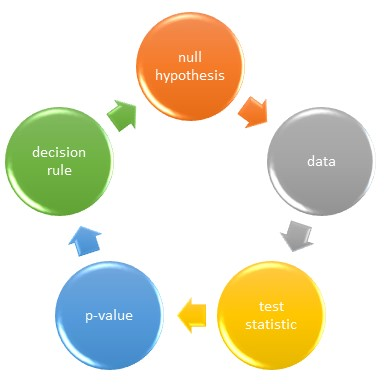
\includegraphics[width=5.33in]{images/hypothesis} \caption{Statistical hypotheses test the null in a multistep process}\label{fig:unnamed-chunk-12}
\end{figure}

Low p-values are associated with extreme values of a test statistic. Extreme values of test statistics happen when the effect sizes of the results are high. Rejecting a null on the basis of a p-value means our test statistic value is too extreme to belong in the distribution of null test statistic values.

Thus, a low p-value means the effect size is improbably high if it were, in fact, not truly effective.

If you learn nothing more in this course, learn that the statistics discussed here are tests of the null hypothesis. Learn that every p-value you see in R output is coupled to a test statistic value. These p-values represent the probability your evidence belongs in the null test statistic distribution.

\hypertarget{popper-and-falsification}{%
\section{Popper and falsification}\label{popper-and-falsification}}

Using data to falsify an hypothesis, even if that hypothesis is the null, is a decision framework that plays well with philosopher Karl Popper's assertion that \href{https://plato.stanford.edu/entries/popper/\#ProbDema}{scientific theories are probative} and that unscientific theories are not.

To Popper, the grandest scientific theories are those that can be falsified. In Popperian logic, the truth of nature is unknowable and unproveable\ldots{}.even though it is testable. Thus, the scientific method advocated by Popper doesn't allow for proving an hypothesis, but at the same time it doesn't forbid us from rejecting hypotheses that are inconsistent with observations.

Thus enters the null hypothesis, which predicts, of course, that nothing happens. The null is an incredibly handy device because if we make observations that are extremely inconsistent with the null, meaning we have observed that something happens, we are obligated to reject the null. Thus, the null is falsifiable when we have positive results!

Imagine an experiment to test whether a drug lowers blood glucose in people who have diabetes. When the glucose-lowering effect size for the drug in the sample is large enough, we can reject the hypothesis that the drug didn't have any effect.

In other words, we will accept an observation as evidence for a positive result by formally concluding that same evidence is inconsistent with a negative result.

Some argue that this logic forces the researcher to test the ``wrong'' hypothesis and to also accept an alternate hypothesis that itself may not be true. For example, although blood glucose may be lower in the drug treatment arm of the sample, that may have occured by random chance. An unknown confounder variable could be responsible for the observation that drug-treatment is associated with lower blood glucose.

In that case we would make an error by rejecting the null when it is actually true.

Of course, rejecting the null is provisional. All gained knowledge is provisional. Drawing a conclusion from one experiment doesn't preclude testing the experiment some other way. If the problem is important enough (and ``real''), it will be tested from multiple angles. It will need to survive the preponderance of the evidence.

I'm convinced the alternative approach, which is to seek out evidence that affirms an hypothesis, is not better. This lies at the heart of what Popper stood against. There is an inherent confirmation bias in seeking out affirmation of ideas. In the proper light, any evidence can be made to look attractive. Furthermore, what if, in seeking affirmation, nothing happens? Negative results are very difficult to interpret because the absence of evidence cannot be interpreted as the evidence of absence.

So I'd hope the researcher who gives this some thought will find null falsification more pragmatic, if not ingenious. It allows us to move forward on the basis of positive evidence (granted, which may be wrong and we don't know it), while at the same time practicing a more sound, more unbiased scientific methodology (hypothesis falsification rather than affirmation).

Meanwhile, this statistical framework does allow for the possibility of designing experimental conditions to minimize false positive (type1) and false negative (type2) errors. We can operationalize our tolerance for those kinds of mistakes in meaningful ways such that we are less likely to become victims of bad luck.

Finally, the decision to reject a null hypothesis can stand alone. It need not be the same as a decision to accept the alternate. Rejecting the null only asserts that the experimental evidence is inconsistent with the null. In no way does that ``prove''" the alternative hypothesis.

For most, some of these concerns should become even less of a problem when the null and alternate hypotheses are explicitly framed in terms of population parameters and their \textbf{mutually exclusive and collectively exhaustive} outcomes. This approach doesn't leave much room for ambiguity about what is being declared at the decision step.

For example, the null hypothesis for the diabetes case is very explicit: \(null, H_0: \mu_{placebo} = \mu_{drug}\), Here \(\mu\), since it is greek notation, represents the mean blood glucose in concentration units in the populations corresponding to the two sampled groups.

Now that we have a bona fide null hypothesis, we can state the alternate hypothesis as everything the null can't be: \(alternate, H_1: \mu_{placebo}\ \ne \mu_{drug}\)

In other words, the inference operates on the basis of straightforward mathematical principles. Two parameters that are compared either meet our prescribed expectations, or they do not. In this case, if we reject the hypothesis that the means of the two groups are equal, then they can only be not equal.

Are they truly not equal? We can never know for sure, but we are operating within a framework of known error tolerances.

\hypertarget{statistical-hypothesis-rubric}{%
\section{Statistical hypothesis rubric}\label{statistical-hypothesis-rubric}}

Researchers have to grapple with two types of hypotheses. One type is the grand, paradigm-driving assertion of some key insight, which is designed to express the big picture in forward thinking terms. It is also designed to wow study sections and seminar audiences.

The other type is the null hypothesis, which is designed to be tested statistically. The null predicts nothing will happen. The null is as boring as it gets. You'd never propose the null in a specific aims page, but you should get in the habit of thinking in terms of testing the null with your statistics.

Only the null hypothesis has any statistical utility, whereas the grand hypothesis has no statistical utility. This is a conceptual hurdle that most students struggle with. The grand hypothesis is for marketing, the null hypothesis is for mattering.

For that reason I've created a rubric for forming a statistically testable hypothesis. The rubric begins with a conceptual overview of a problem, and it ends with how the results will be interpreted. At some point during the semester you'll have a major assignment that asks you to go through this rubric for a problem of your own choosing. That assignment is a major test for whether you ``get'' statistical design of experiments.

\textbf{Step 1: Lay out the big picture of the problem in a way that leads to a ``What is not yet known'' assertion.}

\emph{Type 2 diabetes is associated with high blood glucose levels and obesity, which each have long term effects associated with high morbidity. Exenatide is GLP-1 receptor agonist that can control blood glucose levels. When delivered as an osmotic minipump exenatide lowers blood glucose. A standard of care for type2 diabetics is to put them on a weight loss program while giving them drugs that manage blood glucose. It is not known if continuous administration via osmotic minipump can lead to greater weight loss while on this standard of care.}

\textbf{Step 2: Transform the ``What is not known'' statement into a bold and simple scientific prediction, as if ``what is not known'' were answered:}

\emph{Long-term administration of exenatide via osmotic minipump to type-2 diabetics will cause weight loss.}

\textbf{Step 3: Now frame the experimental plan in terms of the independent and dependent variables, written as an if/then statement. In narrative format, if you manipulate what predictor variables, then what outcome do you expect to observe?}

\emph{If an exenatide osmotic minipump is implanted into type-2 diabetics, then their weight loss will differ compared to placebo.}

\textbf{Step 4: Define the dependent and the independent variables of the experiment. What type of variables are these? What are the experimental units? Are the measurements intrinsically-linked, or not?}

\emph{The dependent variable will be weight loss, calculated as the weight difference between pre-study to post-study for each human subject. Each subject is the experimental unit. The independent variable is treatment. Treatment is a discrete, factoral variable that will be at two levels, placebo and exenatide. Although pre- and post-study weights will be measured for each subject and are themselves intrinsically-linked, they are used to derive the dependent variable (weight loss), which are not instrinsically-linked.}

\textbf{Step 5: Write the null and alternate hypothesis on the basis of the statistical parameters to be tested. Note here that greek notation is used to symbolize that the hypothesis is about the sampled population parameters, rather than the sample.}

\emph{Where} \(\mu\) \emph{represents the mean weight loss of the populations corresponding to the sampled groups, the null and alternate hypotheses are} \[H_0:\mu_{exenatide}=\mu_{placebo}\] \emph{and} \[H_1: \mu_{exenatide}\ne\mu_{placebo}\]

\textbf{Step 6: What statistical test will be used to test the null hypothesis? What are the decision rules?}

\emph{A two-sided, unpaired t-test for comparing group means. The sample size will be based upon a power of 90\%, which means that the tolerance level for type2 error will be 10\%. The decision threshold for type1 error will be 5\%. Thus, the null hypothesis will be rejected at a p-value of less than 0.05.}

\hypertarget{two-sided-vs-one-sided-hypothesis}{%
\subsubsection{Two-sided vs one-sided hypothesis}\label{two-sided-vs-one-sided-hypothesis}}

The above is an example for a two-sided hypothesis. In a two-sided hypothesis \(\ne\) is mutually exclusive and collectively exhaustive of \(=\). By rejecting the null that two things are equal, we implicitly (and provisionally) accept the alternative hypothesis that they are not equal.

Notice how this hypothesis doesn't predict the direction of an effect. It only predicts there will be a difference between the two groups.

If you're willing to predict the direction of an effect, you would choose to make a one-sided hypothesis.

One-sided hypotheses can happen in either of two ways. In one case we can predict one mean will be greater (\(>\))than another mean. In the other case, we can predict one mean will be less than (\(<\)) another mean. The mutually exclusive and collectively exhaustive alternatives to these one sided hypotheses are therefore \(\ge\) and \(\le\), respectively. In other words, if one mean is not greater than another mean, then the only alternative possibilities are that it is less than or equal to it.

The decision to test a one- or two-sided hypothesis should be based upon scientific reasoning.

In the example above, I'm unwilling to test a one-sided hypothesis that exenatide will cause a greater weight loss than placebo, even though that is the expectation (and hope!). Were I willing to test the direction of the effect, the one-sided hypothesis test would be written like this:

\[H_0:\mu_{exenatide}<\mu_{placebo}\] \emph{and} \[H_1: \mu_{exenatide}\ge\mu_{placebo}\]

If the data show that mean weight loss is greater in the exenatide group, as expected, that null hypothesis can be rejected.

But what if, unexpectedly, weight loss is greater in the placebo group? It would generate a high p-value. According to the pre-planned hypothesis, the null could not be rejected.

Worse, given they are already enrolled in a standard of care weight loss program, to know the drug actually impairs weight loss would be an important finding. But in choosing the incorrect one-sided hypothesis, there is nothing to do with the result. It is a negative result. I can't flip the tail to the other direction to get a significant result that I wasn't planning upon. That would be extremely biased!

In practice, some researchers caught in this conundrum create a whole new can of worms by simply changing the pre-planned hypothesis after the fact. It's done flippantly but is actually a fairly serious violation of scientific integrity. Changing the hypothesis so that it is consistent with the results is not what anybody would consider sound scientific method.

\hypertarget{stick-to-two-sided-hypotheses}{%
\subsubsection{Stick to two-sided hypotheses}\label{stick-to-two-sided-hypotheses}}

Unlike the case above, when being wrong about the direction of an effect is not a big deal, then one-sided tests are not a bad option.

The example above serves to illustrate how a two-sided hypothesis would have been a better choice than a one-sided hypothesis. There are a few other reasons why it is probably better to get in the habit of always testing two-sided nulls: the two-sided test is more conservative because the p-value threshold is a bit lower. Furthermore, multiple tests and confidence intervals easier perform and to interpret, respectively.

\hypertarget{error}{%
\chapter{Error}\label{error}}

\begin{Shaded}
\begin{Highlighting}[]
\KeywordTok{library}\NormalTok{(tidyverse)}
\KeywordTok{library}\NormalTok{(treemapify)}
\KeywordTok{library}\NormalTok{(pwr)}
\end{Highlighting}
\end{Shaded}

In a jury trial under the American system of justice the defendant stands accused of a crime by a prosecutor. Both sides present evidence before a jury. The jury's duty is to weigh the evidence then vote in favor of or against a conviction.

The jury doesn't know the truth.

A jury is at risk of making two types of mistakes: An innocent person might be convicted, or a guilty person might be acquitted. They can also make two correct calls: Convict a guilty person or acquit someone who is innocent.

Without ever knowing for sure what is actually true, they are instructed by the judge to record their decision on the basis of a threshold rule. In a trial the rule is vote to convict only when you believe ``it is beyond a reasonable doubt'' the accused is guilty.

In science the researcher is like a jury. The experiment is like a trial. At the end, the researcher has the same problem that jurors face. There is a need to conclude whether the experiment worked or not. And there's no way to know with absolute certainty. Mistaken judgments are possible.

Whereas the jury works within the ``beyond a reasonable doubt'' framework, researchers operate within a framework that establishes tolerance limits for error.

Every hypothesis tested risks two types of error. A type 1 error is committed when the researcher rejects the null when in fact there is no effect. This is also known as a false positive. A type 2 error is not rejecting the null when it should be rejected, which is known as a false negative.

Or the researcher might not make an error at all. The sensitivity of an experiment is conclude correctly there is no effect, and power (also known as specificity) is concluding correctly there is an effect. Sensitivity and power are the complements of type 1 and type 2 error, respectively

\hypertarget{setting-type-1-and-type-2-error-thresholds}{%
\section{Setting type 1 and type 2 error thresholds}\label{setting-type-1-and-type-2-error-thresholds}}

In the planning stages of an experiment the researcher establishes tolerance for these errors. A balance has to be struck between aversion for each error type, the ability to make the right call, and the costs involved for being either wrong or right.

\hypertarget{setting-alpha-the-type-1-error}{%
\subsection{Setting alpha-the type 1 error}\label{setting-alpha-the-type-1-error}}

In the biological sciences the standard for type 1 error is 5\%, meaning in any given experiment (no matter the number of comparisons to be made), the chance of generating a false positive should be limited to 5\%.

The acceptable type 1 error limit is labeled alpha, or \(\alpha\). In several R statistical functions, it is controlled by adjusting its complement, the confidence level.

Why is \(\alpha\) 5\% and not some other value? Credit for that is owed largely to R.A. Fisher who offered that a 1 in 20 chance of making such a mistake seemed reasonable. That number seems to have stuck, at least in the biological sciences.

The researcher is always free to establish, and defend, some other level of \(\alpha\). In the field of psychology, for example, \(\alpha\) is historically 10\%.

There is nothing to stop a researcher from selecting a threshold below or above 5\%. She just needs to be prepared to defend the choice.

\hypertarget{the-decision-rule}{%
\subsubsection{The decision rule}\label{the-decision-rule}}

The \(\alpha\) is stated before an experiment begins, but operationalized during the final statistical analysis on the basis of p-values generated from statistical tests. \textbf{The null hypothesis is rejected when a p-value is less than this preset \(\alpha\).}

\hypertarget{experimentwise-error}{%
\subsubsection{Experimentwise error}\label{experimentwise-error}}

An experiment that just compares two groups (eg, placebo vs drug) generates only one hypothesis. An experiment comparing \(k\) groups (eg, placebo vs drug1, vs drug2\ldots{}drugk-1) generates \(m=\frac{k(k-1)}{2}\) hypotheses.

For experiments that generate multiple hypotheses it is important to maintain the overall \(\alpha\) for the experiment at 5\%. If not checked, the experiment-wise error would inflate with each hypothesis tested.

Several methods have been devised to maintain experiment-wise \(\alpha\) for multiple comparisons. The most conservative of these is the Bonferroni correction \(\alpha_m=\frac{\alpha}{m}\). Thus, if \(m = 10\) hypotheses are tested, the adjusted threshold for each, \(\alpha_m\), is 0.5\%, or a p-value of 0.005. If 1000 hypotheses are tested, such as in a mini-gene screen, the p-value threshold for each would be 0.00005.

\hypertarget{power-setting-beta-the-type-2-error}{%
\subsection{Power: Setting beta-the type 2 error}\label{power-setting-beta-the-type-2-error}}

In the biological sciences the tolerance for type 2 error, otherwise symbolized as \(\beta\), is generally in the neighborhood of 20\%.

It's a bit easier to discuss \(\beta\) through its complement, \(1-\beta\) or power. Thus, experiments run at 80\% power, which are generally regarded as well-designed, run at 20\% risk of type 2 error.

Operationally, an experiment is designed to hit a specific level of power via planning of the sample size. ``Power calculations'' return sample size by integrating intended power, \(\alpha\), and an estimated effect size.

Students tend to fret over effect size estimates. They are nothing more than a best guess of what to expect. A crude estimate. The researcher should use values representing a minimum for a scientific meaningful effect size. The effect size is estimated on the basis of scientific judgment and preliminary data or published information.

If the effect size estimate turns out to be accurate, an experiment run at that sample size should be close to the intended power.

In a perfect world, we might consider powering up every experiment to 99\%, completely minimizing the risk of \(\beta\). As you'll see in the simulation below, the incremental gain in power beyond \textasciitilde{}80\% diminishes with sample size. In other words, perfect power and very low \(\beta\) comes at a high cost. The choice of what power to run an experiment should strike the right balance between the risk of missing out on a real effect against the cost burden of additional resources and time.

R's \texttt{pwr} package has a handful of functions to run power calculations for given statistical tests. These, unfortunately, do not cover all of the statistical tests, particularly for the most common experimental designs (eg, ANOVA).

In this course, we'll emphasize performing power calculations using custom Monte Carlo functions, which can be custom adapted for any type of experiment involving a statistical test.

Here's a custom Monte Carlo-based power function for a t-test. To illustrate the diminishing returns argument, the function calculates power comparing samples drawn from \(N(0,1)\) to samples drawn from \(N(1,1)\). The graph is generated by passing a range of sample sizes into the function. Note how the gain in power plateaus.

\begin{Shaded}
\begin{Highlighting}[]
\NormalTok{t.pwr <-}\StringTok{ }\ControlFlowTok{function}\NormalTok{(n)\{}
  \CommentTok{#Intitializers. Means and SD's of populations compared.}
\NormalTok{  m1=}\DecValTok{1}\NormalTok{; sd1=}\DecValTok{1}\NormalTok{; m2=}\StringTok{ }\DecValTok{0}\NormalTok{; sd2=}\DecValTok{1}
  \CommentTok{# the monte carlo}
\NormalTok{  ssims=}\DecValTok{1000}
\NormalTok{  p.values <-}\StringTok{ }\KeywordTok{c}\NormalTok{()}
\NormalTok{  i <-}\StringTok{ }\DecValTok{1}
  \ControlFlowTok{repeat}\NormalTok{\{}
\NormalTok{    x=}\KeywordTok{rnorm}\NormalTok{(n, m1, sd1); }
\NormalTok{    y=}\KeywordTok{rnorm}\NormalTok{(n, m2, sd2);}
\NormalTok{    p <-}\StringTok{ }\KeywordTok{t.test}\NormalTok{(x, y, }
                \DataTypeTok{paired=}\NormalTok{F, }
                \DataTypeTok{alternative=}\StringTok{"two.sided"}\NormalTok{, }
                \DataTypeTok{var.equal=}\NormalTok{F,}
                \DataTypeTok{conf.level=}\FloatTok{0.95}\NormalTok{)}\OperatorTok{$}\NormalTok{p.value}
\NormalTok{    p.values[i] <-}\StringTok{ }\NormalTok{p}
    \ControlFlowTok{if}\NormalTok{ (i}\OperatorTok{==}\NormalTok{ssims) }\ControlFlowTok{break}
\NormalTok{    i =}\StringTok{ }\NormalTok{i}\OperatorTok{+}\DecValTok{1}
\NormalTok{    pwr <-}\StringTok{ }\KeywordTok{length}\NormalTok{(}\KeywordTok{which}\NormalTok{(p.values}\OperatorTok{<}\FloatTok{0.05}\NormalTok{))}\OperatorTok{/}\NormalTok{ssims}
\NormalTok{  \}}
  \KeywordTok{return}\NormalTok{(pwr)}
\NormalTok{\}}
\CommentTok{#Run t.pwr over a range of sample sizes and plot results}
\NormalTok{frame <-}\StringTok{ }\KeywordTok{data.frame}\NormalTok{(}\DataTypeTok{n=}\DecValTok{2}\OperatorTok{:}\DecValTok{50}\NormalTok{)}
\NormalTok{data <-}\StringTok{ }\KeywordTok{bind_cols}\NormalTok{(frame, }
                  \DataTypeTok{power=}\KeywordTok{apply}\NormalTok{(frame, }\DecValTok{1}\NormalTok{, t.pwr))}
\CommentTok{#plot}
\KeywordTok{ggplot}\NormalTok{(data, }\KeywordTok{aes}\NormalTok{(n, power))}\OperatorTok{+}
\StringTok{  }\KeywordTok{geom_point}\NormalTok{() }\OperatorTok{+}
\StringTok{  }\KeywordTok{scale_y_continuous}\NormalTok{(}\DataTypeTok{breaks=}\KeywordTok{c}\NormalTok{(}\KeywordTok{seq}\NormalTok{(}\DecValTok{0}\NormalTok{, }\DecValTok{1}\NormalTok{, }\FloatTok{0.1}\NormalTok{)))}\OperatorTok{+}
\StringTok{  }\KeywordTok{scale_x_continuous}\NormalTok{(}\DataTypeTok{breaks=}\KeywordTok{c}\NormalTok{(}\KeywordTok{seq}\NormalTok{(}\DecValTok{0}\NormalTok{,}\DecValTok{50}\NormalTok{,}\DecValTok{2}\NormalTok{)))}\OperatorTok{+}
\StringTok{  }\KeywordTok{labs}\NormalTok{(}\DataTypeTok{x=}\StringTok{"n per group"}\NormalTok{)}
\end{Highlighting}
\end{Shaded}

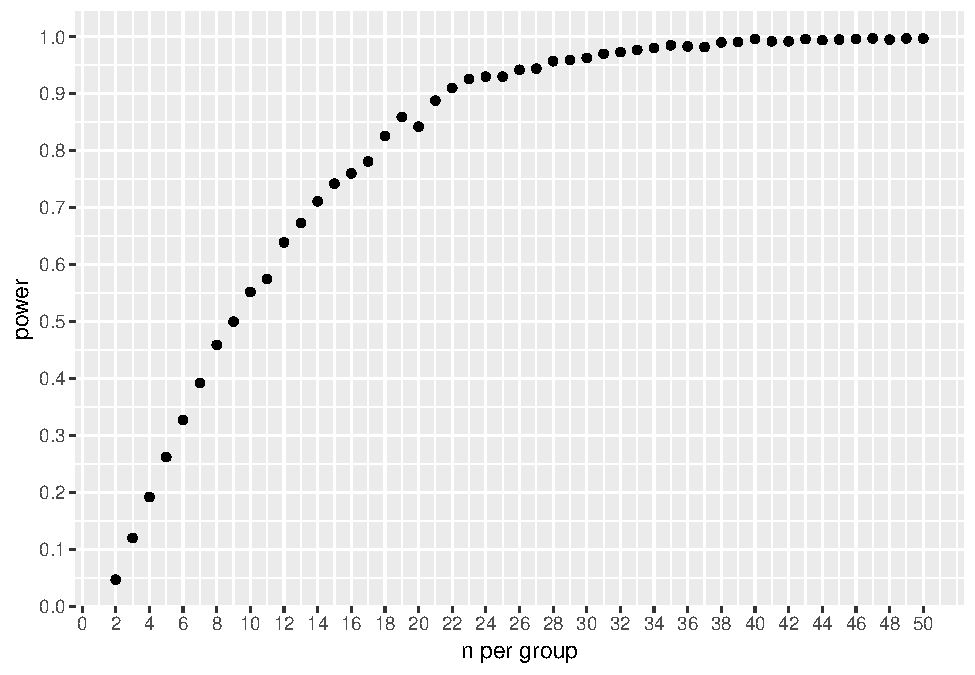
\includegraphics{jabstb_files/figure-latex/unnamed-chunk-14-1.pdf}

\begin{Shaded}
\begin{Highlighting}[]
\CommentTok{## Validation by comparisonC to pwr package results}
\KeywordTok{pwr.t.test}\NormalTok{(}\DataTypeTok{d=}\DecValTok{1}\NormalTok{, }
           \DataTypeTok{sig.level=}\FloatTok{0.05}\NormalTok{, }
           \DataTypeTok{power=}\FloatTok{0.8}\NormalTok{, }
           \DataTypeTok{type=}\StringTok{"two.sample"}\NormalTok{)}
\end{Highlighting}
\end{Shaded}

\begin{verbatim}
## 
##      Two-sample t test power calculation 
## 
##               n = 16.71472
##               d = 1
##       sig.level = 0.05
##           power = 0.8
##     alternative = two.sided
## 
## NOTE: n is number in *each* group
\end{verbatim}

\hypertarget{striking-the-right-balance}{%
\section{Striking the right balance}\label{striking-the-right-balance}}

The script below provides a way to visualize how the relationship between correct (green) and incorrect (red) decisions varies with error thresholds.

The idea is to run experiments under conditions by which green is the dominant color.

Unfortunately, most published biomedical research appears to be \href{https://www.ncbi.nlm.nih.gov/pmc/articles/PMC5367316/}{severely underpowered findings}.

\begin{Shaded}
\begin{Highlighting}[]
\NormalTok{alpha <-}\StringTok{ }\FloatTok{0.05}
\NormalTok{beta <-}\StringTok{ }\FloatTok{0.20}

\NormalTok{panel <-}\StringTok{ }\KeywordTok{data.frame}\NormalTok{(alpha, }
                    \DataTypeTok{sensitivity=}\DecValTok{1}\OperatorTok{-}\NormalTok{alpha, }
                    \DataTypeTok{power=}\DecValTok{1}\OperatorTok{-}\NormalTok{beta, }
\NormalTok{                    beta)}
\NormalTok{panel <-}\StringTok{ }\KeywordTok{gather}\NormalTok{(panel, }\DataTypeTok{key=}\StringTok{"threshold"}\NormalTok{, }
         \DataTypeTok{value=}\StringTok{"percent"}\NormalTok{) }

\NormalTok{panel <-}\StringTok{ }\KeywordTok{bind_cols}\NormalTok{(panel, }
                   \DataTypeTok{truth=}\KeywordTok{c}\NormalTok{(}\StringTok{"no effect"}\NormalTok{, }\StringTok{"no effect"}\NormalTok{, }\StringTok{"effective"}\NormalTok{, }\StringTok{"effective"}\NormalTok{), }
                   \DataTypeTok{decision=}\KeywordTok{c}\NormalTok{(}\StringTok{"effective"}\NormalTok{, }\StringTok{"no effect"}\NormalTok{, }\StringTok{"effective"}\NormalTok{, }\StringTok{"no effect"}\NormalTok{), }
                   \DataTypeTok{choice=}\KeywordTok{c}\NormalTok{(}\StringTok{"error"}\NormalTok{, }\StringTok{"correct"}\NormalTok{, }\StringTok{"correct"}\NormalTok{, }\StringTok{"error"}\NormalTok{))}
\NormalTok{panel}
\end{Highlighting}
\end{Shaded}

\begin{verbatim}
##     threshold percent     truth  decision  choice
## 1       alpha    0.05 no effect effective   error
## 2 sensitivity    0.95 no effect no effect correct
## 3       power    0.80 effective effective correct
## 4        beta    0.20 effective no effect   error
\end{verbatim}

\begin{Shaded}
\begin{Highlighting}[]
\KeywordTok{ggplot}\NormalTok{(panel, }\KeywordTok{aes}\NormalTok{(}\DataTypeTok{area=}\NormalTok{percent, }\DataTypeTok{fill=}\NormalTok{choice, }\DataTypeTok{label=}\NormalTok{threshold))}\OperatorTok{+}
\StringTok{  }\KeywordTok{geom_treemap}\NormalTok{(}\DataTypeTok{color=}\StringTok{"white"}\NormalTok{)}\OperatorTok{+}
\StringTok{  }\KeywordTok{geom_treemap_text}\NormalTok{(}
    \DataTypeTok{fontface =} \StringTok{"italic"}\NormalTok{,}
    \DataTypeTok{colour =} \StringTok{"white"}\NormalTok{,}
    \DataTypeTok{place =} \StringTok{"centre"}\NormalTok{,}
    \DataTypeTok{grow =}\NormalTok{ F}
\NormalTok{  )}\OperatorTok{+}
\StringTok{  }\KeywordTok{scale_fill_manual}\NormalTok{(}\DataTypeTok{values =} \KeywordTok{alpha}\NormalTok{(}\KeywordTok{c}\NormalTok{(}\StringTok{"green3"}\NormalTok{, }\StringTok{"red"}\NormalTok{), }\FloatTok{.3}\NormalTok{))}
\end{Highlighting}
\end{Shaded}

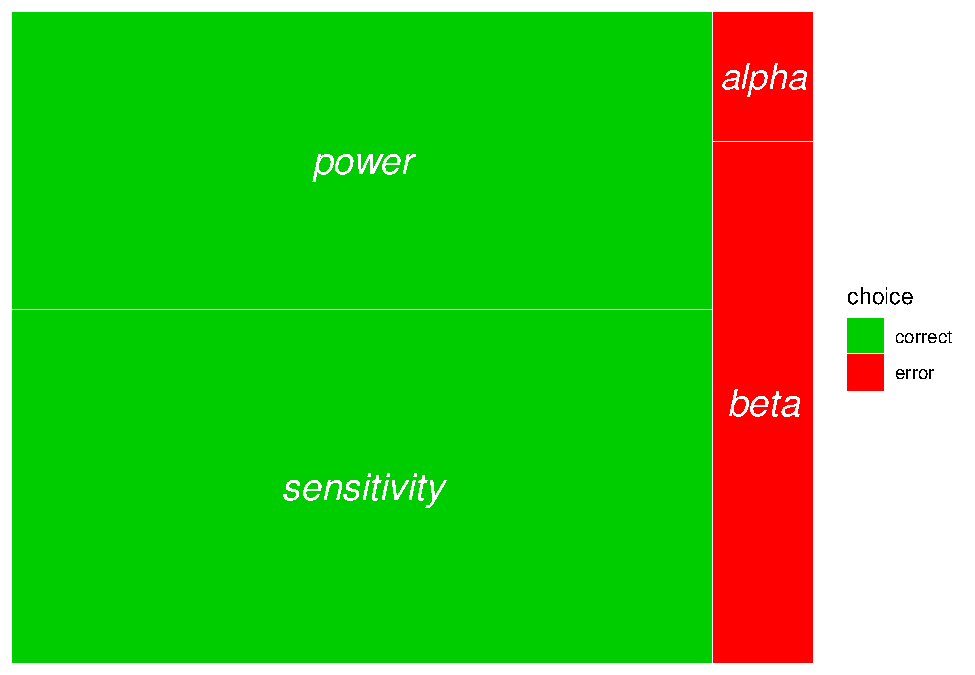
\includegraphics{jabstb_files/figure-latex/unnamed-chunk-15-1.pdf}

\hypertarget{false-discovery-rate}{%
\section{False discovery rate}\label{false-discovery-rate}}

The false discover rate, or FDR is another way to estimate experimental error.
\[FDR=\frac{false\ positives}{false\ positives + false\ negatives}\]

FDR varies given \(\alpha\), \(\beta\) and \href{http://rsos.royalsocietypublishing.org/content/1/3/140216}{the probability of the effect}. The probability of the effect bears some comment. Think of it as a prior probability, or the likelihood that an effect being studied is ``real''. It takes some scientific judgment to estimate these probability values.

The graph below illustrates how FDR inflates, particularly when running experiments for low probability effects when tested at low power, even at a standard \(\alpha\).

These relationships clearly show that the lower the likelihood of some effect that you would like to test in an experiment, the higher the stringency by which it should be tested.

\begin{Shaded}
\begin{Highlighting}[]
\NormalTok{px <-}\StringTok{ }\KeywordTok{seq}\NormalTok{(}\FloatTok{0.1}\NormalTok{, }\FloatTok{1.0}\NormalTok{, }\FloatTok{0.1}\NormalTok{) }\CommentTok{#a range of prior probabilities}
\NormalTok{tests <-}\StringTok{ }\DecValTok{10000}
\NormalTok{fdr_gen <-}\StringTok{ }\ControlFlowTok{function}\NormalTok{(beta, alpha)\{}
\NormalTok{  real_effect <-}\StringTok{ }\NormalTok{px}\OperatorTok{*}\NormalTok{tests}
\NormalTok{  true_pos <-}\StringTok{ }\NormalTok{real_effect}\OperatorTok{*}\NormalTok{(}\DecValTok{1}\OperatorTok{-}\NormalTok{beta)}
\NormalTok{  false_neg <-}\StringTok{ }\NormalTok{real_effect}\OperatorTok{*}\NormalTok{beta}
\NormalTok{  no_effect <-}\StringTok{ }\NormalTok{tests}\OperatorTok{*}\NormalTok{(}\DecValTok{1}\OperatorTok{-}\NormalTok{px)}
\NormalTok{  true_neg <-}\StringTok{ }\NormalTok{tests}\OperatorTok{*}\NormalTok{(}\DecValTok{1}\OperatorTok{-}\NormalTok{alpha)}
\NormalTok{  false_pos <-}\StringTok{ }\NormalTok{no_effect}\OperatorTok{*}\NormalTok{alpha}
\NormalTok{  FDR <-}\StringTok{ }\NormalTok{false_pos}\OperatorTok{/}\NormalTok{(true_pos }\OperatorTok{+}\StringTok{ }\NormalTok{false_pos)}
  \KeywordTok{return}\NormalTok{(FDR)}
\NormalTok{\}}
\NormalTok{upss <-}\StringTok{ }\KeywordTok{fdr_gen}\NormalTok{(}\FloatTok{0.6}\NormalTok{, }\FloatTok{0.05}\NormalTok{)}\CommentTok{#under-powered, standard specificity}
\NormalTok{wpss <-}\StringTok{ }\KeywordTok{fdr_gen}\NormalTok{(}\FloatTok{0.2}\NormalTok{, }\FloatTok{0.05}\NormalTok{)}\CommentTok{#well-powered, standard specificity}
\NormalTok{uphs <-}\StringTok{ }\KeywordTok{fdr_gen}\NormalTok{(}\FloatTok{0.6}\NormalTok{, }\FloatTok{0.01}\NormalTok{)}\CommentTok{#under-powered, high specificity}
\NormalTok{wphs <-}\StringTok{ }\KeywordTok{fdr_gen}\NormalTok{(}\FloatTok{0.2}\NormalTok{, }\FloatTok{0.01}\NormalTok{)}\CommentTok{#well-powered, high specificity}
\NormalTok{fdrates <-}\StringTok{ }\KeywordTok{data.frame}\NormalTok{(px,upss, wpss, uphs, wphs)}
\KeywordTok{colnames}\NormalTok{(fdrates) <-}\StringTok{ }\KeywordTok{c}\NormalTok{(}\StringTok{"Probability"}\NormalTok{,}
                       \StringTok{"5% alpha, 60% beta"}\NormalTok{, }
                       \StringTok{"5% alpha, 20% beta"}\NormalTok{, }
                       \StringTok{"1% alpha, 60% beta"}\NormalTok{, }
                       \StringTok{"1% alpha, 20% beta"}\NormalTok{)}

\CommentTok{#convert to long format}
\NormalTok{fdrates <-}\StringTok{ }\KeywordTok{gather}\NormalTok{(fdrates, tests, FDR, }\OperatorTok{-}\NormalTok{Probability)}
\KeywordTok{ggplot}\NormalTok{(fdrates, }\KeywordTok{aes}\NormalTok{(Probability,FDR, }\DataTypeTok{group=}\NormalTok{tests))}\OperatorTok{+}
\StringTok{  }\KeywordTok{geom_point}\NormalTok{(}\KeywordTok{aes}\NormalTok{(}\DataTypeTok{color=}\KeywordTok{factor}\NormalTok{(tests)))}\OperatorTok{+}
\StringTok{  }\KeywordTok{geom_line}\NormalTok{(}\KeywordTok{aes}\NormalTok{(}\DataTypeTok{color=}\KeywordTok{factor}\NormalTok{(tests)))}
\end{Highlighting}
\end{Shaded}

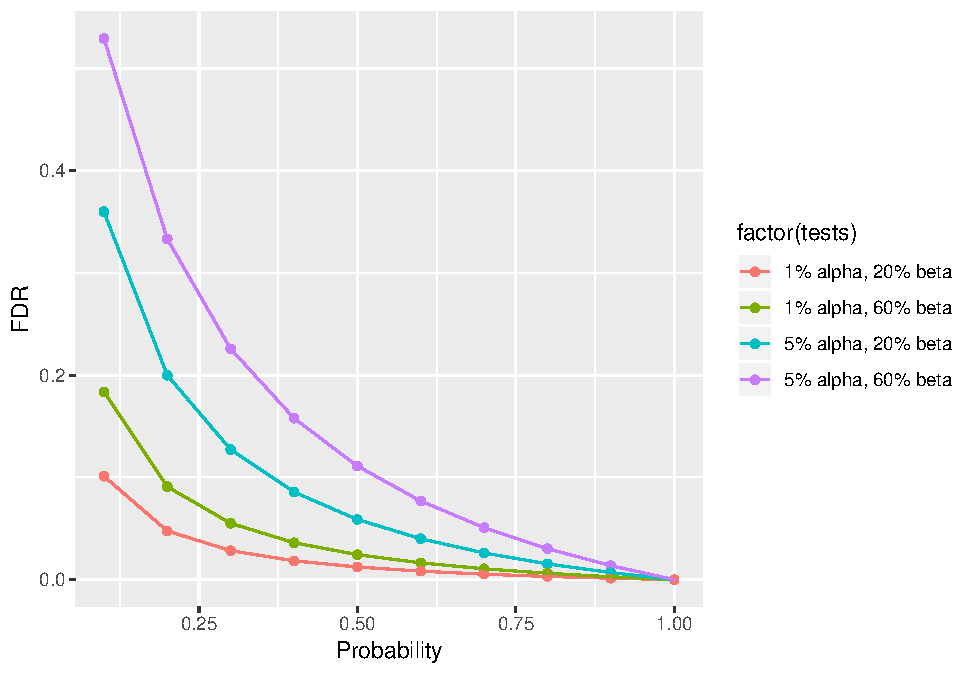
\includegraphics{jabstb_files/figure-latex/unnamed-chunk-16-1.pdf}

\hypertarget{pvalues}{%
\chapter{P Values}\label{pvalues}}

\begin{Shaded}
\begin{Highlighting}[]
\KeywordTok{library}\NormalTok{(tidyverse)}
\end{Highlighting}
\end{Shaded}

You'll see soon enough that when you run a statistical test function in R, it generates list objects that are chock full of useful information.

Invariably, the researcher's eyes will go right to the p-value. This is understandable, since most researchers have been trained to associate their own success with a p-value falling below some pre-set \(\alpha\). Who could really blame them for peeking at the p-values first?

The p-value is an instrument by which an important decision will be made. As such, it is worth understanding how that instrument works.

Hypothesis-driven experiments are designed to test the null hypothesis. That null will be rejected if the effect size is large enough. Extreme effect sizes correspond to extreme values of test statistics.

\textbf{A p-value is the probability that a given test statistic value could be as large as it is, or even more extreme, if the null hypothesis were actually true.}

In other words, the p-value is an error probability. It is also a random variable. Which means that it is always possible for an experiment to generate an extreme test statistic by simple random chance. The p-value asserts the probability that this is the case.

One of the reasons I like using R for experimental statistics is that R makes it easy to simulate p-values. Because of that you build an intuitive sense for how they operate. R makes it easy to understand p-values.

\hypertarget{how-p-values-are-calculated}{%
\section{How p-values are calculated}\label{how-p-values-are-calculated}}

You can think of test statistics as a transformation of sample data. There are many test statistics. The one to use for a given data set depends on the experimental design. Each test statistic has a probability distribution. P-values are derived from the probability distributions of these test statistics and serve as a way to standardize the decision making process irrespective of the experimental design and test statistic.

Probably the simplest test statistic to understand is the z-score. The z-score is a transformation of data from whatever scale it is on, to a standard normal scale. It's usually appropriate for continuous data.
\[z_i=\frac{y_i-\mu}{\sigma}\]
Let's say we have single blood glucose value of 122 mg/dl. What is its p-value? Is the z-score corresponding to that glucose value too extreme to belong in the null distribution of z-scores?

First, the blood glucose values is transformed into a z-score. We'll say the mean and standard deviation of blood glucose in the sampled population is 100 and 10 mg/dl, respectively. The z-score for a value of 122 is therefore:

\begin{Shaded}
\begin{Highlighting}[]
\NormalTok{z <-}\StringTok{ }\NormalTok{(}\DecValTok{122-100}\NormalTok{)}\OperatorTok{/}\DecValTok{10}\NormalTok{; z}
\end{Highlighting}
\end{Shaded}

\begin{verbatim}
## [1] 2.2
\end{verbatim}

z-score units are in standard deviations. Thus, a z-score value of 2.2 indicates it is 2.2 standard deviation units greater than the standard normal mean (which is zero, of course).

Next, we'll pass that z-score value of 2.2 into the standard normal density function, \texttt{pnorm}. We cause the function to produce a p-value for that z-score by using a \texttt{lower.tail=FALSE} argument:

\begin{Shaded}
\begin{Highlighting}[]
\KeywordTok{pnorm}\NormalTok{(}\FloatTok{2.2}\NormalTok{, }\DataTypeTok{mean=}\DecValTok{0}\NormalTok{, }\DataTypeTok{sd=}\DecValTok{1}\NormalTok{, }\DataTypeTok{lower.tail=}\OtherTok{FALSE}\NormalTok{)}
\end{Highlighting}
\end{Shaded}

\begin{verbatim}
## [1] 0.01390345
\end{verbatim}

In the z probability distribution below, the blue shaded region illustrates what this p-value looks like. The p-value covers the probabilities for z-score values of 2.2 and higher. The p-value is thus the area under the curve for the z probability distribution for that value of z and for more extreme values.

\begin{Shaded}
\begin{Highlighting}[]
\KeywordTok{ggplot}\NormalTok{(}\KeywordTok{data.frame}\NormalTok{(}\DataTypeTok{zscore =} \KeywordTok{c}\NormalTok{(}\OperatorTok{-}\DecValTok{5}\NormalTok{, }\DecValTok{5}\NormalTok{)), }\KeywordTok{aes}\NormalTok{(zscore)) }\OperatorTok{+}
\StringTok{  }\KeywordTok{stat_function}\NormalTok{(}\DataTypeTok{fun =}\NormalTok{ dnorm) }\OperatorTok{+}
\StringTok{  }\KeywordTok{stat_function}\NormalTok{(}\DataTypeTok{fun =}\NormalTok{ dnorm,}
                \DataTypeTok{xlim=} \KeywordTok{c}\NormalTok{(}\FloatTok{2.2}\NormalTok{, }\DecValTok{5}\NormalTok{),}
                \DataTypeTok{geom =} \StringTok{"area"}\NormalTok{, }\DataTypeTok{fill=}\StringTok{"blue"}\NormalTok{)}\OperatorTok{+}
\StringTok{  }\KeywordTok{ylab}\NormalTok{(}\StringTok{"p(z)"}\NormalTok{)}\OperatorTok{+}
\StringTok{  }\KeywordTok{scale_x_continuous}\NormalTok{(}\DataTypeTok{breaks=}\KeywordTok{seq}\NormalTok{(}\OperatorTok{-}\DecValTok{5}\NormalTok{,}\DecValTok{5}\NormalTok{,}\DecValTok{1}\NormalTok{))}
\end{Highlighting}
\end{Shaded}

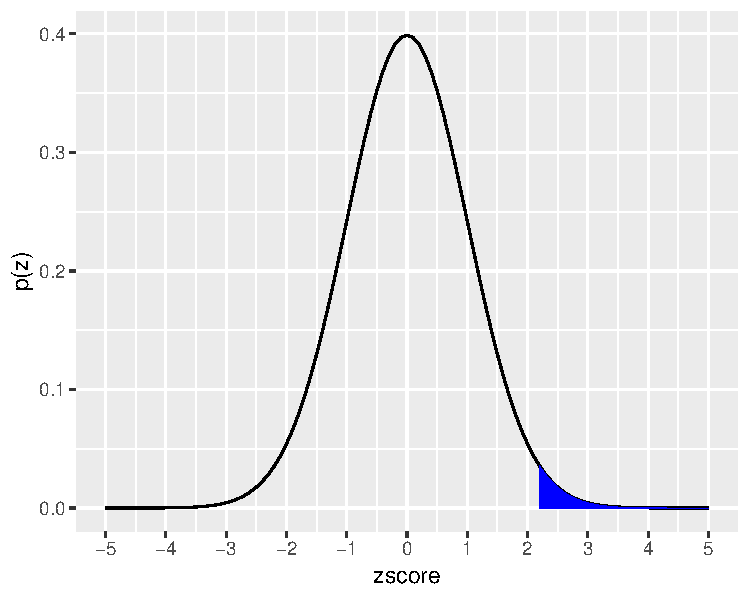
\includegraphics{jabstb_files/figure-latex/unnamed-chunk-20-1.pdf}

\hypertarget{how-p-values-should-be-interpreted}{%
\section{How p-values should be interpreted}\label{how-p-values-should-be-interpreted}}

The question that's ringing in your ears right now is, ``Is a z-score value of 2.2 so extreme we can reject that it belongs to the null distribution of z-scores?''

The answer to that question depends upon what threshold you deem is too extreme. Remember, a threshold is our tolerance for error; in this case, for type 1 error.

If the threshold for an acceptable risk of type 1 error is 5\% (\(p < 0.05\)), then let's see how those look on the z-distribution.

First, let's calculate z-scores corresponding the area outside 95\% of the z-scores. Since extreme z-scores can lay on both the right and the left sides of the z-distribution, which is symmetrical. Therefore we split the 5\% in half and use the quantile function \texttt{qnorm} to calculate z-scores for each:

\begin{Shaded}
\begin{Highlighting}[]
\KeywordTok{qnorm}\NormalTok{(}\FloatTok{0.025}\NormalTok{, }\DataTypeTok{lower.tail =}\NormalTok{ F)}
\end{Highlighting}
\end{Shaded}

\begin{verbatim}
## [1] 1.959964
\end{verbatim}

\begin{Shaded}
\begin{Highlighting}[]
\KeywordTok{qnorm}\NormalTok{(}\FloatTok{0.025}\NormalTok{, }\DataTypeTok{lower.tail =}\NormalTok{ T)}
\end{Highlighting}
\end{Shaded}

\begin{verbatim}
## [1] -1.959964
\end{verbatim}

Thus, the 95\% confidence limits for the z-scores are \textasciitilde{} +/- 1.96, almost 2 standard deviations from the mean. We plug those values as limits into our plot:

\begin{Shaded}
\begin{Highlighting}[]
\KeywordTok{ggplot}\NormalTok{(}\KeywordTok{data.frame}\NormalTok{(}\DataTypeTok{zscore =} \KeywordTok{c}\NormalTok{(}\OperatorTok{-}\DecValTok{5}\NormalTok{, }\DecValTok{5}\NormalTok{)), }\KeywordTok{aes}\NormalTok{(zscore)) }\OperatorTok{+}
\StringTok{  }\KeywordTok{stat_function}\NormalTok{(}\DataTypeTok{fun =}\NormalTok{ dnorm) }\OperatorTok{+}
\StringTok{  }\KeywordTok{stat_function}\NormalTok{(}\DataTypeTok{fun =}\NormalTok{ dnorm,}
                \DataTypeTok{xlim=} \KeywordTok{c}\NormalTok{(}\FloatTok{1.96}\NormalTok{, }\DecValTok{5}\NormalTok{),}
                \DataTypeTok{geom =} \StringTok{"area"}\NormalTok{, }\DataTypeTok{fill=}\StringTok{"red"}\NormalTok{)}\OperatorTok{+}
\StringTok{  }\KeywordTok{stat_function}\NormalTok{(}\DataTypeTok{fun =}\NormalTok{ dnorm,}
                \DataTypeTok{xlim=} \KeywordTok{c}\NormalTok{(}\OperatorTok{-}\FloatTok{1.96}\NormalTok{, }\DecValTok{-5}\NormalTok{),}
                \DataTypeTok{geom =} \StringTok{"area"}\NormalTok{, }\DataTypeTok{fill=}\StringTok{"red"}\NormalTok{)}\OperatorTok{+}
\StringTok{  }\KeywordTok{ylab}\NormalTok{(}\StringTok{"p(z)"}\NormalTok{)}\OperatorTok{+}
\StringTok{  }\KeywordTok{scale_x_continuous}\NormalTok{(}\DataTypeTok{breaks=}\KeywordTok{seq}\NormalTok{(}\OperatorTok{-}\DecValTok{5}\NormalTok{,}\DecValTok{5}\NormalTok{,}\DecValTok{1}\NormalTok{))}
\end{Highlighting}
\end{Shaded}

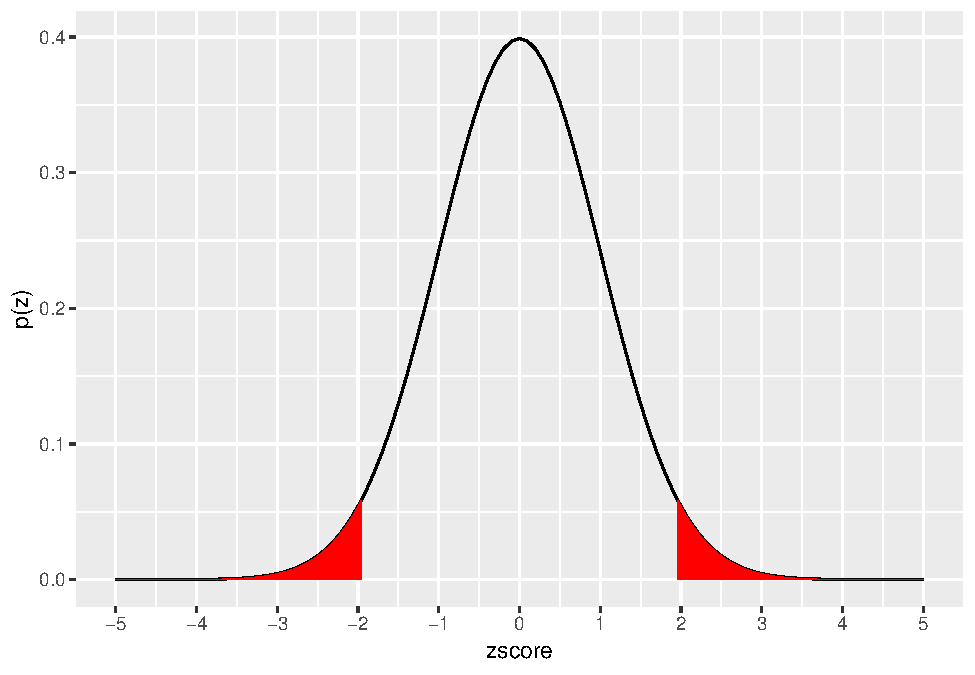
\includegraphics{jabstb_files/figure-latex/unnamed-chunk-22-1.pdf}

Any z-score values corresponding to the red-shaded areas would be deemed too extreme to belong to the null. The limit on the right side is 1.96. Therefore, yes, a z-score of 2.2 (\(p=0.0139\)) is too extreme to belong to the standard null distribution.

\hypertarget{interpretation}{%
\section{Interpretation}\label{interpretation}}

Every time we do an experiment we operate on the assumption that our data represent the null. This is analogous to considering a defendant innocent until proven guilty. So we think of test statistic values we calculate from our data, unless proven otherwise, as belonging to the null distribution of test statistic values.

The interpretation of \(p=0.0139\) is the probability that z-score (and its corresponding glucose value of 122 mg/dl) are that large by chance is 0.0139. There's about a 1.4\% chance we are making an error by rejecting the null that it belongs to the \(N(100, 10)\).

\hypertarget{criticisms-of-p-values}{%
\section{Criticisms of p-values}\label{criticisms-of-p-values}}

There are several criticisms of p-values, many of which are legitimate. I'll address a few key ones here.

\begin{enumerate}
\def\labelenumi{\arabic{enumi}.}
\tightlist
\item
  \emph{They are too confusing, nobody understands them.}
  I get that. I confess that p-values are a struggle to teach in a way that's simple and memorable. Especially for students who only consider statistics episodically, perhaps a few times a year.
\end{enumerate}

This year I'm teaching this with a bit more emphasis upon Popper and the merits of null hypothesis falsification as the cornerstone of the scientific method and how p-values fit into that tradition.

Here it is: All statistical tests (the ones I teach in this course) are tests of the null hypothesis. When the test result is extreme, we reject the null. The p-value is the probability we're rejecting the null in error.

Despite the merit of this particular criticism, p-values are not going away. They are an important inferential tool used by most biological scientists, even if poorly understood and implemented.

Like any tool in the lab, it is incumbant upon the researcher to learn how it works. I think a great way to get a better intuitive understanding for p-values is to play around with the various test statistic probability and quantile distributions in R (\texttt{pnorm,\ qnorm,\ pt,\ qt,\ pf,\ pf,\ pchisq,\ qchisq,\ psignrank,\ qsignrank} etc). Use them to run various scenarios, plot them out\ldots{}get a sense for how the tools work by using them.

\begin{enumerate}
\def\labelenumi{\arabic{enumi}.}
\setcounter{enumi}{1}
\tightlist
\item
  \emph{p-Values poorly protect from false discovery}
  This is undoubtedly true. Since David Colquhoun goes over this in \href{http://rsos.royalsocietypublishing.org/content/1/3/140216}{blistering detail} I won't repeat his thorough analysis here. The researcher MUST operate with skepticism about p-values.
\end{enumerate}

Since Colquhoun's argument is entirely based in simulation it also inspires an approach for dealing with this problem. Through simulation \emph{a priori}, a researcher can design and run experiments \emph{in silico} that strikes the right balance between the threshold levels she can control (eg, \(\alpha\) and \(\beta\)) and feasibility in a way that best minimizes the risk of false discovery. Before ever lifting a finger in the lab.

This criticism explains why I am such a strong advocate of Monte Carlo simulation in experimental design. With software like R, there really is no excuse anymore for the researcher being a victim of this problem.

\begin{enumerate}
\def\labelenumi{\arabic{enumi}.}
\setcounter{enumi}{2}
\tightlist
\item
  \emph{p-Values aren't the probability I'm interested in}
  Researchers who raise this criticism generally are interested in something the p-value was never designed to deliver: the probability that their experiment worked.
\end{enumerate}

A p-value doesn't provide that information because it is an error probability. Specifically, it is the probability of making a type 1 error.

For these researchers, embracing Bayesian statistics is probably a better option. I don't teach Bayesian statistics in this course for a couple of reasons, but mostly because I don't understand it well enough to teach it, and I don't see how it offers a superior approach for experimental research.

\begin{enumerate}
\def\labelenumi{\arabic{enumi}.}
\setcounter{enumi}{3}
\tightlist
\item
  \emph{People use p-values as evidence for the magnitude of an effect.}
  Sure, but they are wrong. This is more a criticism of the people who use p-values, and not the p-value. But the criticism raises the point that it is a mistake to rely solely on a p-value to interpret the outcome of an experiment.
\end{enumerate}

A p-value\textless{}0.05 only means that there is less than 1 out of 20 chance of having detected an extreme effect when the null is true. A low p-value doesn't provide evidence that the treatment effect is real. As a result, a p-value can't provide any information about the magnitude of the treatment effect.

Neither is a low p-value synonymous with scientific significance. A simple example of this comes from 2 way ANOVA F test analysis. When the test suggests a postive result for an interaction effect, that finding supercedes the main effects. Thus, should any main effects also have low p-values they are not scientifically meaningful.

Researchers \href{https://www.nature.com/articles/nmeth.4210}{should therefore analyze p-values in conjunction with other parameters}, such as effect sizes and the confidence intervals.

\hypertarget{data}{%
\chapter{Data Classification}\label{data}}

\begin{Shaded}
\begin{Highlighting}[]
\KeywordTok{library}\NormalTok{(datapasta)}
\KeywordTok{library}\NormalTok{(tidyverse)}
\end{Highlighting}
\end{Shaded}

The starting point in any statistical design is to understand the types of data that are involved. Ask yourself whether the variables are discrete or continuous. Then ask if they measured, ordered or sorted?

If you don't understand those two questions, just read on.

Because the answers will point you in the proper analytical direction.

This is one of the most important things to learn in this course. If you don't get the concept that not all data types are equivalent, you won't get statistics.

In this section data classification will be discussed. In all likelihood this material will sound simplistic or even obvious to you, but I cannot emphasize enough the importance of data classification in mastering a statistical framework.

If for no other reason, understanding how data are classified is crucial in selecting the most appropriate statistical analysis. If you were to approach me to ask, ``here's my stuff, what statistical test should I do?'' I would ask, ``tell me more about your data.'' And we would probably spend a lot of time with you answering my questions until I was sure I understood your data classification.

Therefore, a major learning objective for you is, given a data set, to know which variables are dependent and which are independent, and whether the variables involved are continuous (measured) or discrete (ordered or sorted).

\hypertarget{dependent-and-independent-variables}{%
\section{Dependent and independent variables}\label{dependent-and-independent-variables}}

For the experimental researcher there are two basic types of variables.

An independent variable is the predictor or explanatory variable imposed by the researcher upon a system. Independent variables have values, the levels of which are determined by the researcher. For example, in a blood glucose drug study, the independent variable ``Treatment'' would come in two levels, ``Placebo'' and ``Drug''. In R, we'd call treatment a factor variable with two levels.

Conventionally, the independent variable is plotted on the abcissa, or x-axis, scale of some graph.

A dependent variable is the response or outcome variable collected in an experiment. The values that dependent variables take on are determined by, or dependent upon, the level of the independent variables. For example, the dependent variable in the blood glucose drug study would be a measurement called ``blood\_glucose''.

Most of the time the dependent variable is plotted on the ordinate, or y-axis, scale.

In statistical notation the dependent variable is usually depicted by the uppercase symbol \(Y\). The values that variable can assume are symbolically represented as lowercase symbol \(y_i\), where \(i\) is the sample size, ranging from 1 to \(n\) independent replicates.

Similarly, the indepedent variable is usually depicted by uppercase \(X\) (or some other letter) and its values are lowercase \(x_i\).

I'm going to use that convention but with a twist. Independent variables denoted using \(X\) will represent continuous scaled variables, whereas independent variables denoted using \(A\) or \(B\), or \(C\), will represent discrete, factoral variables. These will take on values denoted by lowercases, eg, \(a_i\), \(b_i\), \(c_i\)) .

To illustrate dependent and independent variables think about a linear relationship between two continuous variables, \(X\) and \(Y\) . This relationship can be expressed using the model \(Y=\beta_0 + \beta_1 X\). \(X\) would be a variable the researcher manipulates, such as time or the concentration of a substance. \(Y\) would be a variable that the researcher measures, such as absorption or binding or fluorescence. The parameters \(\beta_0\) and \(\beta_1\) are constants that modify the relationship between the two variables, which I'm sure you recognize as representing the y-intercept and slope, respectively, of the regression line between the two variables.

Thus, \(Y\) takes on different values as the researcher manipulates the levels of \(X\). Which explains why \(Y\) depends on \(X\).

For example, here's how the data for a protein standard curve experiment would be depicted. In the R script below the variable \(X\) represents known concentrations of an immunoglobulin protein standard in \(\mu g/ml\). The researcher builds this dilution series from a known stock, thus it is the independent variable. The variable \(Y\) represents \(A_{595}\), light absorption in a spectrophotometer for each of the values of the standard protein. The \(A_{595}\) values depend upon the immmunoglobulin concentration. Estimates for \(\beta_0\) and \(\beta_1\) are derived from running a linear regression on the data with the \texttt{lm(Y\textasciitilde{}X)} script. Thus, for every one unit increment in the value of \(X\), there is a 0.02497 increment in the value of \(Y\). Again, \(Y\) depends upon \(X\).

\begin{Shaded}
\begin{Highlighting}[]
\CommentTok{#Protein assay data, X units ug/ml, Y units A595.}
\NormalTok{X <-}\StringTok{ }\KeywordTok{c}\NormalTok{(}\DecValTok{0}\NormalTok{, }\FloatTok{1.25}\NormalTok{, }\FloatTok{2.5}\NormalTok{, }\DecValTok{5}\NormalTok{, }\DecValTok{10}\NormalTok{, }\DecValTok{15}\NormalTok{, }\DecValTok{20}\NormalTok{, }\DecValTok{25}\NormalTok{)}
\NormalTok{Y <-}\StringTok{ }\KeywordTok{c}\NormalTok{(}\FloatTok{0.000}\NormalTok{, }\FloatTok{0.029}\NormalTok{, }\FloatTok{0.060}\NormalTok{, }\FloatTok{0.129}\NormalTok{, }\FloatTok{0.250}\NormalTok{, }\FloatTok{0.371}\NormalTok{, }\FloatTok{0.491}\NormalTok{, }\FloatTok{0.630}\NormalTok{)}
\CommentTok{#derive the slope and intercept by linear regression}
\KeywordTok{lm}\NormalTok{(Y}\OperatorTok{~}\NormalTok{X)}
\end{Highlighting}
\end{Shaded}

\begin{verbatim}
## 
## Call:
## lm(formula = Y ~ X)
## 
## Coefficients:
## (Intercept)            X  
##  -0.0008033    0.0249705
\end{verbatim}

\hypertarget{when-there-is-no-independent-variable}{%
\subsection{When there is no independent variable}\label{when-there-is-no-independent-variable}}

This is a course for experimental biologists. In other types of research, particularly in the public health, behavioral and social science fields, studies are often not strictly experimental. Researchers in these fields generally work with data sets lacking true, experimentally-manipulated independent variables as defined above. Yet these researchers are still very interested learning whether certain phenomena cause other phenomena.

The problem of drawing causal inference from studies in which all of the variables are observed is beyond the scope of this course. Pearl offers an excellent primer on considerations that must be applied to extract causality from observational data \href{http://ftp.cs.ucla.edu/pub/stat_ser/r350.pdf}{here}.

\hypertarget{discrete-or-continuous-variables}{%
\section{Discrete or continuous variables}\label{discrete-or-continuous-variables}}

At their most fundamental level, the dependent and independent variables of experiments can each be subclassified further into two categories. They are either discrete or continuous.

Discrete variables can only take on discrete values, while continuous variables can take on values over a continuous range. If that's not clear just yet, it should become more clear by reading below.

Variables can be subclassified further as either \textbf{measured}, \textbf{ordered}, or \textbf{sorted}. This subdivision fulfills a few purposes.

First, it's alliterative so hopefully easier to remember. It reminds me of Waffle House hashbrowns, which can be either scattered, smothered or covered, and that is just something you'll never forget once you've visited a Waffle House.

Second, it covers all types of data and statistical testing, and thus forms the basis for drawing a pragmatic statistical modeling heuristic.

\begin{Shaded}
\begin{Highlighting}[]
\NormalTok{knitr}\OperatorTok{::}\KeywordTok{include_graphics}\NormalTok{(}\StringTok{"images/testing_heuristic.jpg"}\NormalTok{)}
\end{Highlighting}
\end{Shaded}

\begin{figure}
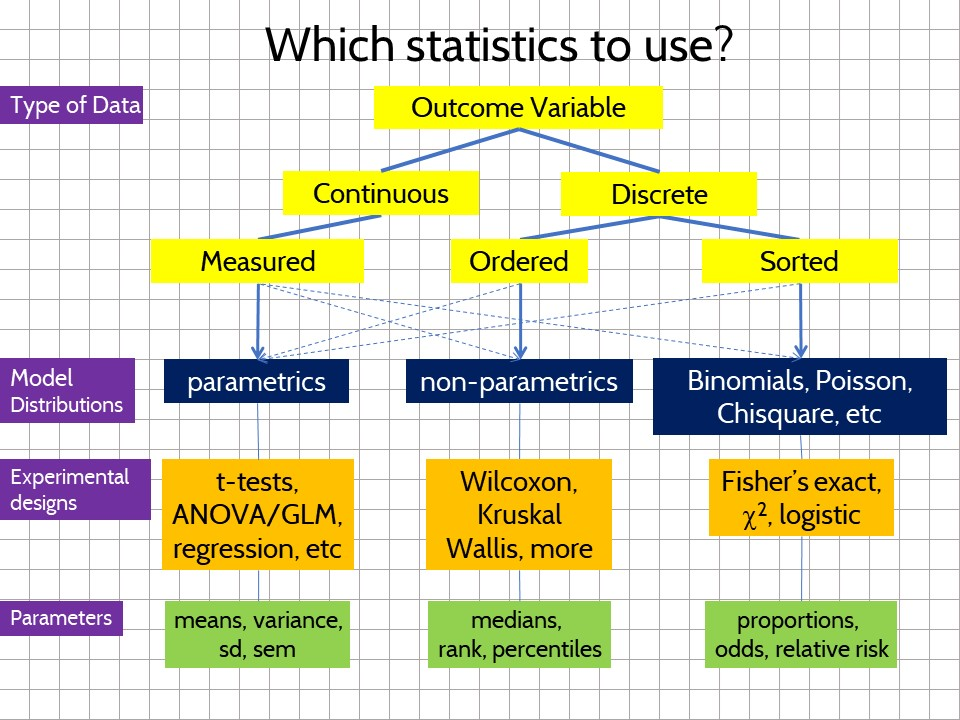
\includegraphics[width=13.33in]{images/testing_heuristic} \caption{The type of data dictates how it should be modeled.}\label{fig:unnamed-chunk-25}
\end{figure}

Third, the ``measured, ordered, sorted'' scheme classifies variables on the basis of their information density, where measured \textgreater{}\textgreater{} ordered \textgreater{}\textgreater{} sorted.

Different authors/softwares give these three types of variables different names, which creates some confusion. In SPSS, for example, when setting up variables you can choose to classify it as scalar, ordinal, or nominal, which correspond to measured, ordered and sorted. Another fairly common descriptive set for the three types is interval, ordinal, and categorical. These correspond to measured, ordered, and sorted, too.

Though they are named differently, for the most part everybody seems to agree that all variables can be reduced to 3 subtypes, even if they can't agree on what to name them.

\hypertarget{measured-variables}{%
\subsection{Measured variables}\label{measured-variables}}

Because everything is measured in some sense of the word ``measured''" is probably not an ideal choice to describe what is meant when refering to a continuous variable. My rationale for the choice is that it almost always requires some kind of measuring instrument to grab this type of data.

For the present purposes let's considered the terms measured variables and continuous variables as synonymous. Measured variables are fairly easy to spot. Any derivative of one of the \href{https://www.nist.gov/pml/weights-and-measures/metric-si/si-units}{seven base SI units} will be a measured variable.

\begin{Shaded}
\begin{Highlighting}[]
\NormalTok{knitr}\OperatorTok{::}\KeywordTok{include_graphics}\NormalTok{(}\StringTok{"images/si_units.jpg"}\NormalTok{)}
\end{Highlighting}
\end{Shaded}

\begin{figure}
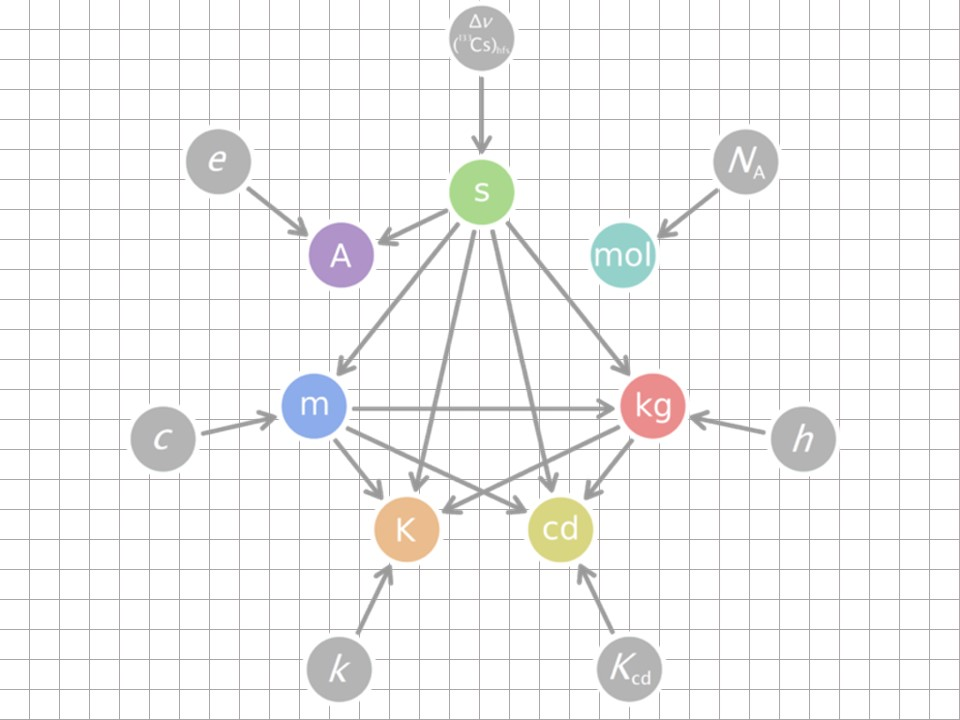
\includegraphics[width=13.33in]{images/si_units} \caption{The seven SI units}\label{fig:unnamed-chunk-26}
\end{figure}

Take mass as an example. The masses of physical objects can be measured on a continuous scale of sizes ranging from super-galaxian to subatomic. Variables that are in units of mass take on a smooth continuum of values over this entire range because mass scales are infinitesimily divisible.

Here's a thought experiment for what infinitesimily divisible means. Take an object that weighs a kilogram, cut it in half and measure what's left. You have two objects that are each one half a kilogram. Now repeat that process again and again. After each split something always remains whose mass can be measured. Even though it gets smaller and smaller. Even when you arrive at the point where only a single atom remains it can be smashed into yet even smaller pieces in a supercollider, yielding trails of subatomic particles\ldots{}.most of which have observable masses.

But here's what's important about continuous variables: That continuity between gradations means that continuous variables can carry more information than other types of variables. That's what I meant by information density, in the comment above.

On a scale of micrograms, an object weighing one kilogram would have one billion subdivisions. If you have an instrument that can accurately weigh the mass of kilogram-sized objects to the microgram level, and each microgam would be informative, you would say that one kilogram is comprised of a billion bits of information.

All of that possible information explains why the distinction between continuous and discrete variables is so important. You'll see that discrete variables lack this kind of information density between their units. As you read on below as discrete variables are discussed, think about how continuous variables carry more information than discrete variables.

More pragmatically, this difference is the basis for why discrete and continuous data behave so differently. And because of this inherent basis for why they behave differently, statisticians have devised statistical models that are more appropriate for one kind of data vs some other.

\hypertarget{discrete-categorical-and-ordinal-variables}{%
\subsection{Discrete categorical and ordinal variables}\label{discrete-categorical-and-ordinal-variables}}

Discrete variables are discontinuous. The units of discrete variables are indivisible. Unlike continuous variables, discrete variables offer no information between their unit scale boundaries.

There are two types of discrete variables. These are called \textbf{ordinal} and \textbf{categorical}. I like to call these ordered and sorted, respectively, again for alliterative purposes.

\hypertarget{sorted-data}{%
\subsubsection{Sorted data}\label{sorted-data}}

Categorical variables are a bit easier to understand so let's start with those. These variables represent objects that are counted. Because they have certain features they are sorted into categories or, as I like to say, buckets.

For example, a biostats class might be comprised of 50 students, 15 of whom are men and the rest are women. The name of the variable is \texttt{sex}. The values that the ``sex'' variable can take on is either \texttt{male} or \texttt{female}. The variable \texttt{sex} is a factoral variable at two levels.

If we count all of the men and woman in a class we arrive at another variable called \texttt{count} which represents the discrete counts of people who are sorted into either of the two sex categories.

The variable \texttt{count} is an integer varible. It cannot take on any values other than integer values. There cannot be a case that has less than a whole student. A partial biostats student would be absurd!

So our data set has two variables. One is \texttt{sex}, a factoral variable that has two levels. The other is \texttt{count}, an integer variable that has \$\le\$50 levels.

Of course, the categorization of sex is sometimes ambiguous. If it is important to accomodate more, we would add additional categories to account for all possible outcomes. For example, the \texttt{sex} variable could be set to take on values of \texttt{man}, \texttt{woman}, and \texttt{other}.

Take a moment to also think about the values of that \texttt{sex} variable. This is to emphasize that \texttt{man}, \texttt{woman} and \texttt{other} are not numeric values. Variables can have non-numeric values. R reads those levels as character values and ``coerces'' to classify \texttt{sex} as a factoral variable with three levels, \texttt{man}, \texttt{woman} and \texttt{other}.

Let's use R to create a summary table for the composition by sex of the biostats class. Inspection of the code shows the table has two variables, \texttt{sex} as described, and \texttt{count}. The function \texttt{str(ibs538)} reveals that the former variable is a ``Factor w/ 3 levels''" and the later is a integer variable. We used the \texttt{is.integer} function in the code to ensure that \texttt{count} would be an integer variable. Had we not, R wanted to coerce it as a numeric variable.

Finally, notice how the variable \texttt{count} is only comprised of discrete integer values. These discrete counts are why sorted data is classified as discrete.

\begin{Shaded}
\begin{Highlighting}[]
\NormalTok{sex <-}\StringTok{ }\KeywordTok{c}\NormalTok{(}\StringTok{"man"}\NormalTok{, }\StringTok{"woman"}\NormalTok{, }\StringTok{"other"}\NormalTok{)}
\NormalTok{count <-}\StringTok{ }\KeywordTok{as.integer}\NormalTok{(}\KeywordTok{c}\NormalTok{(}\DecValTok{15}\NormalTok{, }\DecValTok{35}\NormalTok{, }\DecValTok{0}\NormalTok{))}
\NormalTok{ibs538 <-}\StringTok{ }\KeywordTok{data.frame}\NormalTok{(sex, count); ibs538}
\end{Highlighting}
\end{Shaded}

\begin{verbatim}
##     sex count
## 1   man    15
## 2 woman    35
## 3 other     0
\end{verbatim}

\begin{Shaded}
\begin{Highlighting}[]
\KeywordTok{str}\NormalTok{(ibs538)}
\end{Highlighting}
\end{Shaded}

\begin{verbatim}
## 'data.frame':    3 obs. of  2 variables:
##  $ sex  : Factor w/ 3 levels "man","other",..: 1 3 2
##  $ count: int  15 35 0
\end{verbatim}

Obviously, there's nothing experimental about counting the sex of biostats students. However, many biomedical experiments generate discrete categorical data, too. Imagine the following:

\begin{itemize}
\tightlist
\item
  Neurons are poked with an electrode. Counts are recorded of the number of times they depolarize over a certain time period, in response to an depolarizing agent and its control.
\item
  Cells are stained for expression of a marker protein. The number of cells in which the protein is detected are counted. Counts of a knockdown condition are compared to a control.
\item
  By some criteria, cells are judged to be either alive or dead and counted as such. The number of alive cells are counted after manipulating expression of a tumor suppressor gene, and compared to a control.
\item
  By some criteria, mice are judged to either show a disease phenotype or not, and counted as such. Disease incidence is counted in response to levels of a therapeutic agent, or a background genotype, or in response to some stressor.
\end{itemize}

There are an infinite number of examples for experiments that can be performed in which a dependent variable is categorized and each of the replicates are sorted into one or some other level of that category. In the end, sometimes even after some fairly sophisticated instrumentation or biochemical analysis, all the researcher does is count objects that have a characteristic or some other.

Unlike continuous variables, discrete variables don't possess any information between their units. In each of the cases above the replicate either possesses a level of the variable or it does not. It belongs in one bucket or some other.

\hypertarget{ordered-data}{%
\subsubsection{Ordered data}\label{ordered-data}}

Ordered data is, in one sense, a hybrid cross of sorted and measured data.

If you've ever taken a poll in which you've been asked to evaluate something on a scale ranging from something akin to ``don't like at all'' to ``couldn't live without''\ldots{}then you've experienced ordinal scaling (such scales are called Likert scales). The precourse survey for this course is chock full of questions that generate data on an ordered scale.

Ordered variables are structured to have levels which are quantitatively related to each other.

Each experimental replicate is evaluated and then categorized to one of the values of the ordinal variable. It is true there is an element of sorting, but the key difference is these aren't nominal categories as in sorted data. There are underlying gradations of the variable's scale. This is not just the absence or presence of an attribute, but rather some amount of the attribute relative to other possible amounts the scale allows for.

These gradations within the levels of the ordered variable make them somewhat like measured data. The data strucure has intervals. But ordinal data are discrete because only certain values for the measurement are allowed, depending upon the structure of the scale or scoring system for a given attribute. There is no information between the intervals.

Disability status scales represent classic ordinal scales. These are used to assess neurologic abnormalities, for example, those associated with experimental multiple sclerosis. Each replicate in a study is evaluated by trained researchers and assigned the most appropriate value given its condition: 0 for no disease, 1 for limp tail, 2 for mild paraparesis, 3 for moderate paraparesis, 4 for complete hindlimb paralysis, and 5 for moribound.

Obviously, in this ordinal scale, as the numeric value increases so to does the severity of the subject's condition.

Here's what a very small set of ordinal data might look like:

\begin{Shaded}
\begin{Highlighting}[]
\NormalTok{genotype <-}\StringTok{ }\KeywordTok{c}\NormalTok{(}\KeywordTok{rep}\NormalTok{(}\StringTok{"wt"}\NormalTok{, }\DecValTok{3}\NormalTok{), }\KeywordTok{rep}\NormalTok{(}\StringTok{"ND4"}\NormalTok{, }\DecValTok{3}\NormalTok{))}
\NormalTok{DSS_score <-}\StringTok{ }\KeywordTok{as.integer}\NormalTok{(}\KeywordTok{c}\NormalTok{(}\DecValTok{0}\NormalTok{,}\DecValTok{1}\NormalTok{,}\DecValTok{1}\NormalTok{,}\DecValTok{5}\NormalTok{,}\DecValTok{3}\NormalTok{,}\DecValTok{5}\NormalTok{))}
\NormalTok{results <-}\StringTok{ }\KeywordTok{data.frame}\NormalTok{(genotype, DSS_score); results}
\end{Highlighting}
\end{Shaded}

\begin{verbatim}
##   genotype DSS_score
## 1       wt         0
## 2       wt         1
## 3       wt         1
## 4      ND4         5
## 5      ND4         3
## 6      ND4         5
\end{verbatim}

\begin{Shaded}
\begin{Highlighting}[]
\KeywordTok{str}\NormalTok{(results)}
\end{Highlighting}
\end{Shaded}

\begin{verbatim}
## 'data.frame':    6 obs. of  2 variables:
##  $ genotype : Factor w/ 2 levels "ND4","wt": 2 2 2 1 1 1
##  $ DSS_score: int  0 1 1 5 3 5
\end{verbatim}

\texttt{genotype} is an indepedent, factoral variable that comes in two levels, \texttt{wt} or \texttt{ND4}. \texttt{DSS\_score} is a dependent variable that comes in 6 levels, the integer values ranging from 0 to 5. We need to force R to read \texttt{DSS\_score} for what it is, an integer rather than as a numeric.

One of the key issues of ordinal scales is that they are not necessarily guassian. As a general rule they tend to be skewed (though there is no inherent reason for this to be the case).

For example, in my precourse survey I ask students how excited they are, on a scale of 1 to 10, to take a biostats class. The result is decidedly mixed. There's a bit of a lean towards good enthusiasm, but a fairly pronounced unenthusiastic tail.

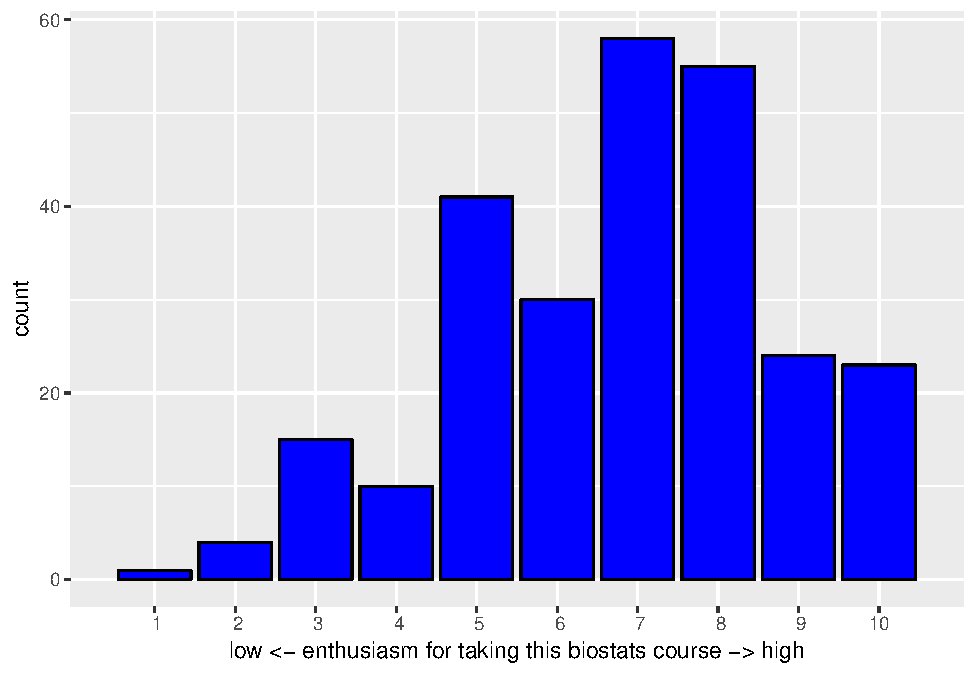
\includegraphics{jabstb_files/figure-latex/unnamed-chunk-29-1.pdf}

The data on this ordinal scale are not normally distributed. Any analysis would need to be with a statistical procedure that does not assume normally distributed dependent variables.

\begin{Shaded}
\begin{Highlighting}[]
\KeywordTok{ggplot}\NormalTok{(}\KeywordTok{data.frame}\NormalTok{(}\DataTypeTok{score =} \KeywordTok{c}\NormalTok{(}\DecValTok{1}\NormalTok{, }\DecValTok{25}\NormalTok{)), }
       \KeywordTok{aes}\NormalTok{(score)) }\OperatorTok{+}
\StringTok{  }\KeywordTok{stat_function}\NormalTok{(}\DataTypeTok{fun =}\NormalTok{ dnorm, }\DataTypeTok{args=}\KeywordTok{list}\NormalTok{(}\DataTypeTok{mean=}\DecValTok{15}\NormalTok{, }\DataTypeTok{sd=}\FloatTok{1.5}\NormalTok{)) }
\end{Highlighting}
\end{Shaded}

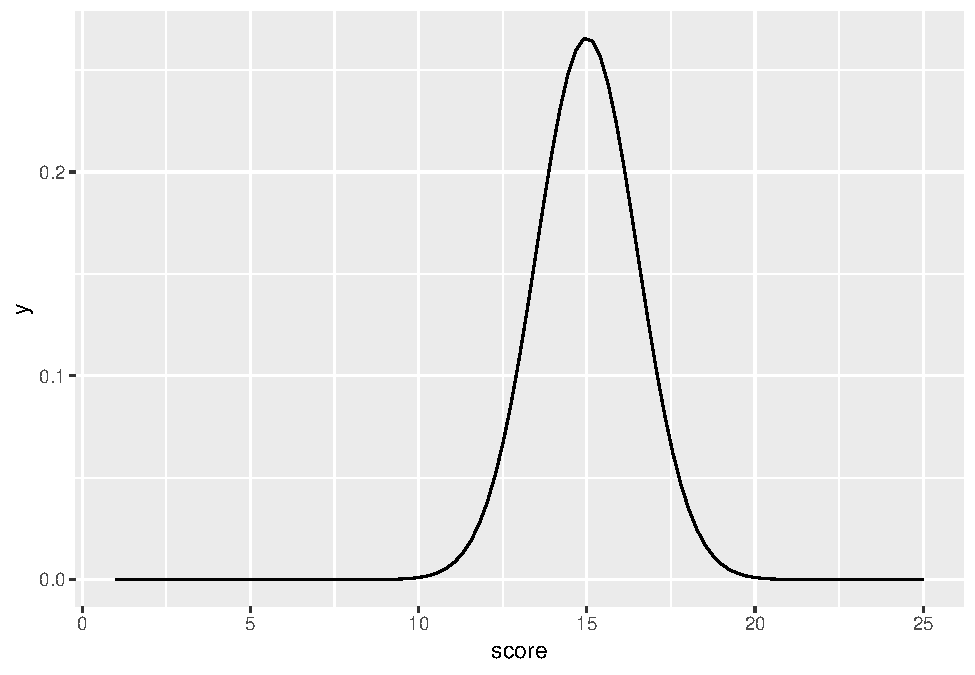
\includegraphics{jabstb_files/figure-latex/unnamed-chunk-30-1.pdf}

\begin{Shaded}
\begin{Highlighting}[]
\NormalTok{df <-}\StringTok{ }\KeywordTok{data.frame}\NormalTok{(}\DataTypeTok{score=}\KeywordTok{c}\NormalTok{(}\DecValTok{1}\OperatorTok{:}\DecValTok{25}\NormalTok{), }\DataTypeTok{y=}\KeywordTok{dpois}\NormalTok{(}\DecValTok{1}\OperatorTok{:}\DecValTok{25}\NormalTok{, }\DecValTok{15}\NormalTok{))}
\KeywordTok{ggplot}\NormalTok{(df, }\KeywordTok{aes}\NormalTok{(score, y))}\OperatorTok{+}
\StringTok{       }\KeywordTok{geom_col}\NormalTok{()}
\end{Highlighting}
\end{Shaded}

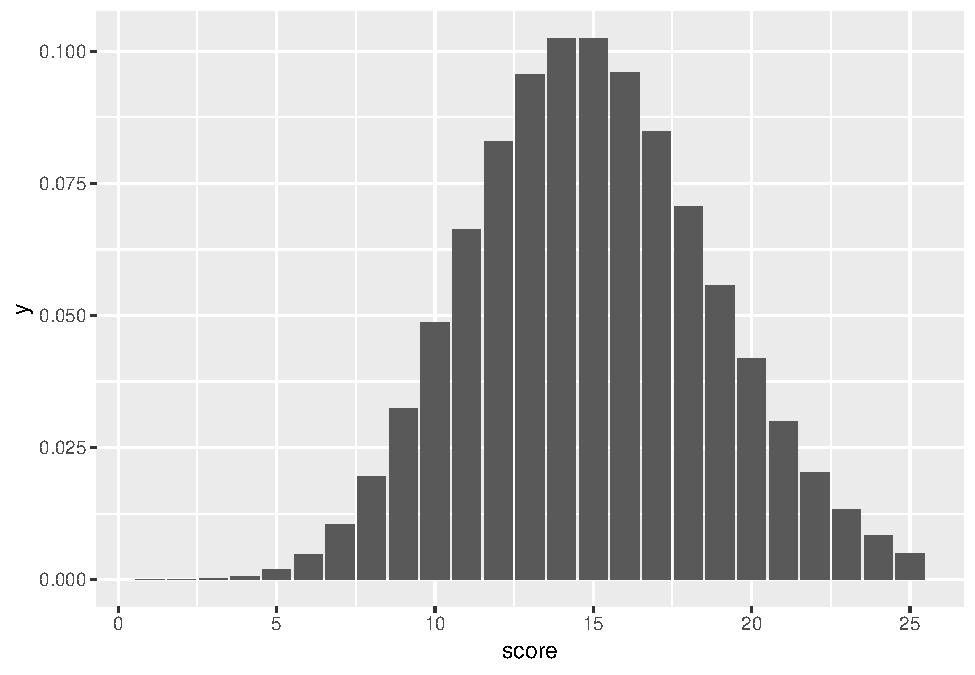
\includegraphics{jabstb_files/figure-latex/unnamed-chunk-30-2.pdf}

\begin{Shaded}
\begin{Highlighting}[]
\NormalTok{df <-}\StringTok{ }\KeywordTok{data.frame}\NormalTok{(}\DataTypeTok{score=}\KeywordTok{c}\NormalTok{(}\DecValTok{1}\OperatorTok{:}\DecValTok{25}\NormalTok{), }\DataTypeTok{y=}\KeywordTok{dbinom}\NormalTok{(}\DecValTok{1}\OperatorTok{:}\DecValTok{25}\NormalTok{, }\DecValTok{25}\NormalTok{, }\FloatTok{0.6}\NormalTok{))}
\KeywordTok{ggplot}\NormalTok{(df, }\KeywordTok{aes}\NormalTok{(score, y))}\OperatorTok{+}
\StringTok{       }\KeywordTok{geom_col}\NormalTok{()}
\end{Highlighting}
\end{Shaded}

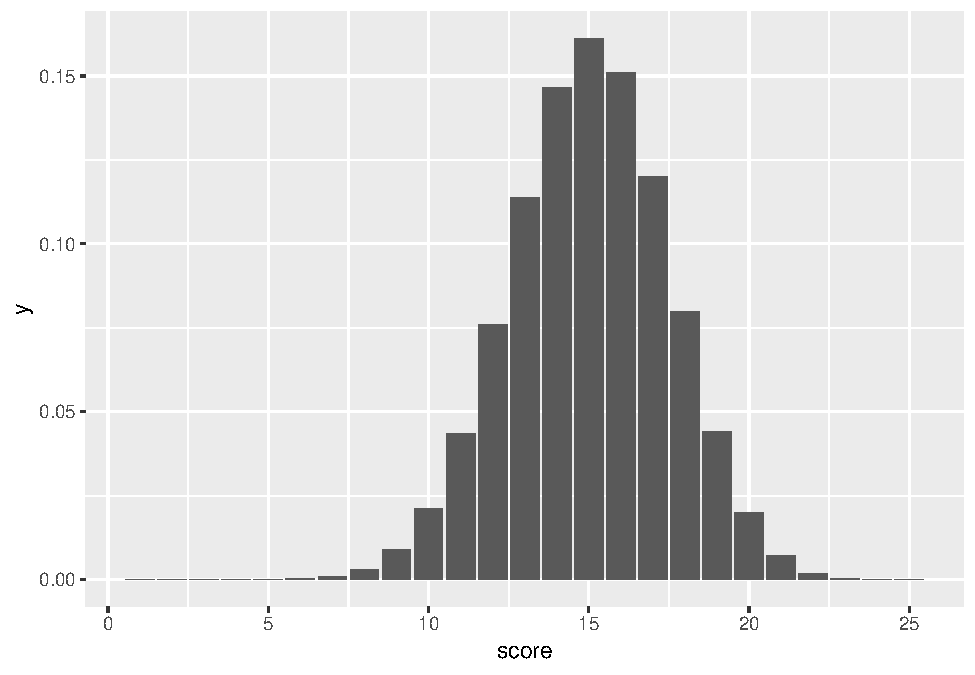
\includegraphics{jabstb_files/figure-latex/unnamed-chunk-30-3.pdf}

\hypertarget{statistics-for-categorical-data}{%
\chapter{Statistics for Categorical Data}\label{statistics-for-categorical-data}}

\begin{Shaded}
\begin{Highlighting}[]
\KeywordTok{library}\NormalTok{(PropCIs)}
\KeywordTok{library}\NormalTok{(tidyverse)}
\KeywordTok{library}\NormalTok{(binom)}
\KeywordTok{library}\NormalTok{(pwr)}
\KeywordTok{library}\NormalTok{(statmod)}
\KeywordTok{library}\NormalTok{(EMT)}
\end{Highlighting}
\end{Shaded}

Biomedical research is full of studies that count discrete events.

A common mistake made by many researchers is to use statistics designed for measured variables on discrete count variables. For example, they transform count data into scaler measures (eg, percents, folds etc) and then apply statistics designed for continuous variables to events that are fundamentally discrete by nature. The problem with that is there are inherent differences in the behaviors of continuous and discrete variables. Therefore, it is important to recognize

\hypertarget{types-of-categorical-data}{%
\section{Types of categorical data}\label{types-of-categorical-data}}

What proportion of cells express a specific antigen and does an experimental treatment cause that proportion to change? What proportion of rats treated with an anxiolytic drug choose one chamber over others in a maze test? How many people who express a certain marker go on to have cancer?

In these three scenarios the primary data are counts. All of the study results have integer values. The counts are categorized with variable attributes, thus they are called categorical data.

In fact, the three scenarios above are very different experimental designs. The first represent experiments that compare simple proportions. The second compare freqeuncies, and the third is an association study. The analysis of these require using a common suite of statistical tools in slightly different ways.

Broadly, all of these tools boil down to dealing with proportions. A few types of proportions (eg, odds ratio, relative risk) that can be calculated from these datasets are sometimes used as effect size parameters. Other times we'd use a confidence interval as a way of conveying an effect size. Statistical tests are then used to evaluate whether these effect sizes, or frequencies, or simple proportions, are extreme enough relative to null counterparts so that we can conclude the experimental variable had some sort of effect.

\hypertarget{proportions}{%
\subsection{Proportions}\label{proportions}}

We might\ldots{}

\begin{itemize}
\item
  Inactivate a gene hypothesized to function in the reproductive pathway. To test it, mating triangles would be set up to count the number of female mice that become pregnant or not.
\item
  Implant a tumor in mice, before counting the number of survivors and non-survivors at a given point later.
\item
  Mutate a protein that we hypothesize moves in and out of an intracellular compartment, before staining cells to count the number of cells where it is and is not located in a compartment of interest.
\end{itemize}

Each of the examples above have \texttt{binomial} outcomes\ldots{}pregnant vs not, dead vs alive, or inside vs outside.

In each case above, both the succesful and the failed events are counted in the experiment. A proportion is a simple ratio of counts of success to counts of failures.

\hypertarget{frequencies}{%
\subsection{Frequencies}\label{frequencies}}

Other kinds of counted data occur randomly in space and time. The examples below illustrate this. Note how only the number of events are recorded, rather than categorizing them as successes or failures. These counts therefore have the statistical property of frequency, such as counts per time or counts per volume or counts per area.

We can\ldots{}

\begin{itemize}
\item
  Expose a neuron to an excitatory neurotransmitter, then count the number of times it depolarizes over a given period of time.
\item
  In a model of asthma, count the number of immune cells that are washed out in a pulmonary lavage protocol after an immunosuppressive agent.
\end{itemize}

The key difference for these are that their non-event counterparts are meaningless. For example, it is not possible to measure the number of depolarizations that don't occur, or know the number of immune cells that don't wash out in the lavage.

\hypertarget{associations}{%
\subsection{Associations}\label{associations}}

Lastly, the examples below illustrate the design of association studies, which are based upon, according to the null hypothesis, independent predictors and outcomes.

Here are some examples of association study designs:

You might wish to

\begin{itemize}
\item
  identify causal alleles associated with a specific disease phenotype by counting the number of people with and without the disease, who have or don't have a particular allelic variants.
\item
  determine if a history of exposure to certain carcinogens is associated with a higher risk of cancer by counting people with cancer who have been exposed.
\item
  know if a drug treatment causes a higher than expected frequency of a side-effect by counting the people on the drug with the side-effect.
\end{itemize}

In the simplest (and most general) case, association studies are 2X2 in design: A predictor is either present or absent as the row factor, and an outcome was either a success for a failure as the column factor. Subjects are categorized into groups on the basis of where they fall in the 4 possible combinations that such 2X2's allow for.

It should be noted that higher order association studies are also possible, which can be either symmetric (eg, 3x3) or non-symmetric (eg,) 9X2, 2x3, and so on.

\hypertarget{statistics-covered-here}{%
\subsection{Statistics Covered Here}\label{statistics-covered-here}}

\begin{itemize}
\tightlist
\item
  Confidence intervals of proportions
\item
  One-sample proportions test
\item
  Two-sample proportions test
\item
  Goodness of fit tests
\item
  Tests of associations
\item
  Power analysis of proportions (including Monte Carlo simulation)
\item
  Plotting proportions with ggplot2
\end{itemize}

\hypertarget{exact-v-asymptotic-calculations-of-p-values}{%
\section{Exact v Asymptotic Calculations of p-values}\label{exact-v-asymptotic-calculations-of-p-values}}

The statistical tests for hypotheses on categorical data fall into two broad categories: exact tests (\texttt{binom.test}, \texttt{fisher.test}, \texttt{multinomial.test}) and asymptotic tests (\texttt{prop.test} \texttt{chisq.test}).

Exact tests calculate exact p-values. That's made possible using factorial math. The \texttt{prop.test} and \texttt{chisq.test} generate asymptotic (aka, approximate) p-values. They calculate a \(\chi^2\) test statistic from the data before mapping it to a \(\chi^2\) probability density function. Because that function is continuous, the p-values it generates are asymptotically-estimated, rather than exactly calculated.

\hypertarget{choosing-exact-or-asymptotic}{%
\subsection{Choosing exact or asymptotic}\label{choosing-exact-or-asymptotic}}

As a general rule, given the same datasets and arguments, exact and approximate hypothesis test functions will almost always give you p-values that differ, but only slightly.

That's usually not a problem unless you're near a threshold value. Typically, an integrity crisis is evoked when that happens: ``Which is''right???" Do you p-hack and choose the favorable one or not?

You should use the test you said you'd use when you first designed the experiment. And if you didn't pre-plan\ldots{}or at least have some idea about where you are going\ldots{}recognize that the exact tests are more accurate.

Another issue that arises is how well the tests perform with low count numbers. For example, as a rule of thumb, avoid using the \texttt{chisq.test} when the data have counts less than 5 in more than 20\% of the cells because the accuracy of the \texttt{chisq.test} is less at low cell counts. Use an exact test instead.

\hypertarget{overview-of-the-types-of-hypothesis-testing}{%
\section{Overview of the types of hypothesis testing}\label{overview-of-the-types-of-hypothesis-testing}}

We'll go through each below in more detail, emphasizing practical experimental design and interpretation principles.

\hypertarget{proportion-analysis}{%
\subsection{Proportion analysis}\label{proportion-analysis}}

You can learn a lot about experimental statistics by thinking about proportions. So a lot of time is spent on it. Proportions are derived from events that can be classified as either successes or failures. Sometimes we want to compare simple proportions to decide if they are the same or not.

\hypertarget{goodness-of-fit-testing}{%
\subsection{Goodness of fit testing}\label{goodness-of-fit-testing}}

We do this when we want to compare the frequency distribution we observe in an experiment to the null expectation for that frequency distribution.

\hypertarget{contingency-analysis}{%
\subsection{Contingency Analysis}\label{contingency-analysis}}

Contingency analysis, otherwise known as tests of independence, are very different from goodness-of-fit test and simple proportion tests, in design and in purpose. They allow us to ask if two (or more) variables are associated with each other. Unlike a lot of the statistics we'll deal with, there is a hint of a predictive element associated with these types of studies because the effect sizes we use to explain their results are related to odds and risk and likelihood. Which is not to say that we couldn't use the same predictive concepts in proportions and goodness of fit testing.

Contingency tests are very common in epidemiology and in clinical science. You recognize by their names as cohort studies, case control studies, and so forth.

\hypertarget{comparing-proportions}{%
\section{Comparing proportions}\label{comparing-proportions}}

In their simplest use, the tests here can be used to compare one proportion to another. Is the proportion of successes to failures that results from a treatment different from the proportion that results from control? We'll dive into this further below.

\hypertarget{a-mouse-t-cell-pilot-experiment-the-cytokine-inducible-antigen-gradstudin}{%
\subsection{A Mouse T Cell Pilot Experiment: The Cytokine-inducible antigen gradstudin}\label{a-mouse-t-cell-pilot-experiment-the-cytokine-inducible-antigen-gradstudin}}

Let's imagine a small pilot experiment to see how a cytokine affects T cells. This is a very crude experiment designed mostly to illustrate some principles.

A cytokine is injected into a single mouse. There is no control injection, just one mouse/one cytokine injection. A time later, blood is harvested from the mouse to measure an antigen on T cells. Let's call the antigen gradstudin.

Assume a method exists to detect T cells in the sample that express gradstudin and don't express gradstudin.

That method implies some \texttt{nominal} criteria are established to \texttt{categorize} T cells as either expressing gradstudin or not. FACS machines are very useful for this. The machine typically produces \texttt{continuous} fluorescent data, where intensity is proportional to gradstudin levels. But we don't care about the magnitude of the expression level, we just care whether it is there or not.

Based upon our scientific expertise, we establish cutoff gating criteria above which fluoresence == gradstudin is present.

The machine therefore returns simple counts of both gradstudin-positive and gradstudin-negative cells.

\hypertarget{calculating-proportions}{%
\subsection{Calculating Proportions}\label{calculating-proportions}}

Here's the data, counts of cells expressing and not expressing gradstudin. It is a very simple dataset:

\begin{Shaded}
\begin{Highlighting}[]
\NormalTok{pos <-}\StringTok{ }\DecValTok{5042}
\NormalTok{neg <-}\StringTok{ }\DecValTok{18492}
\end{Highlighting}
\end{Shaded}

\textbf{A proportion is the count of a particular outcome relative to the total number of events.} It's customary to use the number of successes as the numerator. Whereas its customary to refer to the total number of events, \texttt{n}, as the trial number rather than as sample size, but they mean the same thing.

\begin{Shaded}
\begin{Highlighting}[]
\NormalTok{n <-}\StringTok{ }\NormalTok{pos}\OperatorTok{+}\NormalTok{neg }\CommentTok{#trial size}
\NormalTok{prop <-}\StringTok{ }\NormalTok{pos}\OperatorTok{/}\NormalTok{n}
\NormalTok{prop}
\end{Highlighting}
\end{Shaded}

\begin{verbatim}
## [1] 0.2142432
\end{verbatim}

\hypertarget{what-a-proportion-estimates}{%
\subsection{What A Proportion Estimates}\label{what-a-proportion-estimates}}

This sample proportion is descriptive statistic. It serves as a \texttt{point\ estimate} of the true proportion of the population we sampled. The only way to know the true proportion would be to count every T cell in every drop of the subjects blood!

This point estimate is statistically valid if our sample meets two conditions. First, that this is a random sample of the T cells in the subject's blood. Second, if we consider every T cell in the sample as statistically independent of every other T cell.

We can safely assume those conditions are met. Strictly, as an estimate this proportion only infers the population of blood borne T cells in that one subject. We really can't generalize much further than that, including the composition of T cells in sequesterd compartments (thymus, nodes, etc).

Which is fine for our purposes now because we're trying to keep this simple.

\hypertarget{confidence-intervals-of-proportions}{%
\subsection{Confidence Intervals of Proportions}\label{confidence-intervals-of-proportions}}

Confidence intervals (CI) have features of both descriptive and inferential statistics.

\hypertarget{definition-of-a-95-ci}{%
\subsubsection{Definition of a 95\% CI}\label{definition-of-a-95-ci}}

\textbf{The 95\% CI for a sample proportion represents a range of proportions within which 95\% of the time we would expect the true population proportion.}

There's a lot going on there.

The value of the proportion we measured in the sample is a mathematical fact that is not in dispute. It is what it is. The question is, what does it represent?

Although there might be some error associated with measuring it, our single sample offers no real information about what that error might be. As an n=1 sample, there is no variation!

\textbf{What is unknown is the true proportion of gradstudin+ T cells in the population we sampled.}

CI's are designed to give us some insights into that unknown.

95\% CI's are a \texttt{range\ estimate} of what that true population proportion might be. CI's are calculated in part upon the quality of the point estimate. In the case of proportions, the quality of the point estimate is driven by the size of the sample, the number of counts that are involved in calculating the proportion.

As you might imagine intuitively, the more counts we have in the sample, the more confidence we should have that our proportion provides a good estimate of the population's proportion.

\hypertarget{calculating-ci-with-r}{%
\subsubsection{Calculating CI with R}\label{calculating-ci-with-r}}

The \texttt{PropCIs} package offers several ways to calculate a CI. Is one better than the other? Sometimes, yes. For now, let's not worry about that. \href{http://www.ucl.ac.uk/english-usage/staff/sean/resources/binomialpoisson.pdf}{Wilson's score interval with continuity correction}{]} is suggested as the most accurate for proportions.

When publishing it is important is to state which CI method is used. Other methods are more commonly used than Wilson's because they gained traction as being easier to compute by hand, and old habits die slowly.

Taking the data on cytokine induced gradstudin+ T cells, the chunk below illustrates how to use \texttt{PropCIs} to derive a Wilscon score interval-based 95\% CI:

\begin{Shaded}
\begin{Highlighting}[]
\KeywordTok{scoreci}\NormalTok{(pos, n, }\DataTypeTok{conf.level=}\FloatTok{0.95}\NormalTok{)}
\end{Highlighting}
\end{Shaded}

\begin{verbatim}
## 
## 
## 
## data:  
## 
## 95 percent confidence interval:
##  0.2090 0.2195
\end{verbatim}

\hypertarget{interpretation-of-a-ci}{%
\subsubsection{Interpretation of a CI}\label{interpretation-of-a-ci}}

The value of our sample proportion, 0.214, falls within this 95\% CI. That's not a big surprise, given the 95\% CI was calculated from our proportion!

On the basis of the sample proportion, we can conclude from this CI that there is a 95\% chance the true proportion of gradstudin positive T cells falls within this very narrow range.

\hypertarget{using-the-ci-as-a-quick-test-of-statistical-significance.}{%
\subsubsection{Using the CI as a quick test of statistical significance.}\label{using-the-ci-as-a-quick-test-of-statistical-significance.}}

Let's say, for example, that we have tremendous experience and great scientific reason to expect to see under normal conditions that only 15\% of T cells would be gradstudin-positive normally. Does our sample proportion differ from that expectation?

Since a proportion of 0.15 is not within the 95\% CI calculated above, we can conclude that the cytokine-induced sample proportion differs from this expectation at the 5\% level of statistical significance.

We just did a statistical test, without running any software (sorta) or generating any p-values!! And it is perfectly valid inference.

\hypertarget{a-one-sample-proportion-test}{%
\subsection{A One-Sample Proportion Test}\label{a-one-sample-proportion-test}}

We'll use \texttt{prop.test} to run a test that generates a p-value to decide if the sample proportion we have above differs from 0.15.

\hypertarget{hypothesis-tested-in-a-one-sample-proportion-test}{%
\subsubsection{Hypothesis Tested in a One-Sample Proportion Test}\label{hypothesis-tested-in-a-one-sample-proportion-test}}

In this test the sample antigen-positive proportion is compared to a theoretical proportion. If the typical proportion of antigen-positive T cells within a blood sample is 15\%, is the result after cytokine treatment different from this proportion?

Let's say that our scientific hypothesis going into all this is that the cytokine induces the antigen on T cells. Since we are predicting an increase, we should establish a one-sided alternative (thus using \texttt{greater} as an argument in \texttt{prop.test} below) as our statistical hypothesis.

Our statistical hypothesis is the null. We'll decide whether or not to reject the null on the basis of the test results. Philosophically, we're using a falsification method.

\begin{itemize}
\item
  The statistical alternate hypothesis: \(\pi>15\%\)
\item
  The statistical null hypothesis: \(\pi\le15\%\)
\end{itemize}

We use Greek notation to represent the `true' population proportion. This reminds us that a statistical hypothesis is an inferential test about the population proportion.

Again, there is no question that the sample proportion differs from a proportion of 15\%. 21\% != 15\%. That's a simple numerical fact. Statistical tests are not necessary to make that assertion.

On the basis of the sample proportion p, we'd like to draw inference on the composition of all of the T cells in the blood of the subject. Thus, the sample p is only an estimate of a true \(\pi\) (which we notate using Greek letters).

Statistical testing allows us to generate some insight into the reliability of our estimate.

The chunk below lays out these arguments using R's \texttt{prop.test} function:

\begin{Shaded}
\begin{Highlighting}[]
\CommentTok{#pos and n in the test arguments are objects that were defined above!}
\KeywordTok{prop.test}\NormalTok{(}
\NormalTok{  pos, n, }\DataTypeTok{p=}\FloatTok{0.15}\NormalTok{, }
  \DataTypeTok{alternative =} \StringTok{"greater"}\NormalTok{, }
  \DataTypeTok{conf.level =} \FloatTok{0.95}\NormalTok{, }
  \DataTypeTok{correct =} \OtherTok{TRUE}
\NormalTok{  )}
\end{Highlighting}
\end{Shaded}

\begin{verbatim}
## 
##  1-sample proportions test with continuity correction
## 
## data:  pos out of n, null probability 0.15
## X-squared = 761.29, df = 1, p-value < 2.2e-16
## alternative hypothesis: true p is greater than 0.15
## 95 percent confidence interval:
##  0.2098559 1.0000000
## sample estimates:
##         p 
## 0.2142432
\end{verbatim}

\hypertarget{interpreting-one-sample-prop.test-output}{%
\subsubsection{Interpreting one-sample prop.test output}\label{interpreting-one-sample-prop.test-output}}

Like all statistical tests, this one is evaluated under the assumption that the null hypothesis is true. We use the test outcome to decide whether the null hypothesis should be rejected.

The \texttt{prop.test} conducts a chi-square analysis. The value of \(\chi^2\) for this sample is very large.

\textbf{The p-value represents the probability of obtaining a \(\chi^2\) value as larger or larger then what is calculated from our sample.}

If the null hypothesis is true in this case, the probability of a \(\chi^2\) value as large or larger than we obtained is 2.2e-16, which is very, very low.

The 95\% CI is 0.2098 to 1.0. There is a 95\% chance the population proportion is greater than 0.2098. The reason it differs from the Wilson's CI calculated above is that we used \texttt{greater}as a one-sided hypothesis argument in the prop.test.

\hypertarget{how-to-write-this-up}{%
\subsubsection{How to write this up}\label{how-to-write-this-up}}

\emph{The proportion of gradstudin positive T cells after cytokine treatment in the subject differs from an expected value of 0.15 (one-sided one-sample proportions test, p-value=2.2e-16, 95\% CI = 0.209 to 1.0)}

Notice how I didn't say ``significantly'' or ``statistically significantly'' or some such. Whether an outcome is signficant or not should be a scientific assertion, rather than statistical.

\hypertarget{an-exact-test-for-one-proportion}{%
\subsubsection{An exact test for one proportion}\label{an-exact-test-for-one-proportion}}

R's \texttt{binom.test} function is an exact test for whether a proportion differs from a theoretical expectation. It compares proportions using an entirely different procedure.

As a \textbf{one-proportion test} the \texttt{binom.test} gives an exact p-value derived from the binomial distribution, whereas the \texttt{prop.test} gives approximate p-values because it uses the chi-square distribution.

That distinction is hard to see with our examples here, but the differences will become more noticable when analyzing samples with far fewer events.

Here's the binomial test run on two different proportions. In each, the test is comparing the experimental proportion to the proportion value of 0.15.

\begin{Shaded}
\begin{Highlighting}[]
\KeywordTok{binom.test}\NormalTok{(pos, n, }\DataTypeTok{p=}\FloatTok{0.15}\NormalTok{)}
\end{Highlighting}
\end{Shaded}

\begin{verbatim}
## 
##  Exact binomial test
## 
## data:  pos and n
## number of successes = 5042, number of trials = 23534, p-value <
## 2.2e-16
## alternative hypothesis: true probability of success is not equal to 0.15
## 95 percent confidence interval:
##  0.2090155 0.2195416
## sample estimates:
## probability of success 
##              0.2142432
\end{verbatim}

\begin{Shaded}
\begin{Highlighting}[]
\KeywordTok{binom.test}\NormalTok{(}\DataTypeTok{x=}\DecValTok{567}\NormalTok{, }\DataTypeTok{n=}\DecValTok{1778}\NormalTok{, }\DataTypeTok{p=}\FloatTok{0.15}\NormalTok{)}
\end{Highlighting}
\end{Shaded}

\begin{verbatim}
## 
##  Exact binomial test
## 
## data:  567 and 1778
## number of successes = 567, number of trials = 1778, p-value <
## 2.2e-16
## alternative hypothesis: true probability of success is not equal to 0.15
## 95 percent confidence interval:
##  0.2972673 0.3411272
## sample estimates:
## probability of success 
##              0.3188976
\end{verbatim}

\hypertarget{comparing-two-proportions}{%
\subsection{Comparing Two Proportions}\label{comparing-two-proportions}}

We can stick with the T cell-cytokine-gradstudin scenario, but let's change up the experiment a tad.

Let's imagine we've withdrawn a sample of blood from a subject and enriched for T cells. Half of the sample is exposed in vitro to a cytokine for a few hours. The other half is exposed to vehicle as a control. We count the gradstudin-positive and gradstudin-negative T cells in both groups.

We now have a predictor group at two levels (treatment = vehicle or cytokine) and an outcome group at two levels (antigen = positive or negative)

\hypertarget{hypothesis-tested}{%
\subsubsection{Hypothesis Tested}\label{hypothesis-tested}}

Let's test the hypothesis that the proportion of postive T cells in the two samples differ. The choice is not to test whether one proportion is greater than the other. We just want to know if they differ.

The statistical hypotheses here differs from the one sample hypotheses in two ways.

First, notice how we're comparing the population proportion of cytokine- to that for vehicle-treatment.

Second, we're making this a two-tailed (\texttt{two.sided}) test instead of one-tailed (\texttt{greater}).

\begin{itemize}
\item
  The statistical alterate hypothesis: \(\pi_c\ne\pi_v\)
\item
  The statistical null hypothesis: \(\pi_c=\pi_v\)
\end{itemize}

A second way of writing these hypotheses to say the same thing:

\begin{itemize}
\item
  Alternate: \(\pi_c-\pi_v\ne0\)
\item
  Null: \(\pi_c-\pi_v=0\)
\end{itemize}

\hypertarget{running-the-test}{%
\subsubsection{Running the test}\label{running-the-test}}

Let's say that here are the outcome data:
gradstudin-positive, gradstudin-negative, total
Cytokine-treated: 567, 1211, 1778
Vehicle-treated: 412, 1485, 1897

The data can be dumped directly into \texttt{prop.test}. Normally we'd run this at 0.95 confidence level (type1 error of 5\%). Let's say we have good scientific reasons to run this test at a much more stringet threshold level for type1 error, because we're really hoping to avoid a false positive:

\begin{Shaded}
\begin{Highlighting}[]
\KeywordTok{prop.test}\NormalTok{(}
  \DataTypeTok{x=}\KeywordTok{c}\NormalTok{(}\DecValTok{567}\NormalTok{, }\DecValTok{412}\NormalTok{),}
  \DataTypeTok{n=}\KeywordTok{c}\NormalTok{(}\DecValTok{1778}\NormalTok{, }\DecValTok{1897}\NormalTok{),}
  \DataTypeTok{conf.level=}\FloatTok{0.9999999}
\NormalTok{  )}
\end{Highlighting}
\end{Shaded}

\begin{verbatim}
## 
##  2-sample test for equality of proportions with continuity
##  correction
## 
## data:  c(567, 412) out of c(1778, 1897)
## X-squared = 48.066, df = 1, p-value = 4.121e-12
## alternative hypothesis: two.sided
## 99.99999 percent confidence interval:
##  0.02364902 0.17977620
## sample estimates:
##    prop 1    prop 2 
## 0.3188976 0.2171850
\end{verbatim}

\hypertarget{interpretion-of-two-sample-proportions-test-output}{%
\subsubsection{Interpretion of Two-Sample proportions test output}\label{interpretion-of-two-sample-proportions-test-output}}

This test is evaluated under the assumption that the null hypothesis is true. The test results helps us decide whether the null hypothesis should be rejected. We'll do that if the p-value is less than our type1 error threshold.

The \texttt{prop.test} conducts a chi-square analysis using the Yates continuity correction. This \(\chi^2\) value is very large; extremely large.

The p-value represents the probability of obtaining a \(\chi^2\) value as larger or larger than that by chance. If the null hypothesis is true in this case, the probability of that sized \(\chi^2\) value is 4.12e-12, which is very low, and still much lower than our type1 error threshold.

We can reject the null.

If we subtract prop2 from prop1 we get a value of about 0.1017, as a point estimate for the difference between the two proportions.

The 99.99999\% CI for the difference between two proportions does not include the value of 0. Since the 99.99999\% CI does not overlap with 0, we can conclude from it alone that there is a difference between the two proportions. Even at this extremely high confidence level!!

\hypertarget{write-up}{%
\subsubsection{Write Up}\label{write-up}}

\emph{The proportion of gradstudin positive T cells after cytokine differs from that in vehicle treated cells (two-sided two-sample proportions test, p-value=4.12e-12, 99.99999\% CI for proportion difference = 0.023 to 0.179)}

Note how we don't say ``statistically significantly different''.

\hypertarget{exact-tests-for-two-proportions}{%
\section{Exact tests for two proportions}\label{exact-tests-for-two-proportions}}

An alternative to \texttt{prop.test} to \textbf{compare two proportions} is the \texttt{fisher.test}, which like the \texttt{binom.test} calculates exact p-values. The \texttt{fisher.test} requires that data be input as a matrix or table of the successes and failures.

We need to make a matrix of the data first, then perform the \texttt{fisher.test} on that matrix:
gradstudin-positive, gradstudin-negative, total
Cytokine-treated: 567, 1211, 1778
Vehicle-treated: 412, 1485, 1897

Notice below that here we're entering the successes and the failures in the matrix. We're tagging the matrix with some dimension names so it doesn't get confusing.

\begin{Shaded}
\begin{Highlighting}[]
\NormalTok{M <-}\StringTok{ }\KeywordTok{matrix}\NormalTok{(}
  \KeywordTok{c}\NormalTok{(}\DecValTok{567}\NormalTok{, }\DecValTok{412}\NormalTok{, }\DecValTok{1211}\NormalTok{, }\DecValTok{1485}\NormalTok{), }
  \DataTypeTok{nrow=}\DecValTok{2}\NormalTok{, }
  \DataTypeTok{dimnames =} \KeywordTok{list}\NormalTok{(}
    \DataTypeTok{Treat=}\KeywordTok{c}\NormalTok{(}\StringTok{"Cytokine"}\NormalTok{, }\StringTok{"Vehicle"}\NormalTok{), }
    \DataTypeTok{Antigen=}\KeywordTok{c}\NormalTok{(}\StringTok{"Positive"}\NormalTok{, }\StringTok{"Negative"}\NormalTok{)}
\NormalTok{    )}
\NormalTok{  )}
\NormalTok{M}
\end{Highlighting}
\end{Shaded}

\begin{verbatim}
##           Antigen
## Treat      Positive Negative
##   Cytokine      567     1211
##   Vehicle       412     1485
\end{verbatim}

\begin{Shaded}
\begin{Highlighting}[]
\KeywordTok{fisher.test}\NormalTok{(M)}
\end{Highlighting}
\end{Shaded}

\begin{verbatim}
## 
##  Fisher's Exact Test for Count Data
## 
## data:  M
## p-value = 3.433e-12
## alternative hypothesis: true odds ratio is not equal to 1
## 95 percent confidence interval:
##  1.451760 1.962188
## sample estimates:
## odds ratio 
##   1.687312
\end{verbatim}

Notice the output differs from the prop.test. In adddition to a p-value, the Fisher test produces an odds ratio and its confidence interval. The p-value leads to the same result and write-up as for the two proportion test. The odds ratio could be interpreted like this:

\emph{The cytokine increases the odds of gradstudin+ T cells by 1.687 compared to vehicle treatment (Fisher's Exact Tet for Count Data, p = 3.433e-12, OR 95\% CI = 1.45 to 1.96)}.

\hypertarget{goodness-of-fit-tests}{%
\section{Goodness of fit Tests}\label{goodness-of-fit-tests}}

Goodness-of-fit tests are useful for testing hypotheses about patterns of counts in time or space\ldots{}whether the distribution of their observed frequencies differs from expectations of a null case. In other words, do they occur in a non-random pattern?

There is no independent variable in these tests.

The shape of these datasets is either as 1 row or 1 column, where every cell is a time or space and the cell value is the the number of counts that occured in that time or space.

Either the \texttt{multinomial.test} (for exact p-values) or the \texttt{chisq.test} (for approximate p-values) can be used for Goodness-of-fit testing. The latter is most commonly used.

These designs compare the disribution of events to a hypothetical (or expected) model null distribution of those events.

These expected counts are entered in the test script as a \texttt{prop} or \texttt{p} argument. \emph{This can be confusing. It's important to recognize you should enter a vector of null probabilities in p or prop! Don't enter the counts you hope to see if the test were positive!!!}

Say we had a spatial memory test in which 28 independent subjects are placed into a maze for testing (one at a time) and we count which of 4 chambers they enter first. They do so at the following frequencies: A=14, B=3, C=7, D=4. Does this frequency distribution differ from the null expectation, A=7, B=7, C=7, D=7, where no chamber is more likely to be entered than another?

Failure is not an option in this design! Only successes are counted. Given enough time, a subject will always choose a chamber. If one fails the task, it must be censured. Let's test this at the 5\% type1 error threshold:

\hypertarget{an-exact-goodness-of-fit-test}{%
\subsection{An Exact Goodness of Fit test}\label{an-exact-goodness-of-fit-test}}

NB:The multinomial.test function requires you to assert the null frequency distribution explicitly and as fractions whose sum is 1.

\begin{Shaded}
\begin{Highlighting}[]
\NormalTok{x <-}\StringTok{ }\KeywordTok{c}\NormalTok{(}\DataTypeTok{A=}\DecValTok{14}\NormalTok{, }\DataTypeTok{B=}\DecValTok{3}\NormalTok{, }\DataTypeTok{C=}\DecValTok{7}\NormalTok{, }\DataTypeTok{D=}\DecValTok{4}\NormalTok{)}
\NormalTok{prob <-}\StringTok{ }\KeywordTok{c}\NormalTok{(}\DataTypeTok{A=}\NormalTok{.}\DecValTok{25}\NormalTok{, }\DataTypeTok{B=}\NormalTok{.}\DecValTok{25}\NormalTok{, }\DataTypeTok{C=}\NormalTok{.}\DecValTok{25}\NormalTok{, }\DataTypeTok{D=}\NormalTok{.}\DecValTok{25}\NormalTok{)}

\KeywordTok{multinomial.test}\NormalTok{(}
\NormalTok{  x, }
  \DataTypeTok{prob=}\NormalTok{prob}
\NormalTok{  )}
\end{Highlighting}
\end{Shaded}

\begin{verbatim}
## 
##  Exact Multinomial Test, distance measure: p
## 
##     Events    pObs    p.value
##       4495   1e-04     0.0235
\end{verbatim}

Note on the \texttt{multinomial.test}output: \href{http://rinterested.github.io/statistics/multinomial_exact.html}{Please see this site} for further information on what is represented by events (its a combination result--a metric of the computation it took to do this) and pObs (its a multinomial probability).

We're only intersted in the p-value, since we're using this function as an exact goodness-of-fit hypothesis test for the null hypothesis.

Why use an exact test rather than a \texttt{chisq.test}? Because we have two cells in the dataset with counts \textless{} 5! An exact p-value will be more accurate.

The test compares our sample frequency distribution to that in the null model. We actually wrote the latter explicitly in the function argument: null is uniform distribution--the subjects are equally likely to enter each chamber.

H0: The probability of choice is equal for each chamber.
\(\pi_A=\pi_B=\pi_C=\pi_D\)
H1: The probability of choice is not equal for each chamber.
\(\pi_A\ne\pi_B\ne\pi_C\ne\pi_D\)

(Note: this is an omnibus test. It doesn't explicity tell us which chambers are preferred by the subjects.)

Because the p-value is less than 0.05, we reject the null hypothesis and conclude that the chamber choice is not equitable across the four options.

\hypertarget{write-up-1}{%
\subsubsection{Write up}\label{write-up-1}}

\emph{In a 4 chamber maze test, the subjects displayed a clear, non-uniform chamber preference (Exact Multinomial Test, n=28, p=0.0235)} Note how this implies the null hypothesis.

\hypertarget{an-approximate-goodness-of-fit-test}{%
\subsection{An Approximate Goodness of Fit test}\label{an-approximate-goodness-of-fit-test}}

The \(\chi^2\) test of the same data is really simple to execute. It offers the same conclusion, but note how the p-value is very different.

Note also that we didn't enter the null frequency argument. The \texttt{chisq.test}function will coerce the null distribution if it is not entered as an argument explicitly, as you can see from the output for the second line. If for some reason to test against a non-uniform null distribution, you'll need to write that in your argument explicitly (eg, p = c(A=0.5, B=0.25, C \& D = 0.125).

\begin{Shaded}
\begin{Highlighting}[]
\KeywordTok{chisq.test}\NormalTok{(x)}
\end{Highlighting}
\end{Shaded}

\begin{verbatim}
## 
##  Chi-squared test for given probabilities
## 
## data:  x
## X-squared = 10.571, df = 3, p-value = 0.01428
\end{verbatim}

\begin{Shaded}
\begin{Highlighting}[]
\KeywordTok{chisq.test}\NormalTok{(x)}\OperatorTok{$}\NormalTok{expected}
\end{Highlighting}
\end{Shaded}

\begin{verbatim}
## A B C D 
## 7 7 7 7
\end{verbatim}

\hypertarget{write-up-2}{%
\subsubsection{Write up}\label{write-up-2}}

The interpretation is no different than for the exact test. The write up is:

\emph{In a 4 chamber maze test, the subjects displayed a clear chamber preference (Chi square test for uniform probabilities, \(\chi^2\)=10.571, df=3, p=0.01428)}

\hypertarget{contingency-testing}{%
\section{Contingency Testing}\label{contingency-testing}}

Contingency testing is for deciding whether two or more variables are associated or not. These either explicitly (ie, when using \texttt{fisher.text}) or implicity (ie, when using \texttt{chisq.test}) use ratio's of proportions--the odds ratio, or relative risk, or the likelihood ratio, or sometimes other proportions--as parameters that express the magnitude of these associations.

In other words, the hypothesis test asks whether these ratio's of proportions are more extreme than the null (which would be 1).

Let's take the cancer marker data from the contingency analysis lecture. As you recall, a marker has been discovered that is hoped to be strongly associated with cancer. 100 people were tested for whether or not they have the marker, and whether or not they go on to have cancer.

We'll create a simple matrix then pass it through the \texttt{fisher.test} function to illustrate the procedure and interpretation.

\begin{Shaded}
\begin{Highlighting}[]
\NormalTok{x <-}\StringTok{ }\KeywordTok{matrix}\NormalTok{(}
  \KeywordTok{c}\NormalTok{(}\DecValTok{14}\NormalTok{, }\DecValTok{16}\NormalTok{, }\DecValTok{6}\NormalTok{, }\DecValTok{64}\NormalTok{), }
  \DataTypeTok{ncol=}\DecValTok{2}\NormalTok{, }
  \DataTypeTok{dimnames =} \KeywordTok{list}\NormalTok{(}
    \DataTypeTok{Marker=}\KeywordTok{c}\NormalTok{(}\StringTok{"Present"}\NormalTok{, }\StringTok{"Absent"}\NormalTok{), }
    \DataTypeTok{Cancer =} \KeywordTok{c}\NormalTok{(}\StringTok{"Present"}\NormalTok{, }\StringTok{"Absent"}\NormalTok{)}
\NormalTok{    )}
\NormalTok{  )}
\NormalTok{x}
\end{Highlighting}
\end{Shaded}

\begin{verbatim}
##          Cancer
## Marker    Present Absent
##   Present      14      6
##   Absent       16     64
\end{verbatim}

\begin{Shaded}
\begin{Highlighting}[]
\KeywordTok{fisher.test}\NormalTok{(x) }
\end{Highlighting}
\end{Shaded}

\begin{verbatim}
## 
##  Fisher's Exact Test for Count Data
## 
## data:  x
## p-value = 3.934e-05
## alternative hypothesis: true odds ratio is not equal to 1
## 95 percent confidence interval:
##   2.762514 33.678765
## sample estimates:
## odds ratio 
##   9.061278
\end{verbatim}

\begin{Shaded}
\begin{Highlighting}[]
\CommentTok{#more argument customization than this is possible }
\end{Highlighting}
\end{Shaded}

\hypertarget{intepretation-of-contingency-results}{%
\subsection{Intepretation of Contingency Results}\label{intepretation-of-contingency-results}}

The odds of a person with the marker having cancer are 9.06 times greater than that for those who don't have the marker.

There is a 95\% chance the true odds ratio in the population is between 2.76 and 33.68.

There is an association between the presence of this marker and the probability that cancer occurs.

\hypertarget{write-up-3}{%
\subsection{Write Up}\label{write-up-3}}

\emph{The large OR indicates the presence of this marker is strongly associated with cancer (n=100, OR = 9.06, 95\% CI = 2.76 to 33.68, Fisher's Exact Test for Count Data, p = 3.934e-05).}

The word ``strongly'' is used to emphasize the effect size, which is OR, not the smallness of the p-value.

Here are the other tests you might use to conduct for a contingency analysis, to illustrate how they differ: `

\begin{Shaded}
\begin{Highlighting}[]
\NormalTok{x <-}\StringTok{ }\KeywordTok{matrix}\NormalTok{(}
  \KeywordTok{c}\NormalTok{(}\DecValTok{14}\NormalTok{, }\DecValTok{16}\NormalTok{, }\DecValTok{6}\NormalTok{, }\DecValTok{64}\NormalTok{), }
  \DataTypeTok{ncol=}\DecValTok{2}\NormalTok{, }
  \DataTypeTok{dimnames =} \KeywordTok{list}\NormalTok{(}
    \DataTypeTok{Marker=}\KeywordTok{c}\NormalTok{(}\StringTok{"Present"}\NormalTok{, }\StringTok{"Absent"}\NormalTok{), }
    \DataTypeTok{Cancer =} \KeywordTok{c}\NormalTok{(}\StringTok{"Present"}\NormalTok{, }\StringTok{"Absent"}\NormalTok{)}
\NormalTok{    )}
\NormalTok{  )}
\NormalTok{x}
\end{Highlighting}
\end{Shaded}

\begin{verbatim}
##          Cancer
## Marker    Present Absent
##   Present      14      6
##   Absent       16     64
\end{verbatim}

\begin{Shaded}
\begin{Highlighting}[]
\KeywordTok{prop.test}\NormalTok{(x)}
\end{Highlighting}
\end{Shaded}

\begin{verbatim}
## 
##  2-sample test for equality of proportions with continuity
##  correction
## 
## data:  x
## X-squared = 16.741, df = 1, p-value = 4.284e-05
## alternative hypothesis: two.sided
## 95 percent confidence interval:
##  0.2496194 0.7503806
## sample estimates:
## prop 1 prop 2 
##    0.7    0.2
\end{verbatim}

\begin{Shaded}
\begin{Highlighting}[]
\KeywordTok{chisq.test}\NormalTok{(x)}
\end{Highlighting}
\end{Shaded}

\begin{verbatim}
## 
##  Pearson's Chi-squared test with Yates' continuity correction
## 
## data:  x
## X-squared = 16.741, df = 1, p-value = 4.284e-05
\end{verbatim}

\begin{Shaded}
\begin{Highlighting}[]
\KeywordTok{chisq.test}\NormalTok{(x, }\DataTypeTok{correct=}\NormalTok{F)}
\end{Highlighting}
\end{Shaded}

\begin{verbatim}
## 
##  Pearson's Chi-squared test
## 
## data:  x
## X-squared = 19.048, df = 1, p-value = 1.275e-05
\end{verbatim}

First, note that the prop.test is just the chisq.test. You get the same \(\chi^2\) value and p-value for each. They just differ in parameter output and input options.

Second, note how turning off the Yates continuity correction changes the \(\chi^2\) value and p-value. That's to be expected, it changes the calculation! Both the prop.test and chisq.test use Yates by default. The best way to think about Yate's is that it acts as a smoothing function to take off some of the jigger in the calculation of the \(\chi^2\) value.

\hypertarget{interpretation-of-chi2-output}{%
\subsection{\texorpdfstring{Interpretation of \(\chi^2\) output}{Interpretation of \textbackslash{}chi\^{}2 output}}\label{interpretation-of-chi2-output}}

There is an association between the presence of this marker and the probability that cancer occurs.

We \emph{could} take the prop test's calculation of the proportions and their difference, along with the 95\% CI of their difference and make some hay out of that (the probability of getting cancer with the marker is 70\%, and without the marker is 20\%). But it's more customary to use the odds ratio or relative risk rather than differences between probabilities to make effect size assertions.

\hypertarget{write-up-4}{%
\subsection{Write Up}\label{write-up-4}}

You would want to derive the odds ratio and its 95\% CI, even though the \(\chi^2\) test doesn't produce it for you. The easiest way to do that is with \texttt{fisher.test}.

Having that:

\emph{The large OR indicates the presence of this marker is strongly associated with cancer (n=100, OR = 9.06, 95\% CI = 2.76 to 33.68, Pearson's Chi-square test with Yate's continuity correction, p = 4.284e-05).}

As before, the word ``strongly'' is used to emphasize the effect size, which is the OR, rather than the extremeness of the p-value.

\hypertarget{which-contingency-test-is-best}{%
\subsection{Which contingency test is best?}\label{which-contingency-test-is-best}}

With so many options, the question that always arises is which is best to use for contingency analysis?

The answer is,
* make this decision in advance and use what you said you would use before you started the experiment.
* when it comes to p-values, are you an exactophile or an exactophobe?
* for datasets with low cell numbers (eg, counts less than 5 in a cell), exact tests tend to provide more accurate p-values.
* the fact that \texttt{fisher.test} generates the OR and its CI is very, very convenient.

I prefer the fisher.exact test. However, in R you'll need to understand how to configure its arguments to get it to work on higher dimension contingency tables (eg, 2x3, 3x2, 3x3, etc).

\hypertarget{higher-dimension-contingency-analysis}{%
\subsection{Higher dimension contingency analysis}\label{higher-dimension-contingency-analysis}}

Not infrequently we have studies with many levels of a predictor variable and two outcomes (eg, 7x2), or two predictors and more than two outcomes (eg, 2x3). For these, you'll find the \texttt{chisq.test} works fairly automagically. In contrast, you'll need to customize arguments in \texttt{fisher.test} for it to pass in anything other than a 2x2 matrix.

Furthermore, with dimensions higher than 2x2 there is more than a single odds ratio or relative risk or likelihood ratio in higher dimensions to be computed.

A step-wise approach for these more complex analyses is to first run an omnibus \texttt{chisq.test} on the intact dimension. If the test is positive (low p-value), analyze 2x2 segments of the grid post hoc using the \texttt{fisher.test} to derive odds ratios and to see which of the proportion ratio's explain the significance. Such post hoc analyses must include correction for multiple comparisons (eg, the Bonferroni correction) when drawing inference. To do this, pass a vector of p-values into the \texttt{p.adjust} function.

\hypertarget{other-experimental-designs-involving-categorical-data}{%
\subsection{Other experimental designs involving categorical data}\label{other-experimental-designs-involving-categorical-data}}

Imagine an experiment to compare two or more conditions (eg, placebo v drug, wildtype vs mutant) and the outcome variable is discrete (eg, frequency counts or success and failure counts). The experiment involves several independent replications.

For example, cell depolarizations are counted both in the absence or presence of a condition on several different occassions.

\begin{table}[t]

\caption{\label{tab:unnamed-chunk-43}Hypothetical replicates comparing depolarizations in mutant and wildtype cells should be analyzed using poisson regression.}
\centering
\begin{tabular}{llr}
\toprule
replicate & predictor & counts\\
\midrule
one & wildtype & 108\\
two & wildtype & 96\\
three & wildtype & 96\\
one & mutant & 155\\
two & mutant & 164\\
\addlinespace
three & mutant & 141\\
\bottomrule
\end{tabular}
\end{table}

Alternately, the fraction of cells in a culture dish that have died in the absence or presence of a condition is repeated a handful of times.

\begin{table}[t]

\caption{\label{tab:unnamed-chunk-44}Hypothetical replicates comparing in mutant and wildtype cells should be analyzed using poisson regression.}
\centering
\begin{tabular}{llrr}
\toprule
replicate & predictor & alive & dead\\
\midrule
one & wildtype & 36 & 74\\
two & wildtype & 29 & 73\\
three & wildtype & 26 & 70\\
one & mutant & 58 & 39\\
two & mutant & 59 & 47\\
\addlinespace
three & mutant & 58 & 36\\
\bottomrule
\end{tabular}
\end{table}

The key distinction here, compared to what's been discussed in this chapter up to this point, is that within each replicate, all of the events are intrinsically-linked. Through replication we're establishing whether the events are repeatable.

Logistic (for dichotomous data) or poisson (for frequency data) regression are the appropriate analytical tools for these designs. These involve using the generalized linear model, conducted with the function \texttt{glm} or the function \texttt{glmer} (for so-called mixed models). These are discussed in the logistic regression chapter.

\hypertarget{doing-a-priori-power-analysis-for-proportion-tests}{%
\section{\texorpdfstring{Doing \emph{a priori} power analysis for proportion tests}{Doing a priori power analysis for proportion tests}}\label{doing-a-priori-power-analysis-for-proportion-tests}}

Power analysis should be done before starting an experiment. The purpose of a conducting power calculations a priori is to determine the number of trials, or subjects or sample size, to use for the study.

This is a two step process.

Step 1: Using scientific judgement, decide what is the value of a null proportion and an alternate that you think would be a scientifically meaningful proportion to observe. You need to have some insight into the system you're studying to make these calls. What's important is to establish an expectation of what a minimally scientifically significant outcome would look like.

Step 2: Calculate the number of subjects (or trials) you'll need to study, given these proportions (and also given some type1 and type2 error tolerances).

There are several options in R for the second step.

In the examples below, we're declaring a 5\% difference between the null (0.15) and alternate (0.20) proportions would be a scientifically meaningful. We're also using 5\% for type1 error and 20\% for type2 error (80\% power) as tolerance thresholds.

\hypertarget{power-analysis-functions-for-proportion-tests}{%
\section{Power analysis functions for proportion tests}\label{power-analysis-functions-for-proportion-tests}}

The function \texttt{pwr.p.test} is for one-sample proportion tests. The calculations below return a sample size n that should be used in the study, given a null and an alternate proportions, in addition to error rates.

NB: Since takes a Cohen's effect size as an argument, you 1st must calculate a Cohen effect size, h, given the alternate and null proportions you expect, using \texttt{Es.h()}. Then plug that effect size into the power calculator.

\begin{Shaded}
\begin{Highlighting}[]
\NormalTok{h <-}\StringTok{ }\KeywordTok{ES.h}\NormalTok{(}\FloatTok{0.2}\NormalTok{, }\FloatTok{0.15}\NormalTok{)}
\NormalTok{h}
\end{Highlighting}
\end{Shaded}

\begin{verbatim}
## [1] 0.1318964
\end{verbatim}

\begin{Shaded}
\begin{Highlighting}[]
\KeywordTok{pwr.p.test}\NormalTok{(}
\NormalTok{  h, }
  \DataTypeTok{sig.level=}\FloatTok{0.05}\NormalTok{, }
  \DataTypeTok{power=}\FloatTok{0.8}\NormalTok{, }
  \DataTypeTok{alternative=}\StringTok{"two.sided"}
\NormalTok{  )}
\end{Highlighting}
\end{Shaded}

\begin{verbatim}
## 
##      proportion power calculation for binomial distribution (arcsine transformation) 
## 
##               h = 0.1318964
##               n = 451.1706
##       sig.level = 0.05
##           power = 0.8
##     alternative = two.sided
\end{verbatim}

\texttt{binom.power} is a function from the \texttt{binom} package. Instead of returning sample size, this function returns power, given sample size. You iterate through (by hand) entering sample sizes until it returns an acceptable power. Then run the experiment at that sample size.

Note that it doesn't give \emph{exactly} the same result as \texttt{pwr.p.test}. The calculation differs, but the result is close.

\begin{Shaded}
\begin{Highlighting}[]
\KeywordTok{binom.power}\NormalTok{(}
  \FloatTok{0.2}\NormalTok{, }
  \DataTypeTok{n=}\DecValTok{451}\NormalTok{, }
  \DataTypeTok{p=}\FloatTok{0.15}\NormalTok{, }
  \DataTypeTok{alpha=}\FloatTok{0.05}\NormalTok{, }
  \DataTypeTok{alternative =} \StringTok{"two.sided"}\NormalTok{, }
  \DataTypeTok{method=}\StringTok{"exact"}
\NormalTok{  )}
\end{Highlighting}
\end{Shaded}

\begin{verbatim}
## [1] 0.7908632
\end{verbatim}

To estimate sample size needed for a two-sample proportion test design, use the \texttt{power.prop.test} function.

\begin{Shaded}
\begin{Highlighting}[]
\KeywordTok{power.prop.test}\NormalTok{(}
  \DataTypeTok{p1=}\FloatTok{0.15}\NormalTok{, }
  \DataTypeTok{p2=}\FloatTok{0.2}\NormalTok{, }
  \DataTypeTok{sig.level =} \FloatTok{0.05}\NormalTok{, }
  \DataTypeTok{power=}\FloatTok{0.8}
\NormalTok{  )}
\end{Highlighting}
\end{Shaded}

\begin{verbatim}
## 
##      Two-sample comparison of proportions power calculation 
## 
##               n = 905.3658
##              p1 = 0.15
##              p2 = 0.2
##       sig.level = 0.05
##           power = 0.8
##     alternative = two.sided
## 
## NOTE: n is number in *each* group
\end{verbatim}

Finally, the \texttt{statmod} package has the \texttt{power.fisher.test}, which returns the power for a Fisher's exact test, given arguments of proportion, trial size and type1 error. Note how it is in close but not exact agreement with \texttt{power.prop.test}.

\begin{Shaded}
\begin{Highlighting}[]
\KeywordTok{power.fisher.test}\NormalTok{(}
  \FloatTok{0.15}\NormalTok{, }\FloatTok{0.2}\NormalTok{, }\DecValTok{905}\NormalTok{, }\DecValTok{905}\NormalTok{, }\FloatTok{0.05}\NormalTok{, }
  \DataTypeTok{alternative =} \StringTok{"two.sided"}
\NormalTok{  )}
\end{Highlighting}
\end{Shaded}

\begin{verbatim}
## [1] 0.84
\end{verbatim}

\hypertarget{monte-carlo-power-simulations}{%
\subsubsection{Monte Carlo power simulations}\label{monte-carlo-power-simulations}}

Monte Carlo's are very simple.

The basic gist is to simulate and test a very large number of experiments. Each of these experiments is comprised of a random sample of some size, corresponding to your minimal effect size you define as scientifically meritorious.

These are run through the test of significance, to calculate a p-value. The fraction of simulations that are ``hits''--for example, that have p-values \textless{} 0.05, is the power!

Simulations are re-run by adjusting the sample size until a desired power is achieved. That's the sample size you'd use in a real experiment!

The question the script addresses is this: What is the power of an experiment, given this trial size n, the null and alternate proportions evaluated, and the type1 error threshold?

If n is too low, the test will return a power below 0.8 meaning it is not adequetely powered to test the difference between the null and alternate proportions.

Iterate through some a few sample sizes (n) until you arrive at an acceptable value for power.

\hypertarget{monte-carlo-simulation-for-prop.test-power}{%
\paragraph{monte carlo simulation for prop.test power}\label{monte-carlo-simulation-for-prop.test-power}}

\begin{Shaded}
\begin{Highlighting}[]
\CommentTok{#these are the initializers}

\CommentTok{#number of experiments to simulate, each of trial size n}
\NormalTok{sims <-}\StringTok{ }\DecValTok{1000}
\CommentTok{#expected null proportion}
\NormalTok{null <-}\StringTok{ }\FloatTok{0.15}
\CommentTok{#expected minimal effect proportion}
\NormalTok{alternate <-}\StringTok{ }\FloatTok{0.20} 

\CommentTok{#binomial trial size, just a guess}
\NormalTok{n <-}\StringTok{ }\DecValTok{450} 
\CommentTok{#type 1 error threshold}
\NormalTok{alpha <-}\StringTok{ }\FloatTok{0.05}

\CommentTok{#s1 is a random sample vector }
\CommentTok{#each value is the number of }
\CommentTok{#successes observed in a trial }
\CommentTok{#of size n, given the alternate proportion.}
\CommentTok{#it simulates the outcome of one experiment "sims" times}

\NormalTok{s1 <-}\StringTok{ }\KeywordTok{rbinom}\NormalTok{(sims, n, alternate)}

\CommentTok{#t1 is a vector of p-values, }
\CommentTok{#derived from a one sample proportion test }
\CommentTok{#on each of the values in s1. }
\CommentTok{#read from inside the function to see the logic}

\NormalTok{t1 <-}\StringTok{ }\KeywordTok{unlist}\NormalTok{(}
  \KeywordTok{lapply}\NormalTok{(}
\NormalTok{    s1, }
    \ControlFlowTok{function}\NormalTok{(s1)\{}
      \KeywordTok{prop.test}\NormalTok{(}
\NormalTok{        s1, n, null,}
        \DataTypeTok{alternative=}\StringTok{"two.sided"}\NormalTok{, }
        \DataTypeTok{conf.level=}\DecValTok{1}\OperatorTok{-}\NormalTok{alpha, }
        \DataTypeTok{correct=}\NormalTok{T)}\OperatorTok{$}\NormalTok{p.value}
\NormalTok{      \}}
\NormalTok{    )}
\NormalTok{  )}

\NormalTok{power <-}\StringTok{ }\KeywordTok{length}\NormalTok{(}\KeywordTok{which}\NormalTok{(t1 }\OperatorTok{<}\StringTok{ }\NormalTok{alpha))}\OperatorTok{/}\NormalTok{sims}
\NormalTok{power}
\end{Highlighting}
\end{Shaded}

\begin{verbatim}
## [1] 0.831
\end{verbatim}

\hypertarget{graphing-proportions}{%
\section{Graphing Proportions}\label{graphing-proportions}}

(needs improvement\ldots{}add mosaic plots)

Here's a few ggplot2-based ways of visualizing proportion data.

First thing is to create a dataframe of the proportion data since data fed into ggplot2 must be in dataframe format.

\begin{Shaded}
\begin{Highlighting}[]
\NormalTok{prop.df <-}\StringTok{ }\KeywordTok{data.frame}\NormalTok{(}
  \DataTypeTok{group=}\KeywordTok{c}\NormalTok{(}\StringTok{"positive"}\NormalTok{, }\StringTok{"negative"}\NormalTok{), }
  \DataTypeTok{value=}\KeywordTok{c}\NormalTok{(pos, neg)}
\NormalTok{  )}
\NormalTok{prop.df}
\end{Highlighting}
\end{Shaded}

\begin{verbatim}
##      group value
## 1 positive  5042
## 2 negative 18492
\end{verbatim}

\hypertarget{simple-stacked-bar-chart}{%
\paragraph{Simple stacked bar chart}\label{simple-stacked-bar-chart}}

\begin{Shaded}
\begin{Highlighting}[]
\KeywordTok{ggplot}\NormalTok{(}
\NormalTok{  prop.df,}
\NormalTok{  (}\KeywordTok{aes}\NormalTok{(}\DataTypeTok{x=}\StringTok{""}\NormalTok{, }
       \DataTypeTok{y=}\NormalTok{value, }
       \DataTypeTok{fill=}\NormalTok{group)}
\NormalTok{   )}
\NormalTok{  ) }\OperatorTok{+}
\StringTok{  }\KeywordTok{geom_bar}\NormalTok{(}\DataTypeTok{stat=}\StringTok{"identity"}\NormalTok{)}
\end{Highlighting}
\end{Shaded}

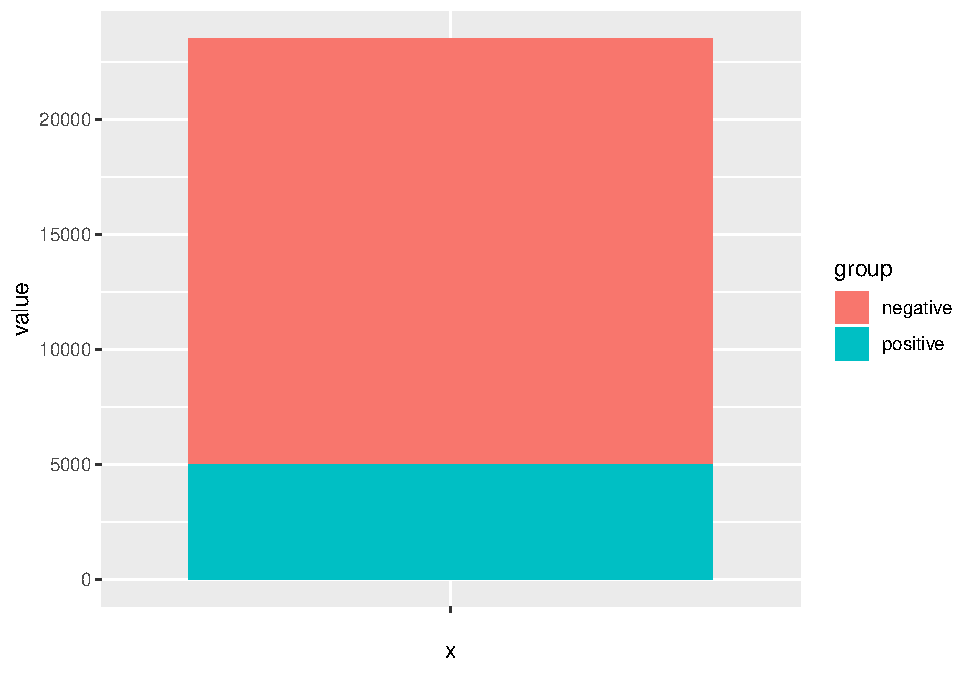
\includegraphics{jabstb_files/figure-latex/unnamed-chunk-51-1.pdf}

\hypertarget{side-by-side-bar-chart}{%
\paragraph{Side-by-side bar chart}\label{side-by-side-bar-chart}}

Note: There is no error to report. There's no variation. Cells were classified as either having or not having the antigen.

\begin{Shaded}
\begin{Highlighting}[]
\KeywordTok{ggplot}\NormalTok{(}
\NormalTok{  prop.df, }
\NormalTok{  (}\KeywordTok{aes}\NormalTok{(}
    \DataTypeTok{x=}\NormalTok{group, }
    \DataTypeTok{y=}\NormalTok{value, }
    \DataTypeTok{fill=}\NormalTok{group)}
\NormalTok{   )}
\NormalTok{  ) }\OperatorTok{+}
\StringTok{  }\KeywordTok{geom_bar}\NormalTok{(}\DataTypeTok{stat=}\StringTok{"identity"}\NormalTok{)}
\end{Highlighting}
\end{Shaded}

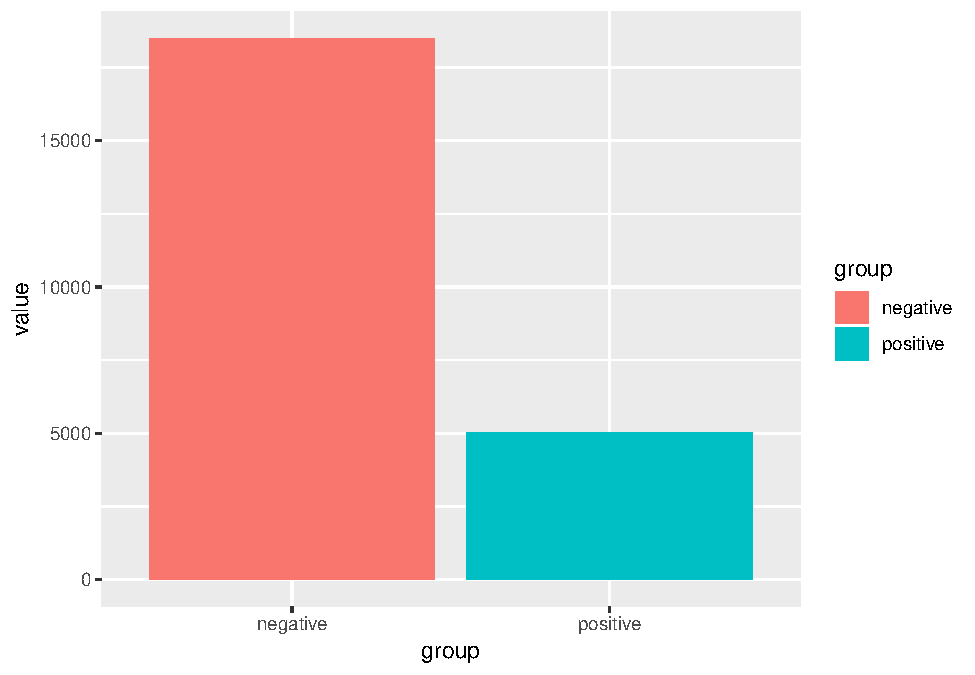
\includegraphics{jabstb_files/figure-latex/unnamed-chunk-52-1.pdf}

..

\bibliography{book.bib,packages.bib}


\end{document}
